% !TEX root = ../main.tex
%
\begin{appendices}

\chapter{Appendix}

This appendix is devoted to the illustration of the additional plot related to the study of the Partial
Event Mixing model described in Section~\ref{sec:pem}.

%
\section{PEM model additional plot} \label{app:pem}

In the following the full list of figures related to the data-model \ -- i.e. PEM model -- \ comparison, with 
the blinded RoI, is presented.
This study has been performed in the $0.0 - 4.0\ \gevc$ transverse momentum interval,
since for higher \pt the \ds production is expected to be negligible.

\begin{figure}[htb]
\begin{subfigure}{.5\textwidth}
  \centering
  \captionsetup{justification=centering}
  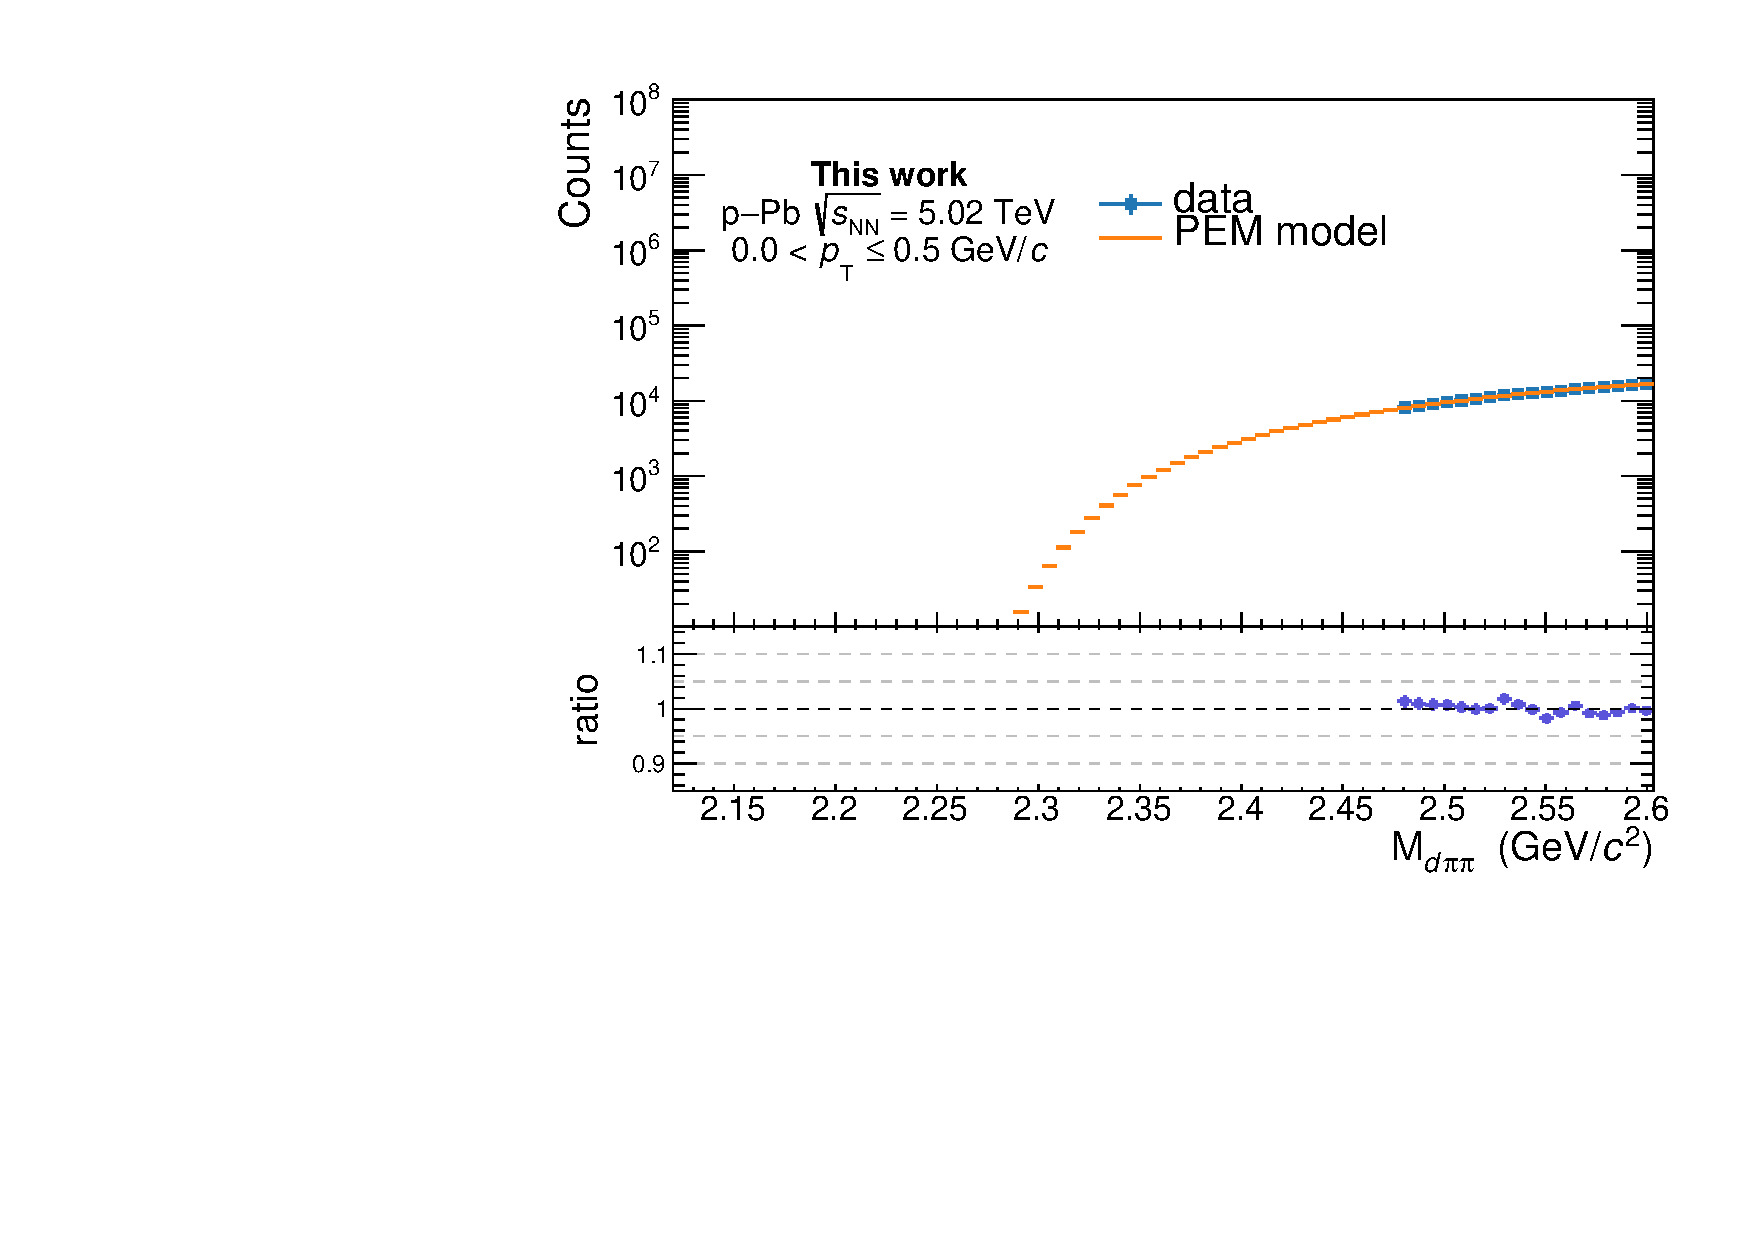
\includegraphics[width=\linewidth]{gfx/appendix/pem/can_blindPEM0}
  \caption{}
\end{subfigure}%
\begin{subfigure}{.5\textwidth}
  \centering
  \captionsetup{justification=centering}
  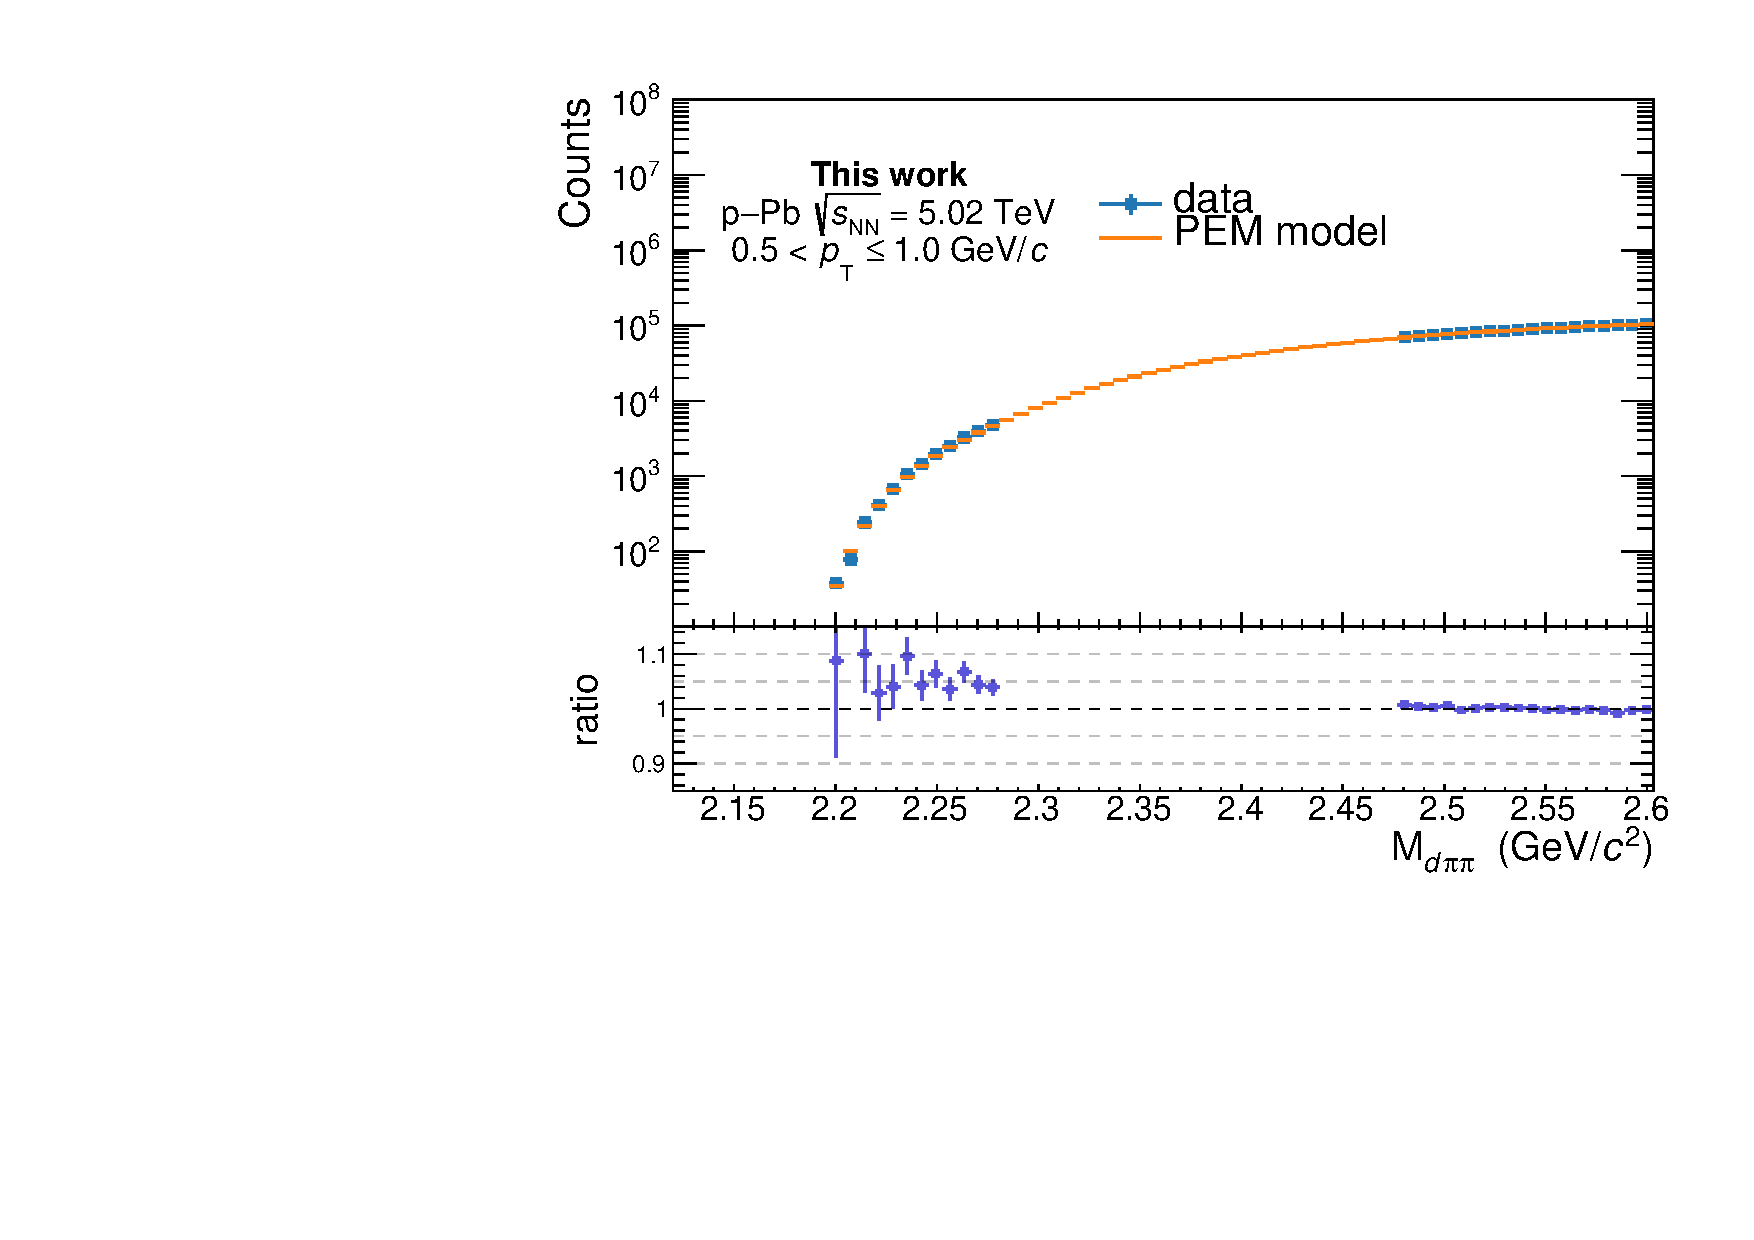
\includegraphics[width=\linewidth]{gfx/appendix/pem/can_blindPEM1}
  \caption{}
\end{subfigure}
\begin{subfigure}{.5\textwidth}
  \centering
  \captionsetup{justification=centering}
  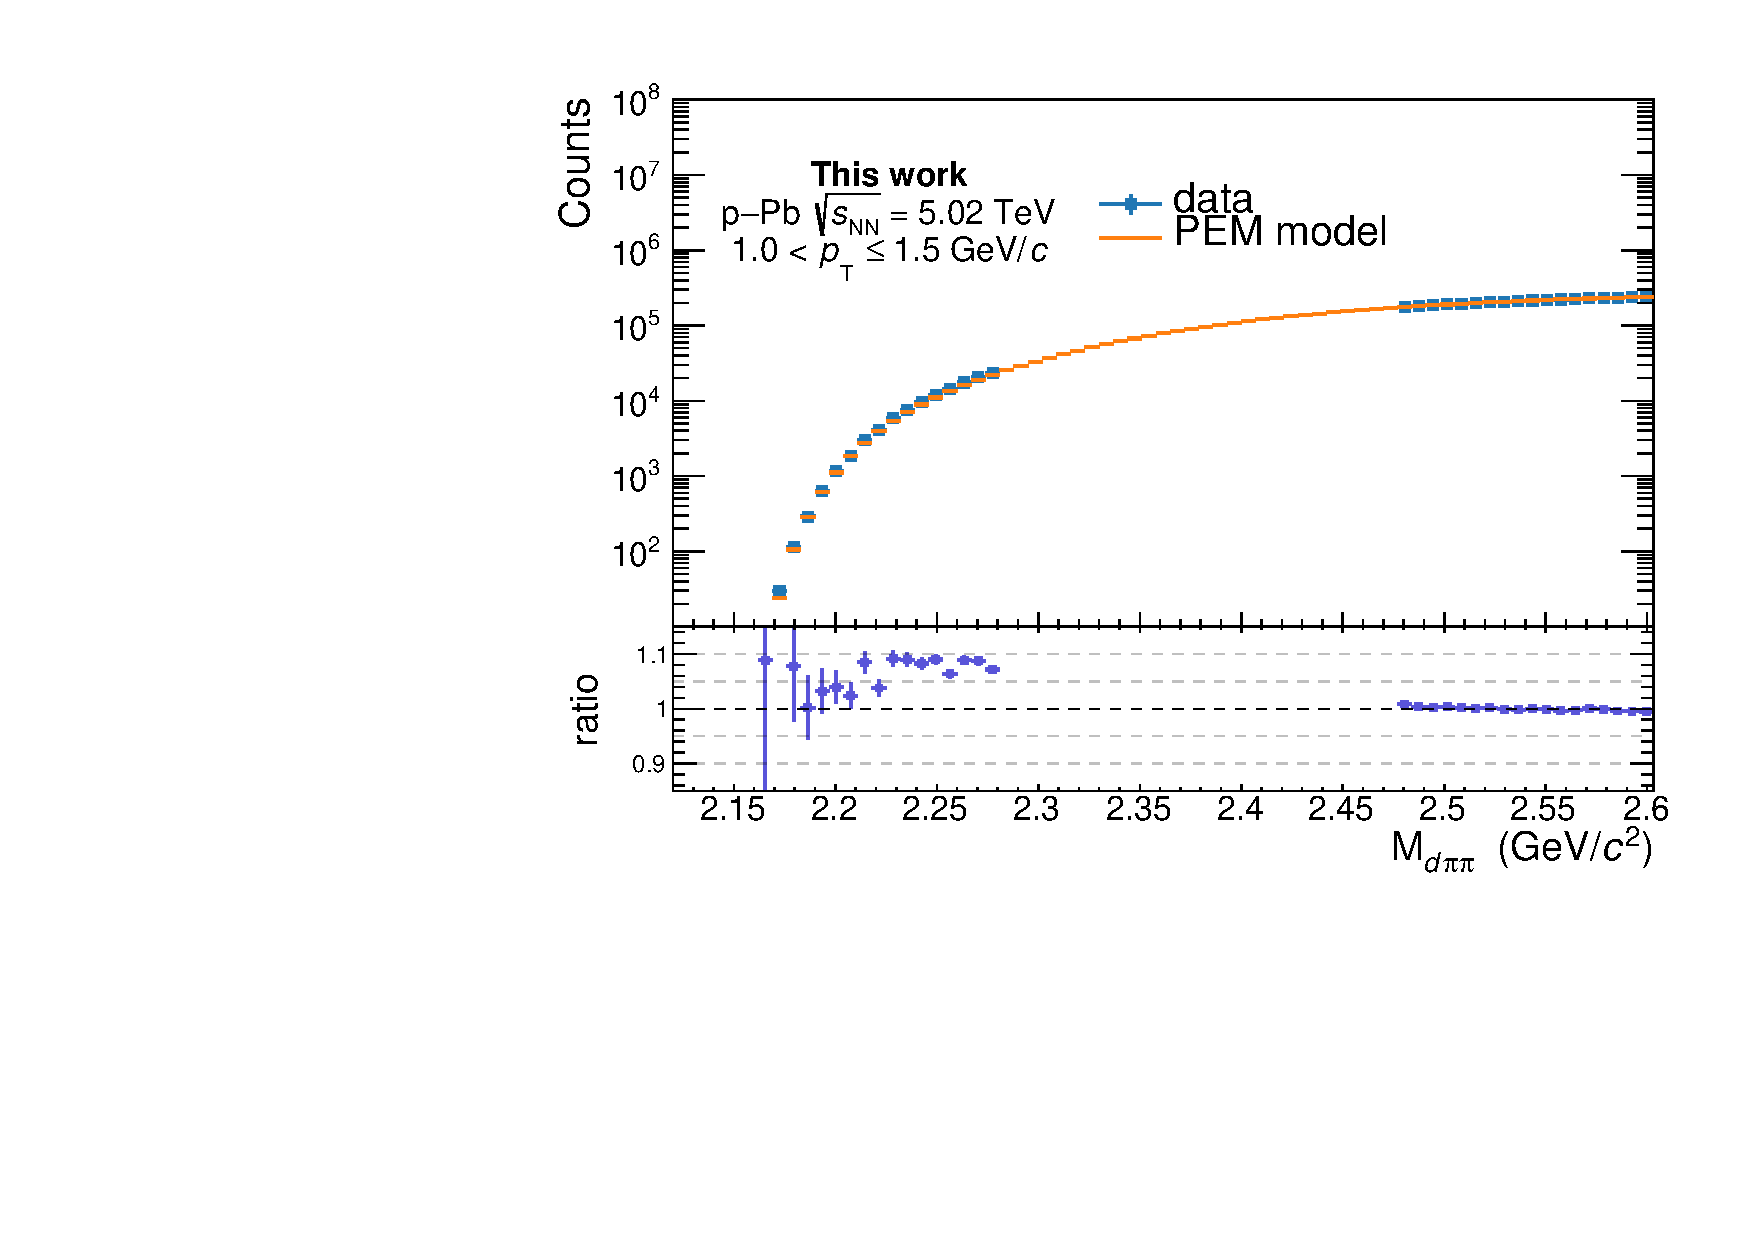
\includegraphics[width=\linewidth]{gfx/appendix/pem/can_blindPEM2}
  \caption{}
\end{subfigure}%
\begin{subfigure}{.5\textwidth}
  \centering
  \captionsetup{justification=centering}
  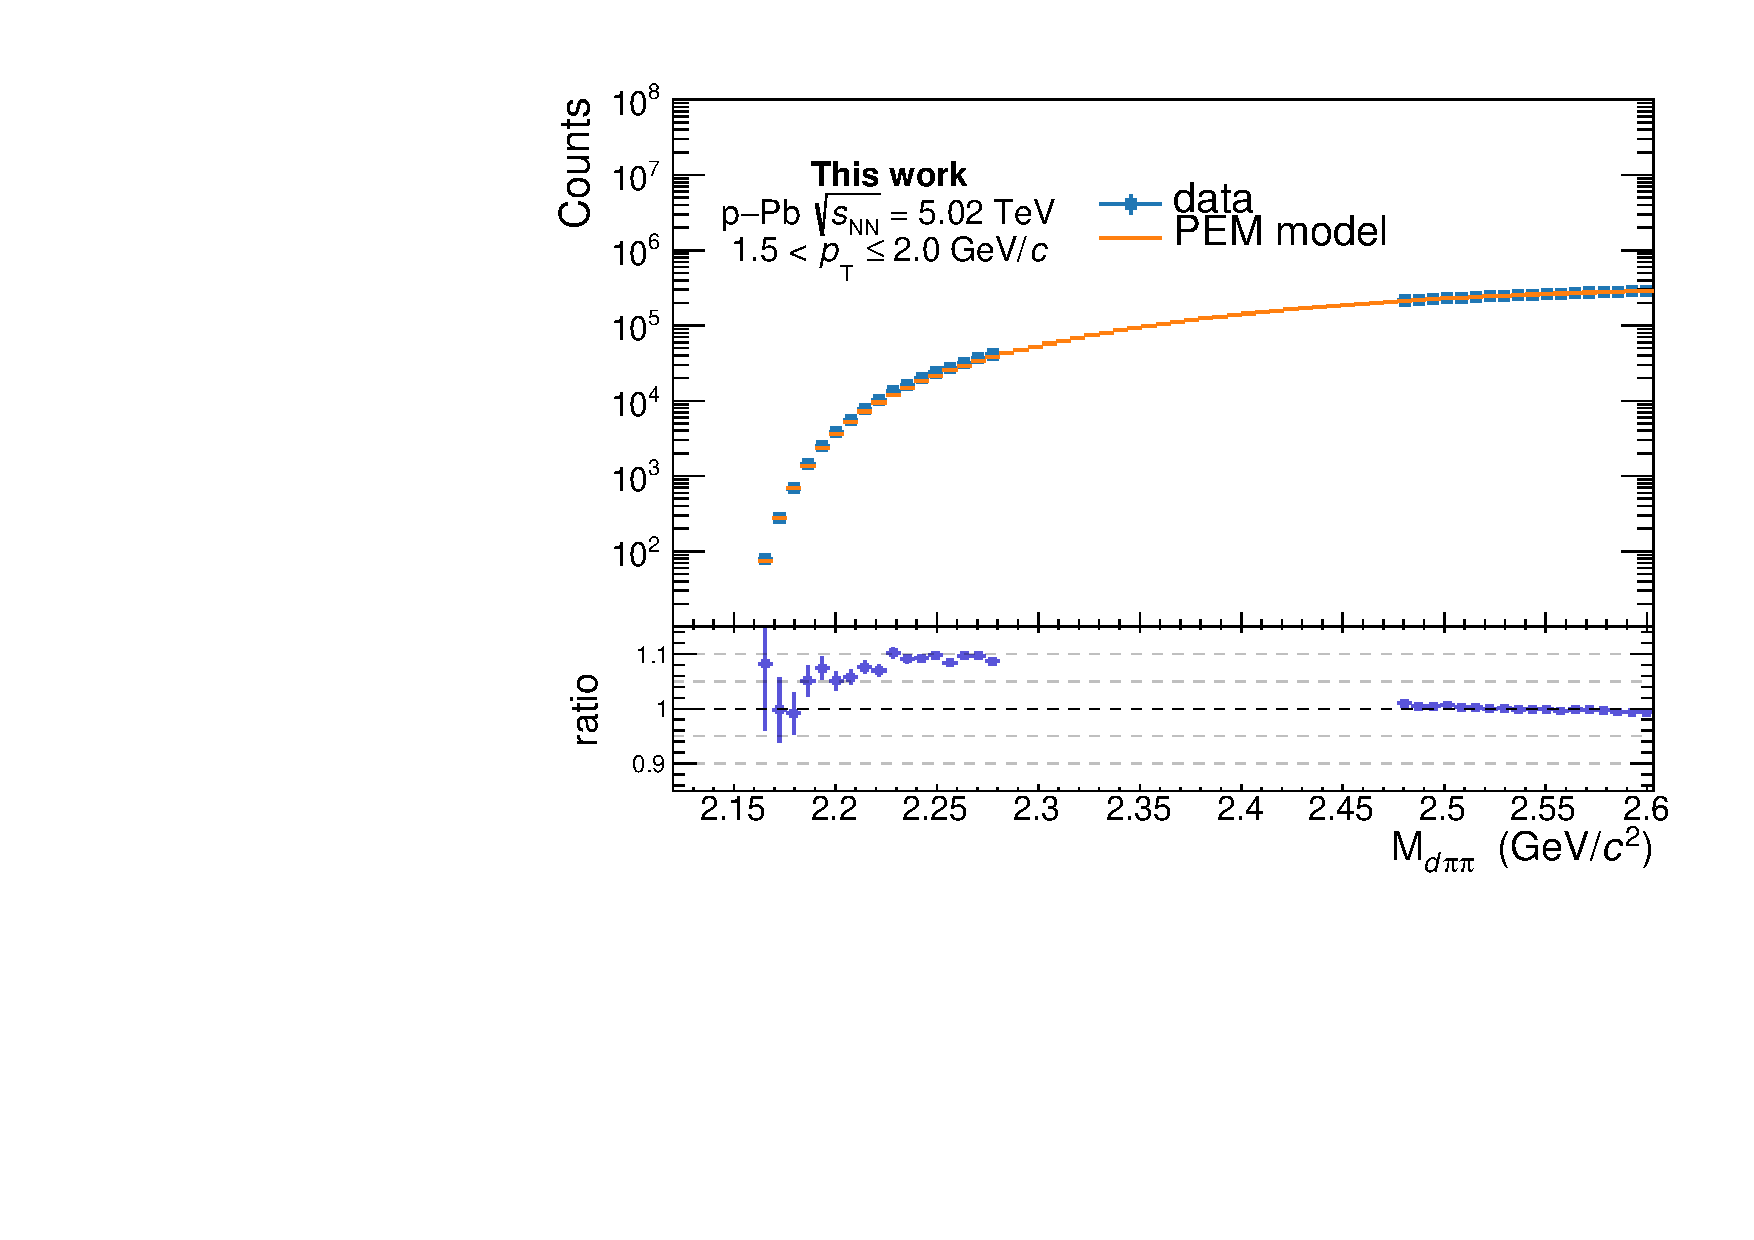
\includegraphics[width=\linewidth]{gfx/appendix/pem/can_blindPEM3}
  \caption{}
\end{subfigure}
\caption{PEM model compared with \minv, outside the region of interest. In the lower pad the data/model ratio is reported. Panel (a) shows the data-model comparison in the $0.0 < \pt \leq 0.5 \ \gevc$ interval, while Panels (b), (c) and (d) in the $0.5 < \pt \leq 1.0 \ \gevc$, $1.0 < \pt \leq 1.5 \ \gevc$ and $1.5 < \pt \leq 2.0 \ \gevc$ intervals respectively.}
\end{figure}

\begin{figure}[htb]
\begin{subfigure}{.5\textwidth}
  \centering
  \captionsetup{justification=centering}
  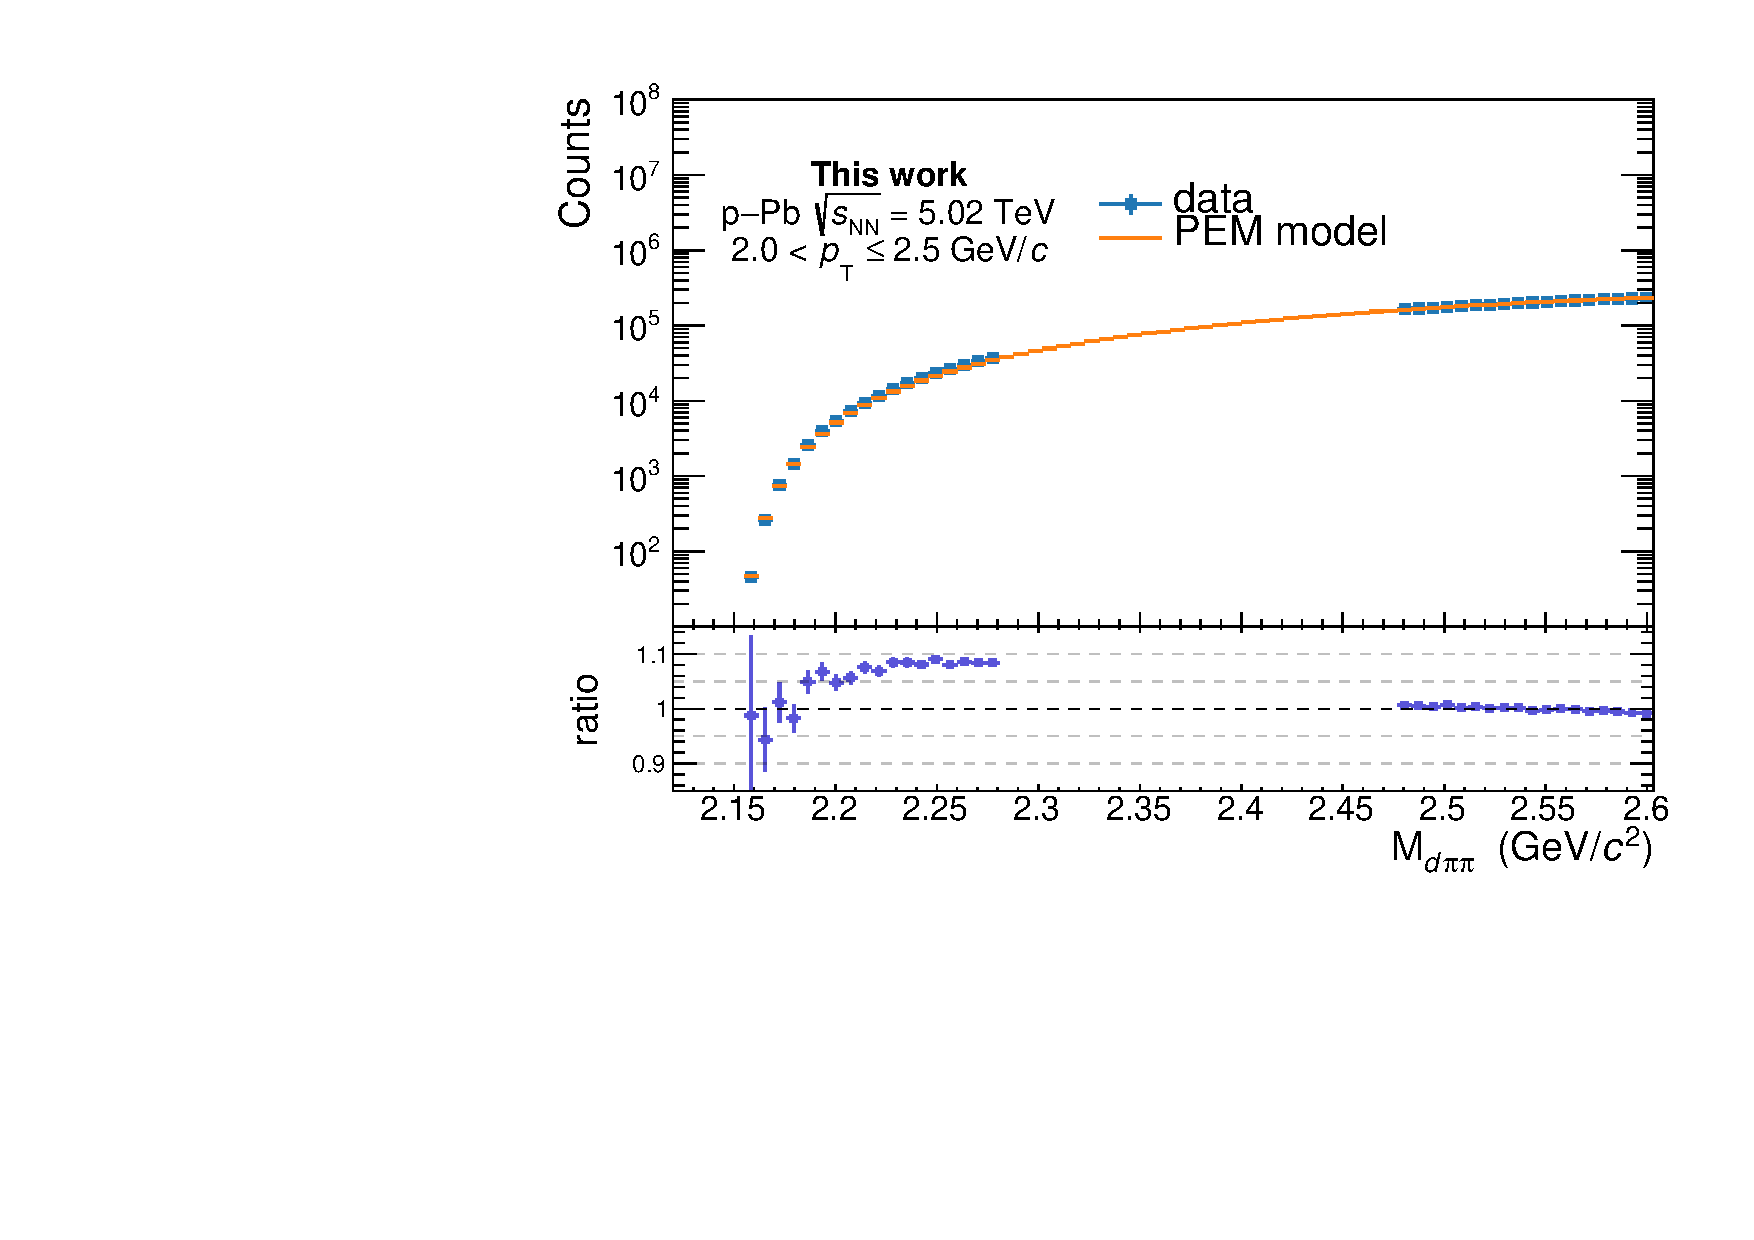
\includegraphics[width=\linewidth]{gfx/appendix/pem/can_blindPEM4}
  \caption{}
\end{subfigure}%
\begin{subfigure}{.5\textwidth}
  \centering
  \captionsetup{justification=centering}
  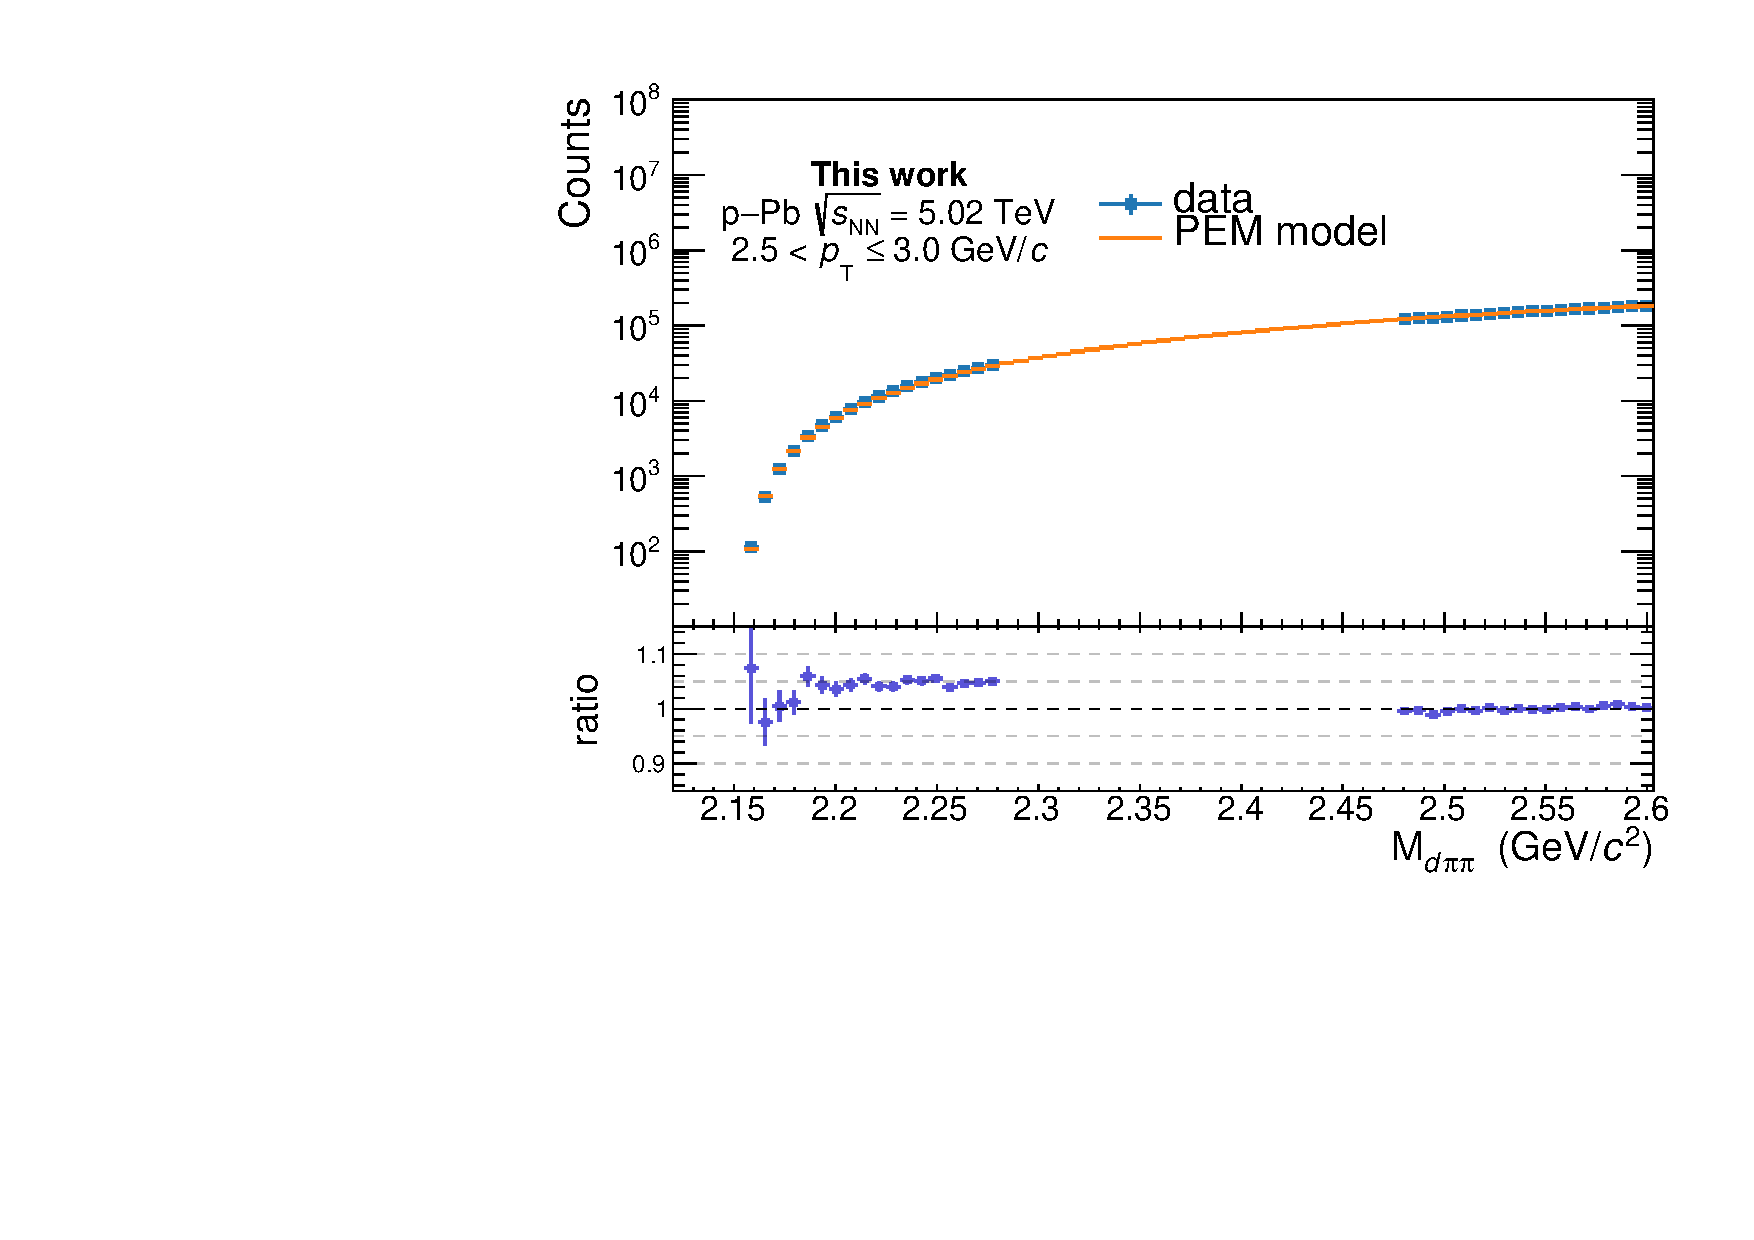
\includegraphics[width=\linewidth]{gfx/appendix/pem/can_blindPEM5}
  \caption{}
\end{subfigure}
\begin{subfigure}{.5\textwidth}
  \centering
  \captionsetup{justification=centering}
  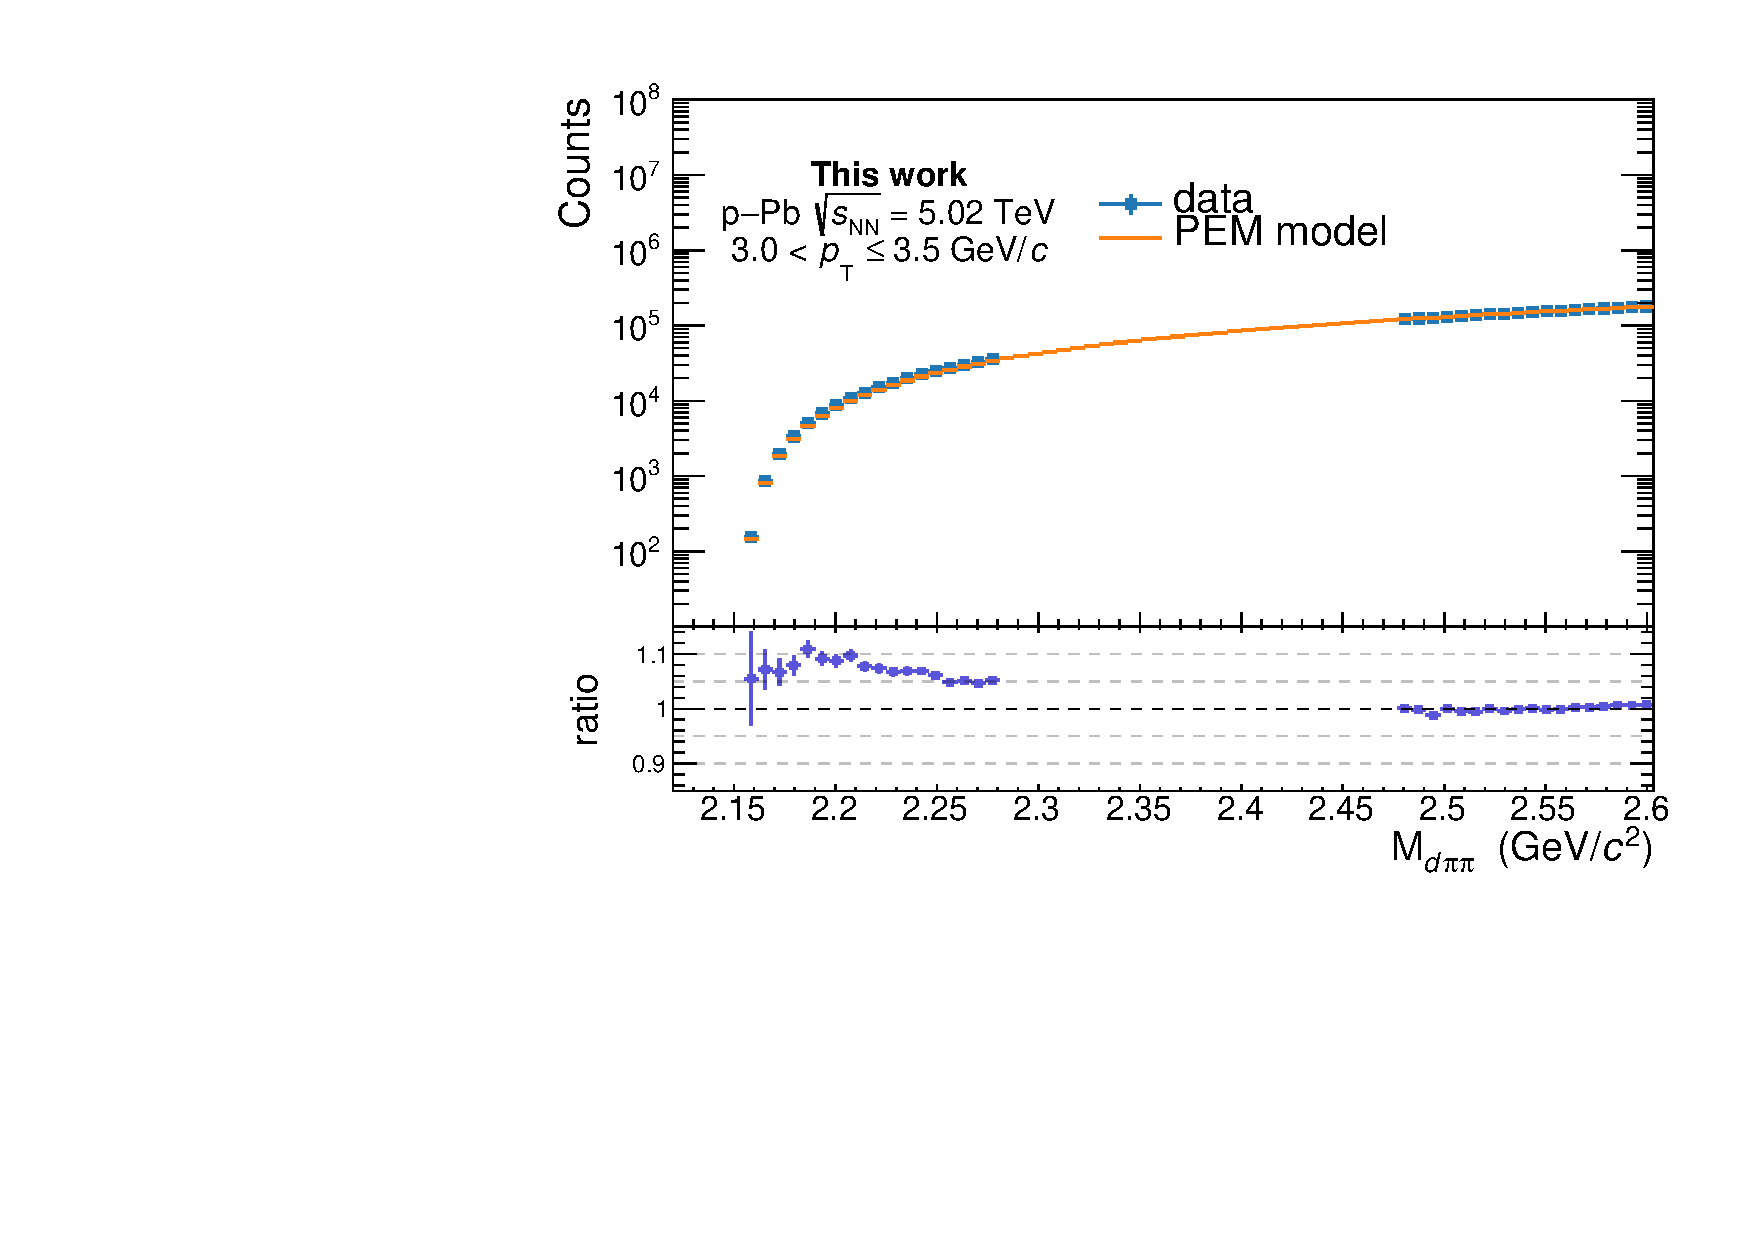
\includegraphics[width=\linewidth]{gfx/appendix/pem/can_blindPEM6}
  \caption{}
\end{subfigure}%
\begin{subfigure}{.5\textwidth}
  \centering
  \captionsetup{justification=centering}
  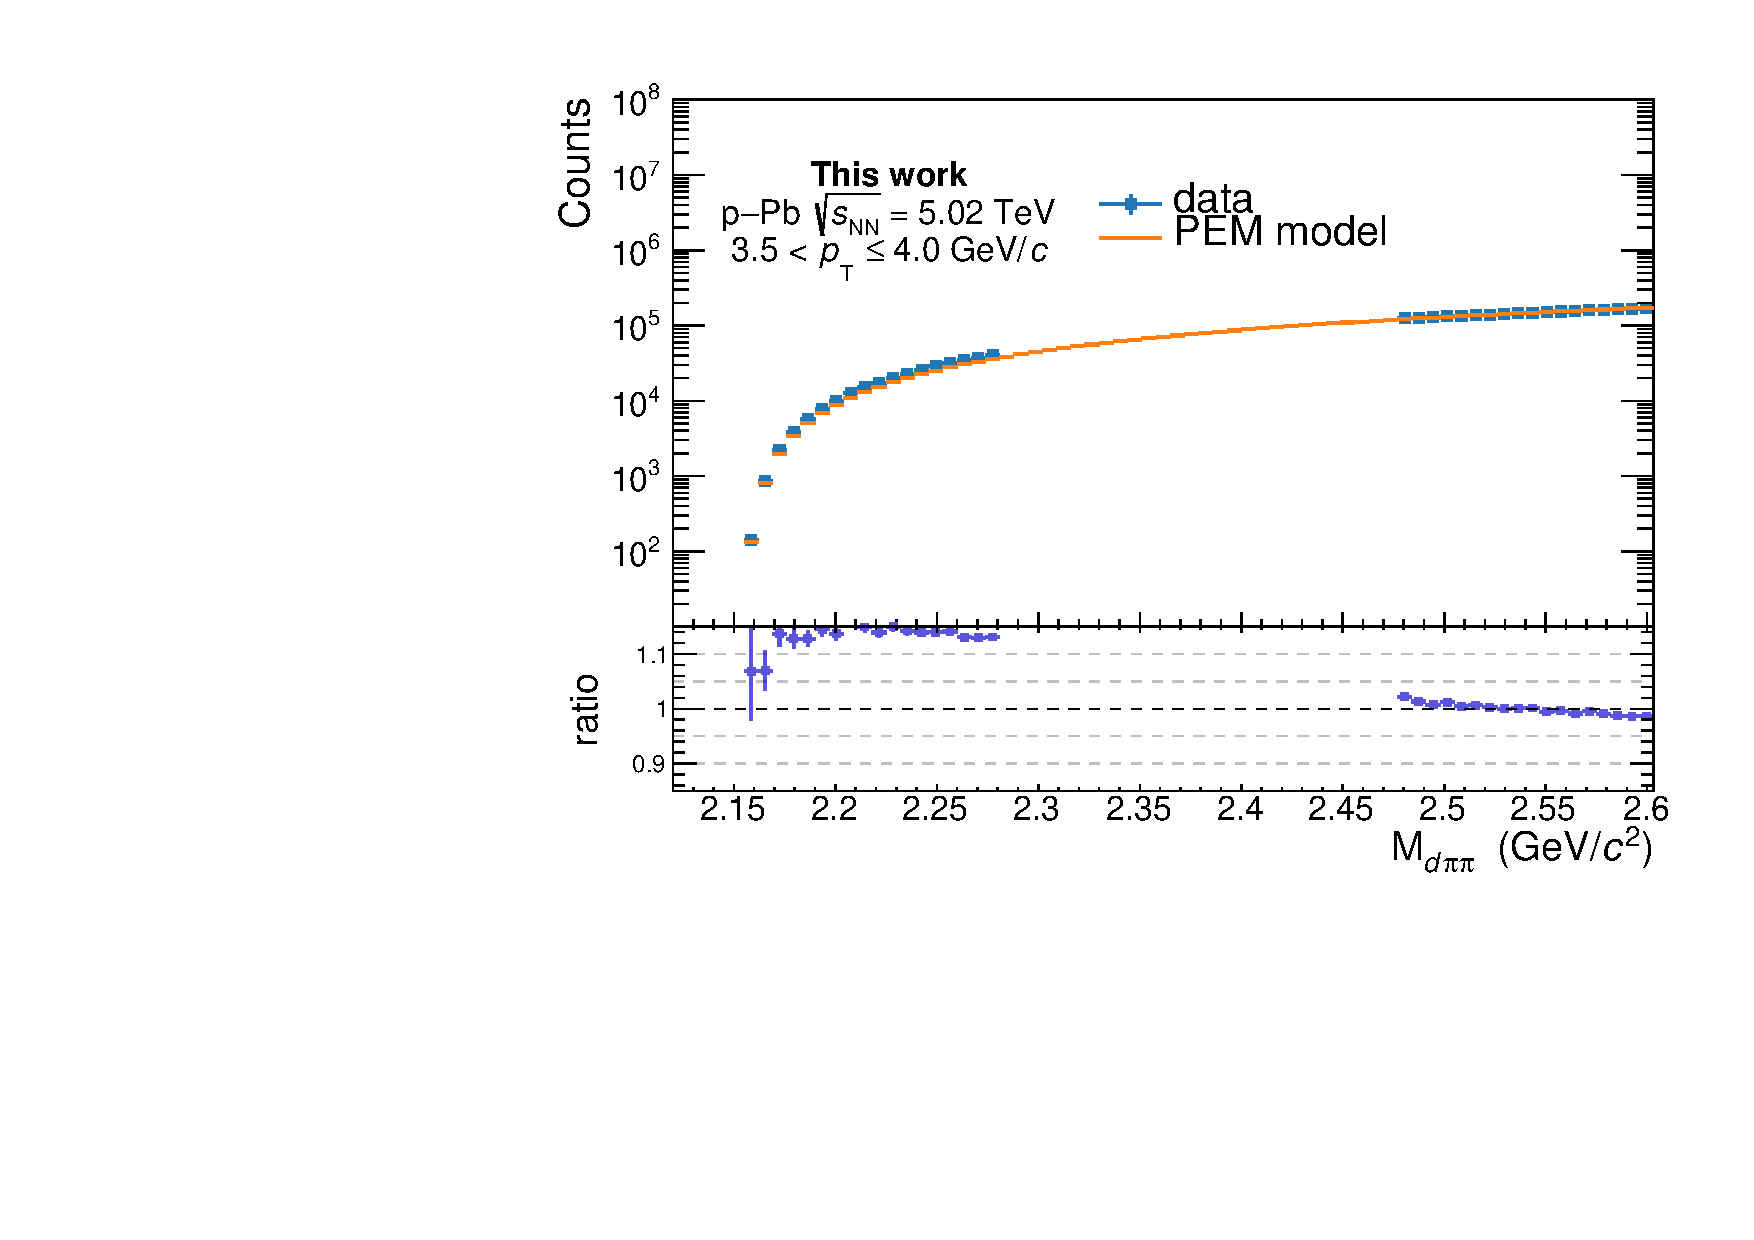
\includegraphics[width=\linewidth]{gfx/appendix/pem/can_blindPEM7}
  \caption{}
\end{subfigure}
\caption{PEM model compared with \minv, outside the region of interest. In the lower pad the data/model ratio is reported. Panel (a) shows the data-model comparison in the $2.0 < \pt \leq 2.5\ \gevc$ interval, while Panels (b), (c) and (d) in the $2.5 < \pt \leq 3.0\ \gevc$, $3.0 < \pt \leq 3.5\ \gevc$, $3.5 < \pt \leq 4.0\ \gevc$ intervals respectively.}
\end{figure}
\clearpage

%
%
\section{Improved PEM model additional plot} \label{app:pemimp}

In the following the full list of figures related to the data-model \ -- i.e. improved PEM model -- \
comparison, with the blinded RoI, is presented. 
This study has been performed in the $0.0 - 4.0\ \gevc$ transverse momentum interval,
since for higher \pt the \ds production is expected to be negligible.

\begin{figure}[!h]
\begin{subfigure}{.5\textwidth}
  \centering
  \captionsetup{justification=centering}
  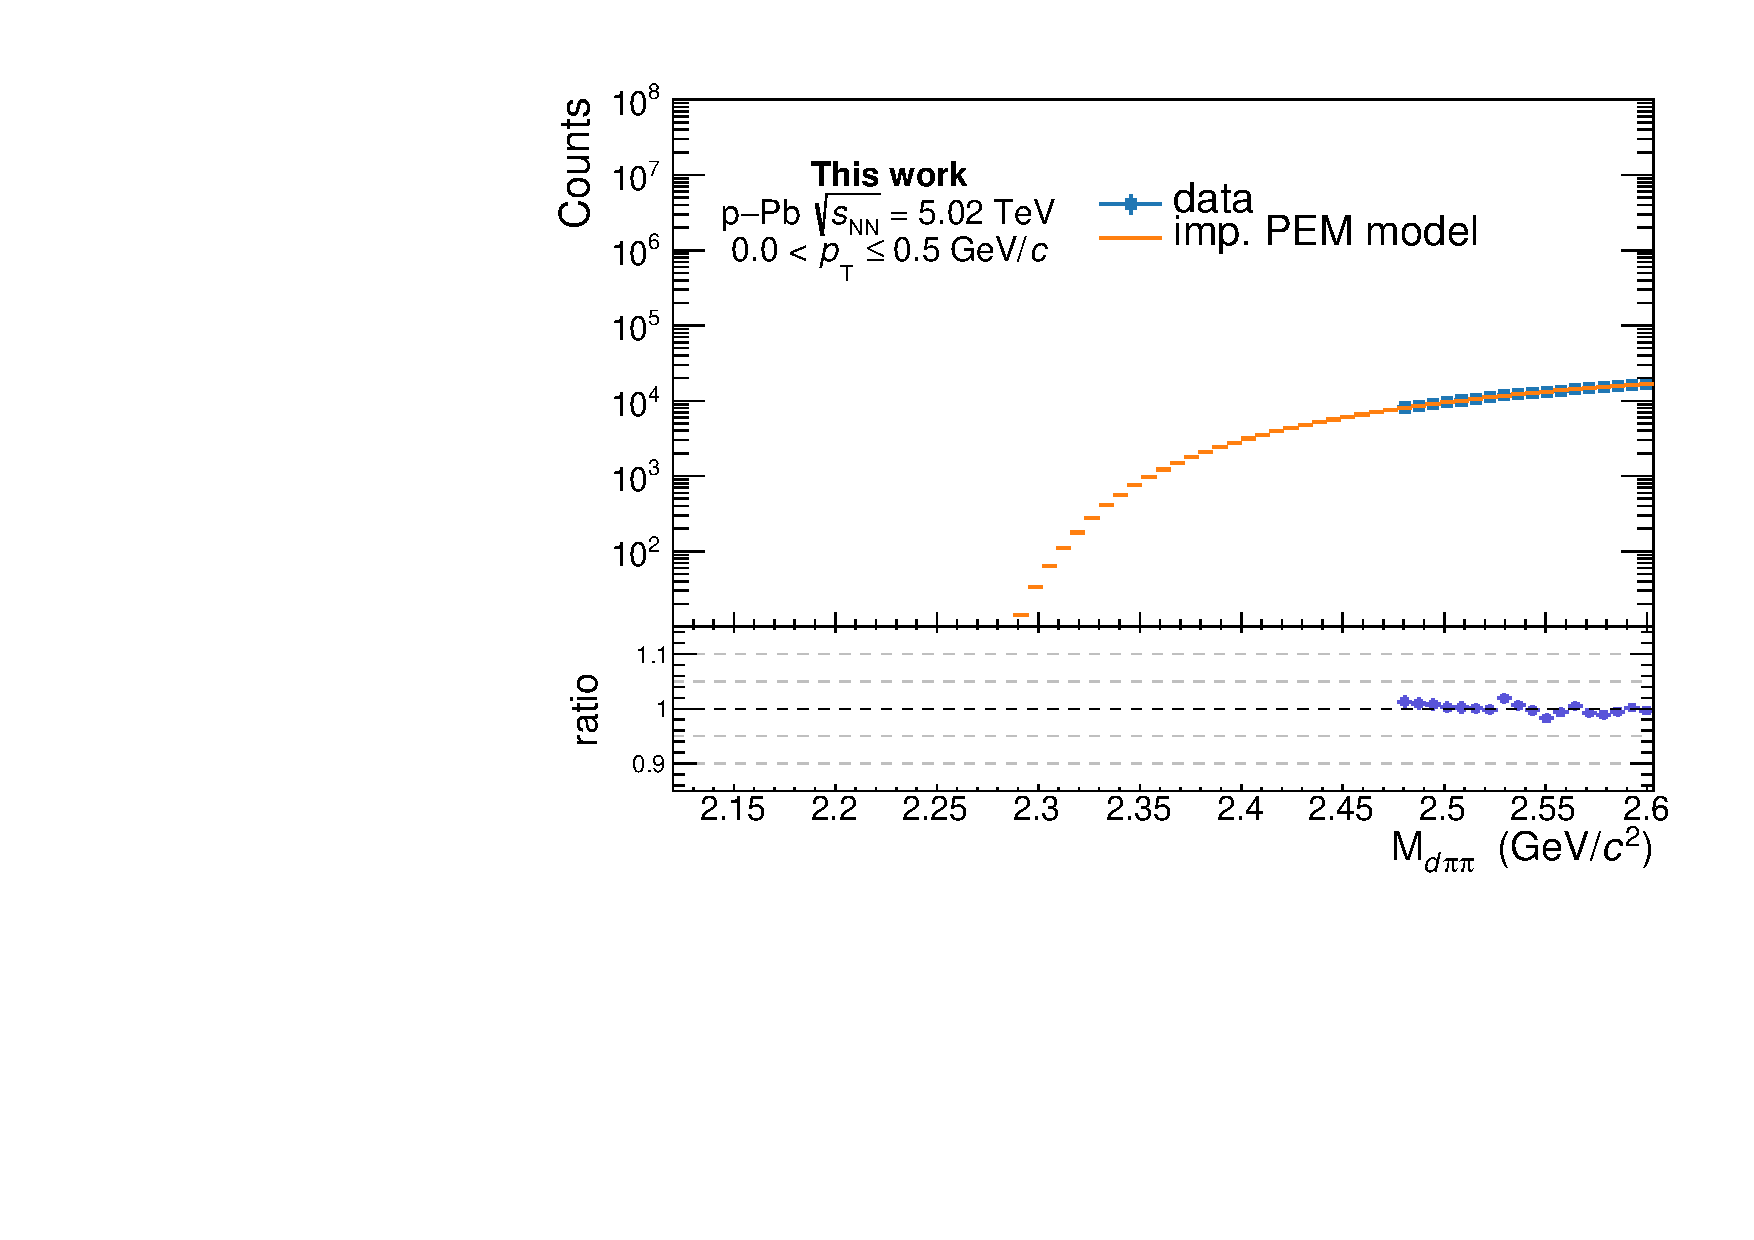
\includegraphics[width=\linewidth]{gfx/appendix/impem/can_blindPEMimp0}
  \caption{}
\end{subfigure}%
\begin{subfigure}{.5\textwidth}
  \centering
  \captionsetup{justification=centering}
  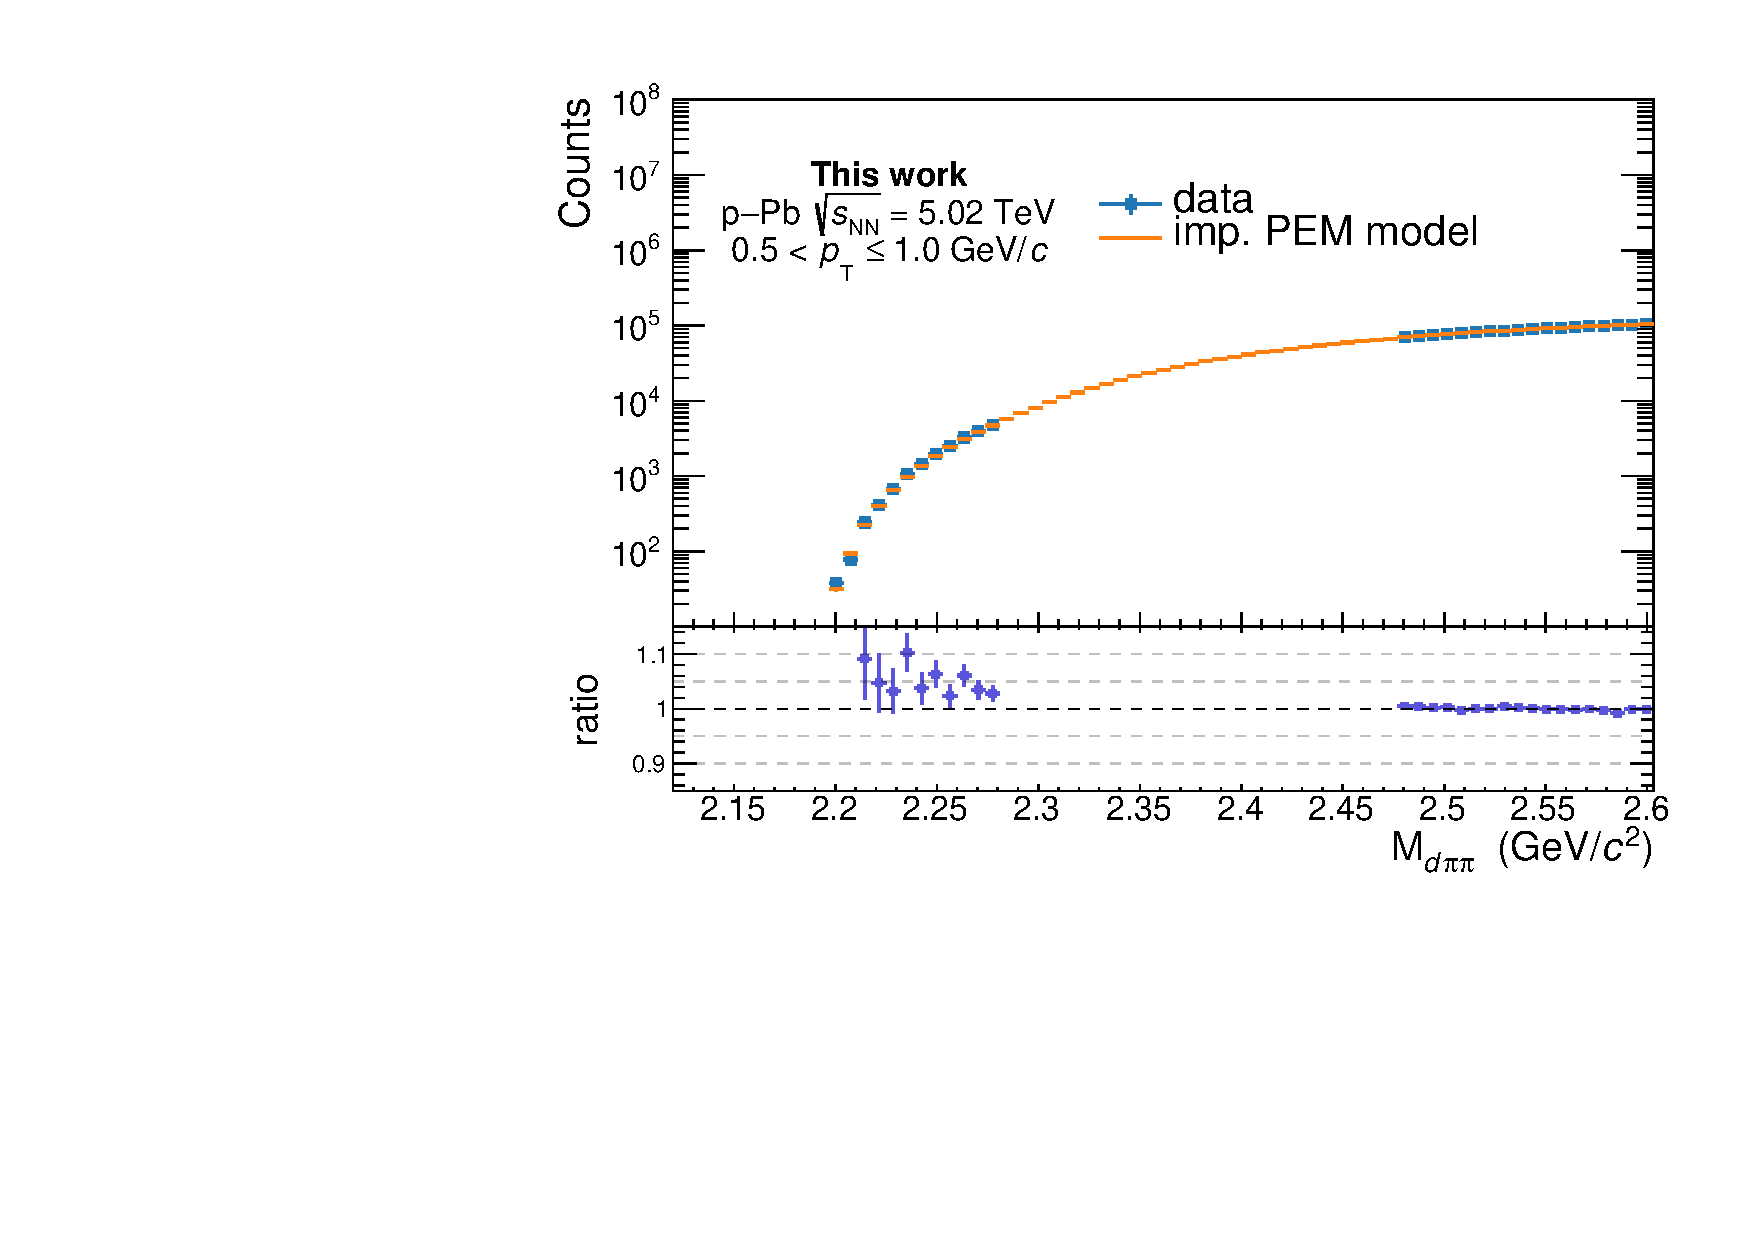
\includegraphics[width=\linewidth]{gfx/appendix/impem/can_blindPEMimp1}
  \caption{}
\end{subfigure}
\begin{subfigure}{.5\textwidth}
  \centering
  \captionsetup{justification=centering}
  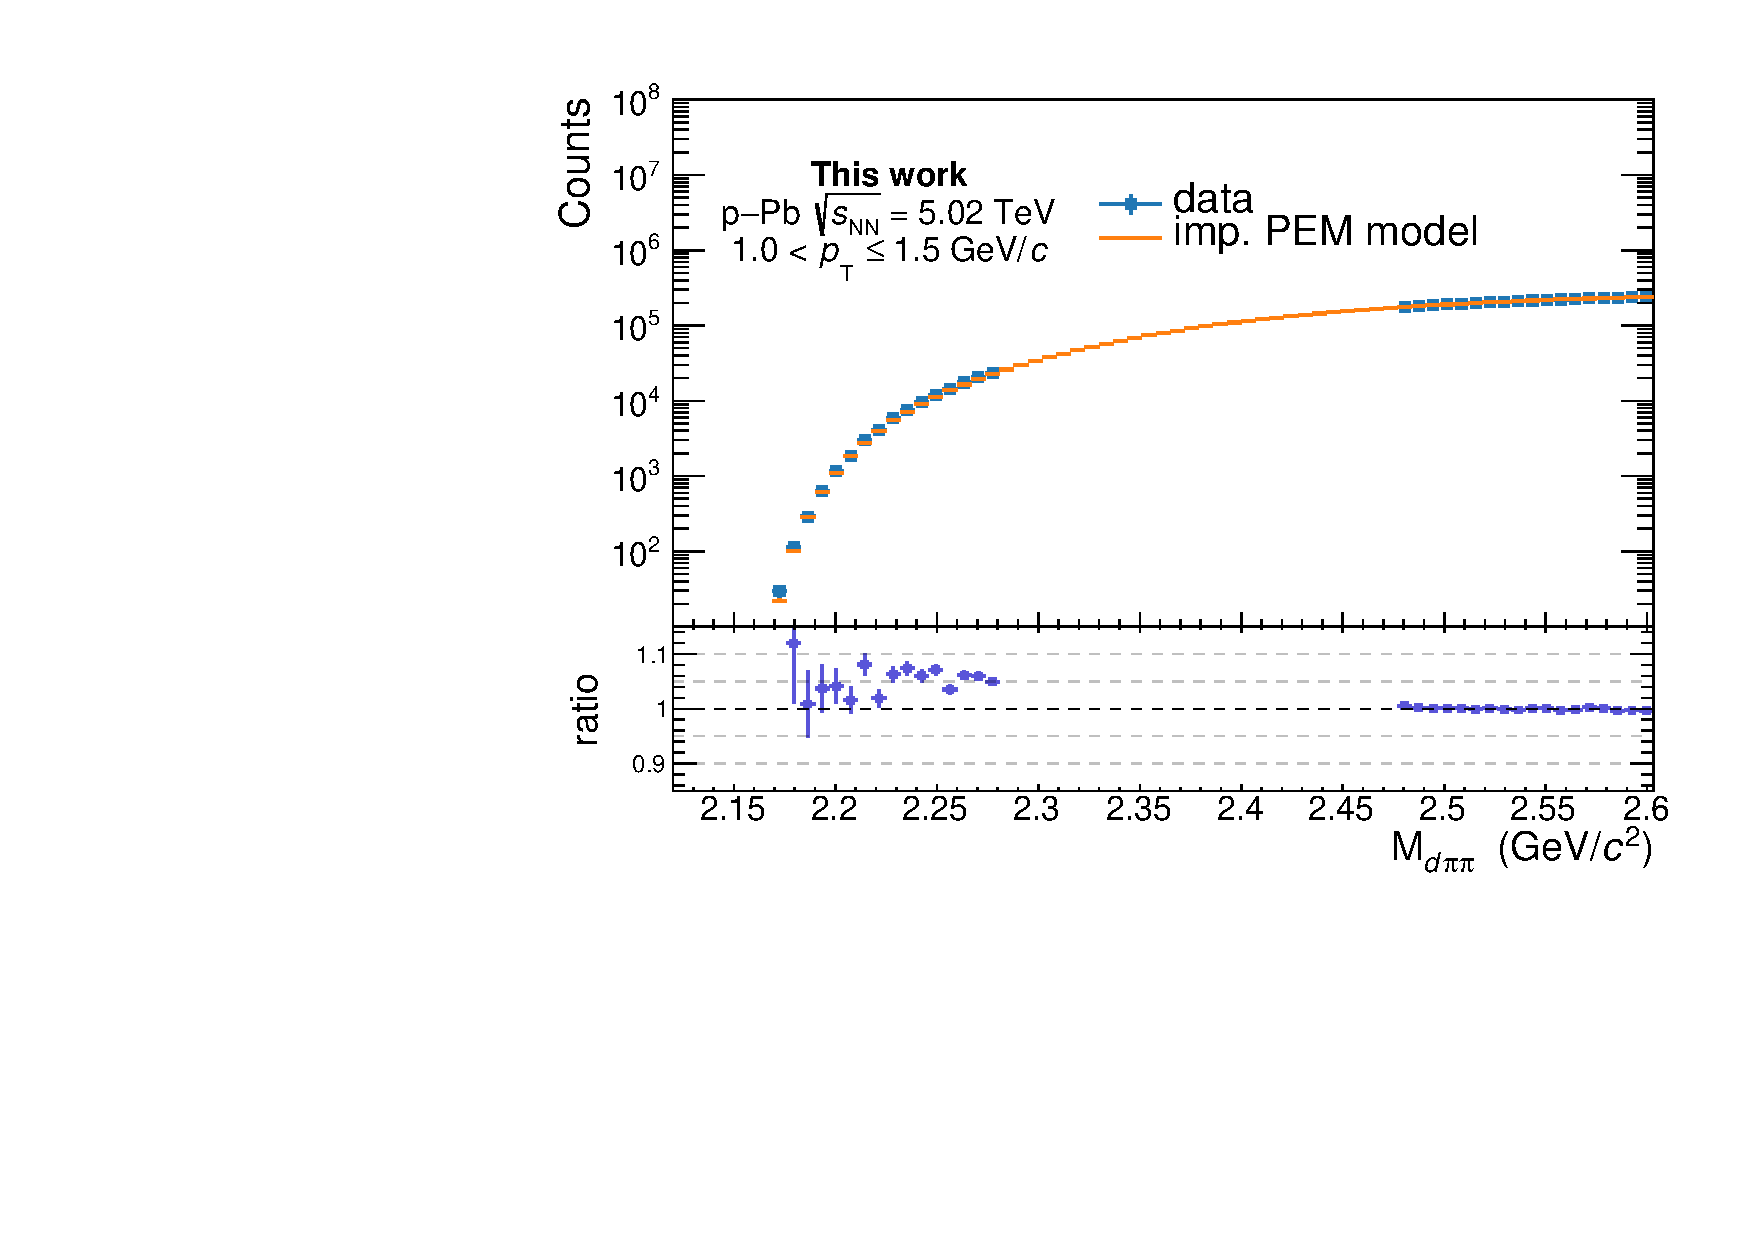
\includegraphics[width=\linewidth]{gfx/appendix/impem/can_blindPEMimp2}
  \caption{}
\end{subfigure}%
\begin{subfigure}{.5\textwidth}
  \centering
  \captionsetup{justification=centering}
  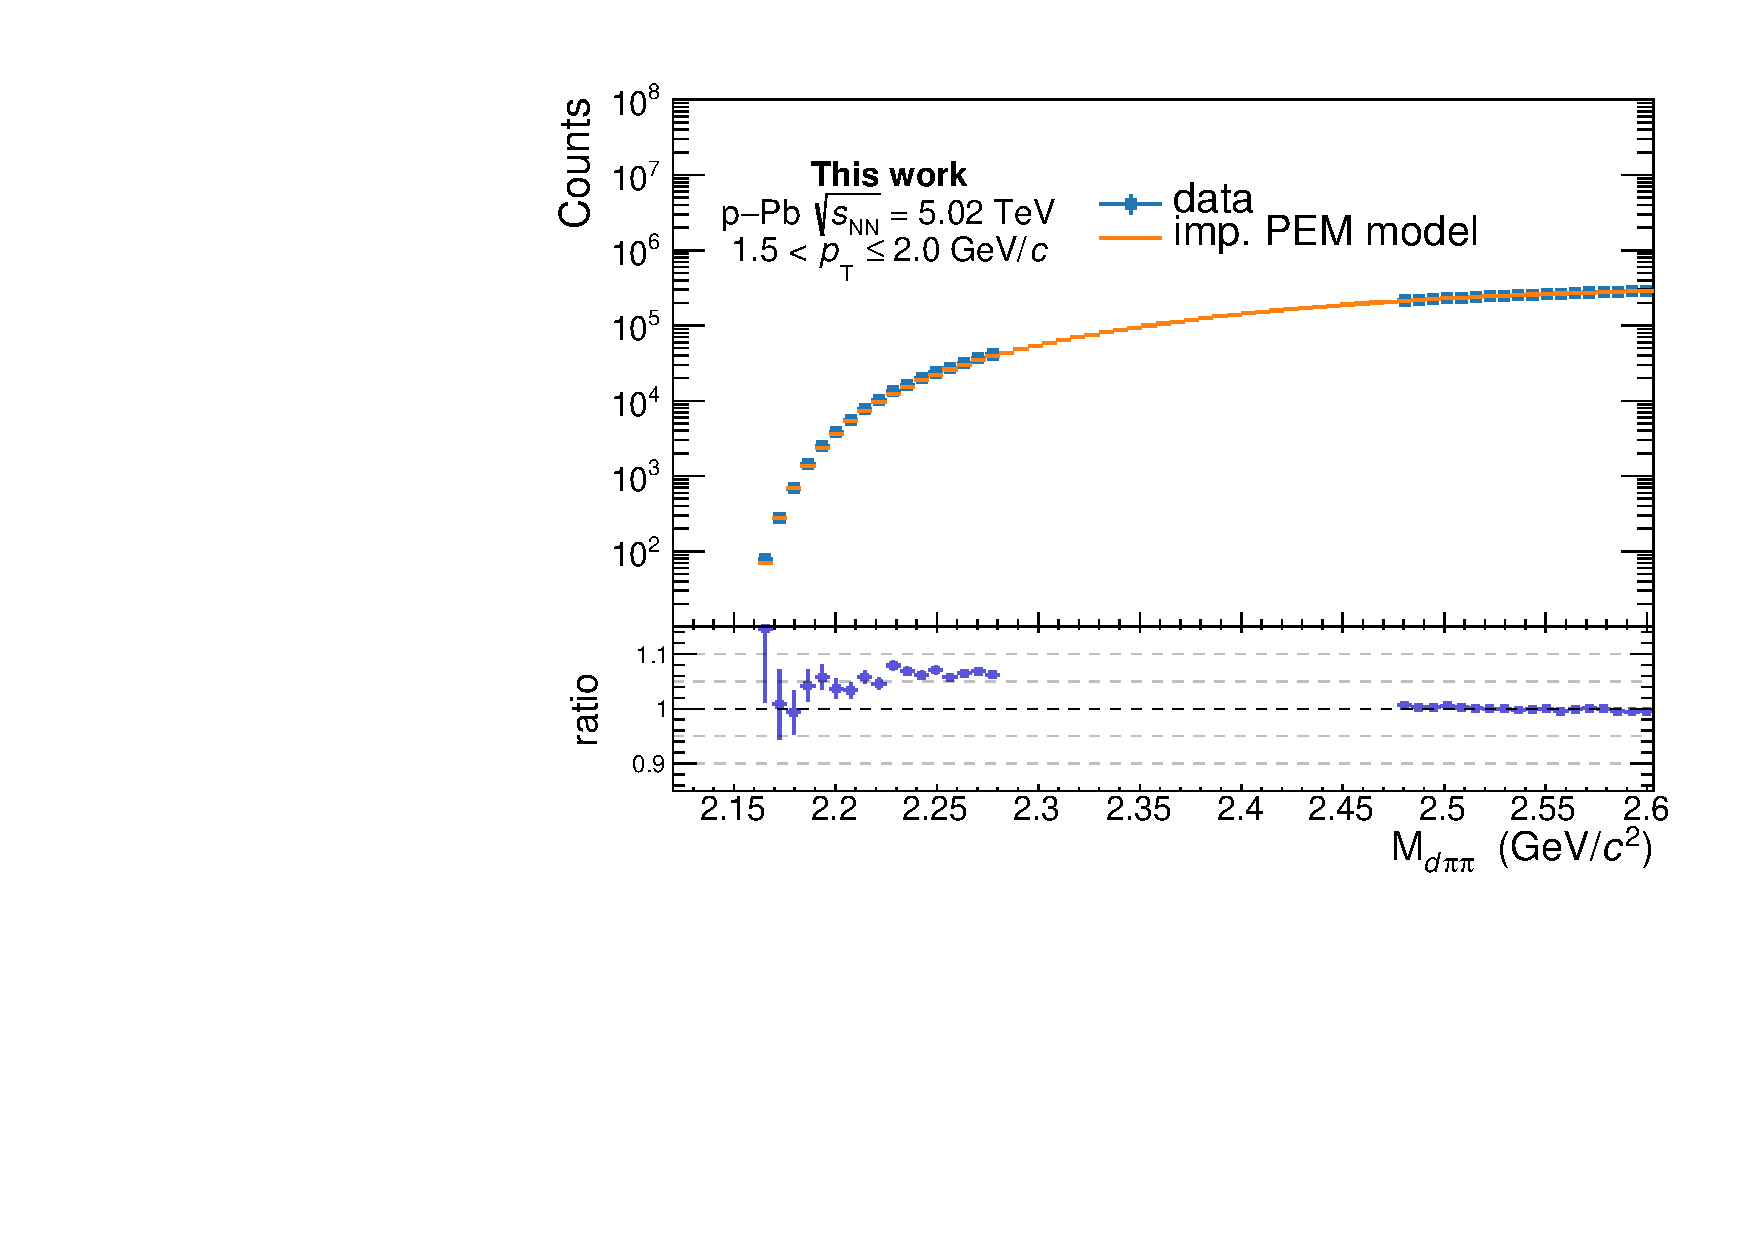
\includegraphics[width=\linewidth]{gfx/appendix/impem/can_blindPEMimp3}
  \caption{}
\end{subfigure}
\begin{subfigure}{.5\textwidth}
  \centering
  \captionsetup{justification=centering}
  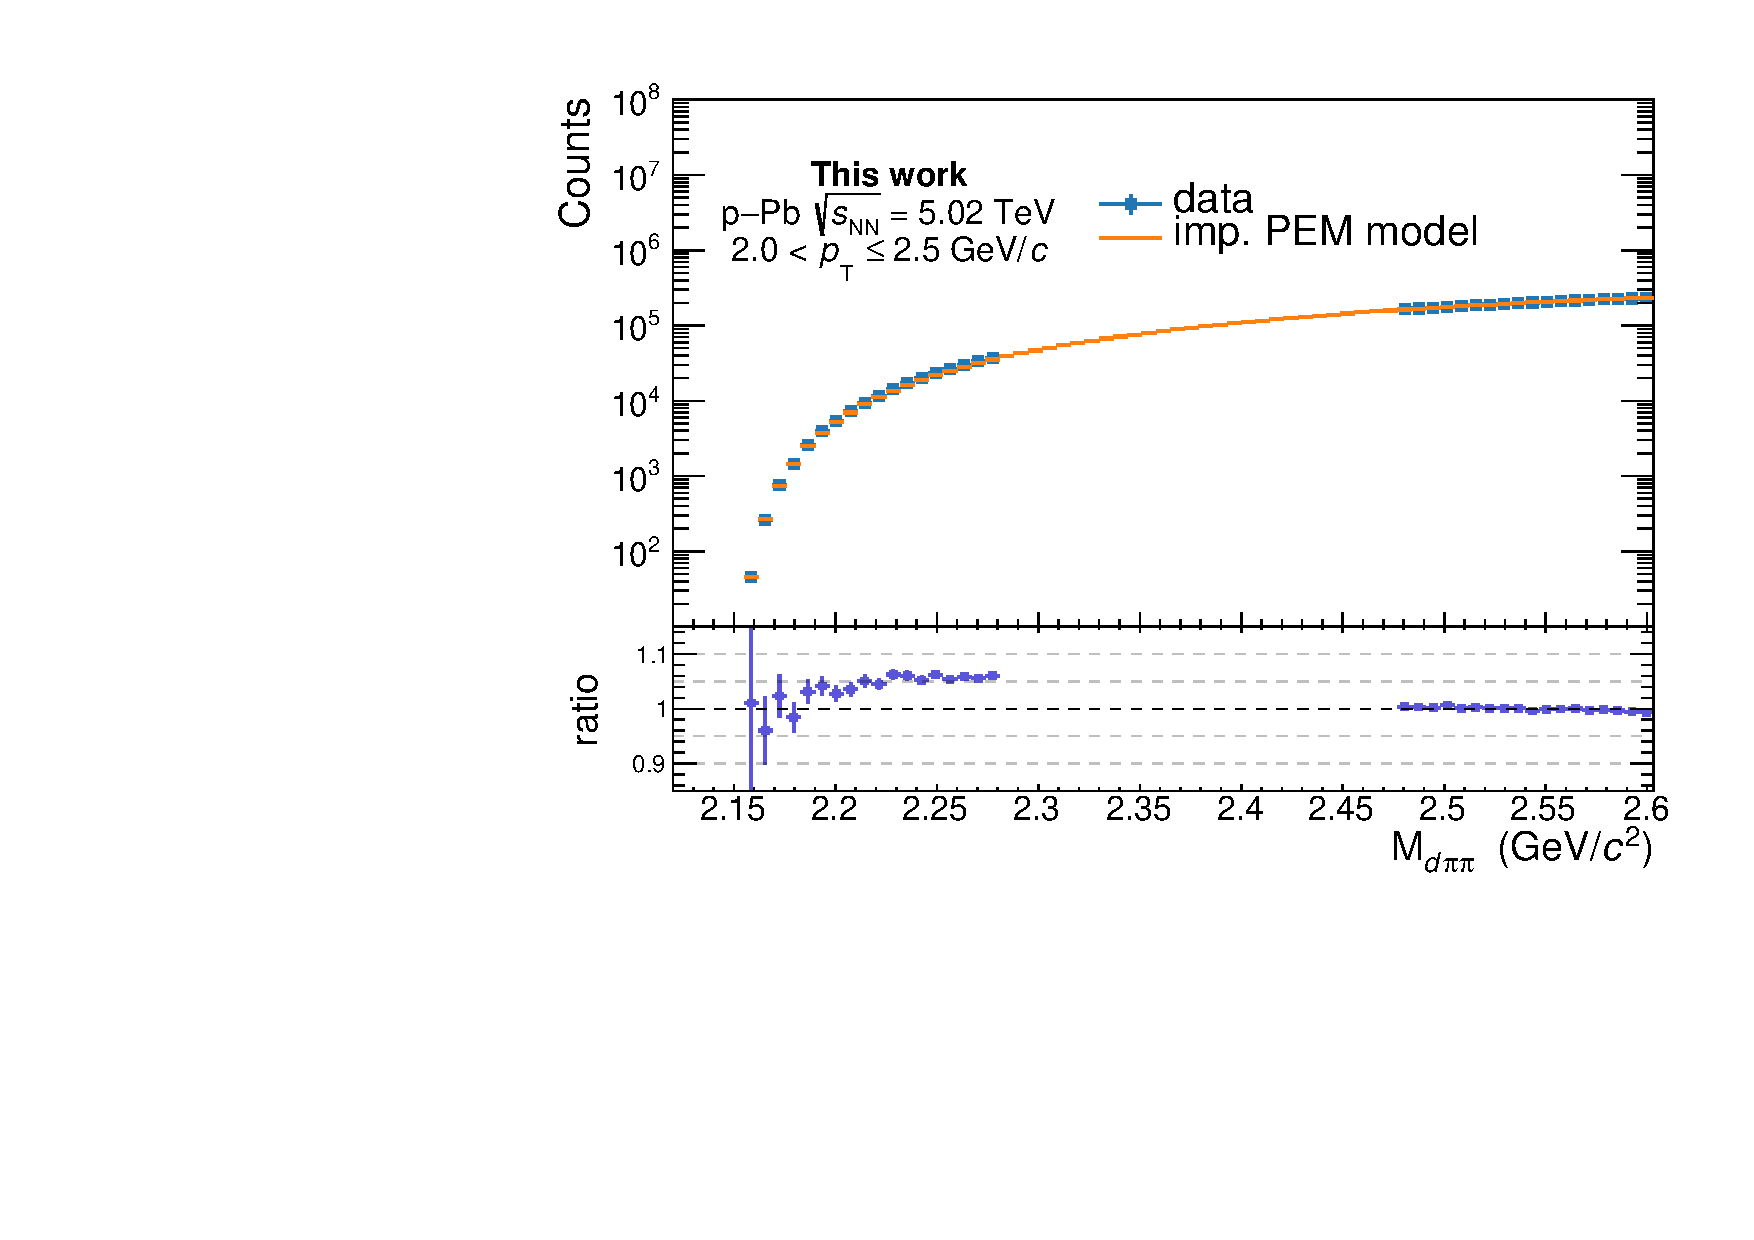
\includegraphics[width=\linewidth]{gfx/appendix/impem/can_blindPEMimp4}
  \caption{}
\end{subfigure}%
\begin{subfigure}{.5\textwidth}
  \centering
  \captionsetup{justification=centering}
  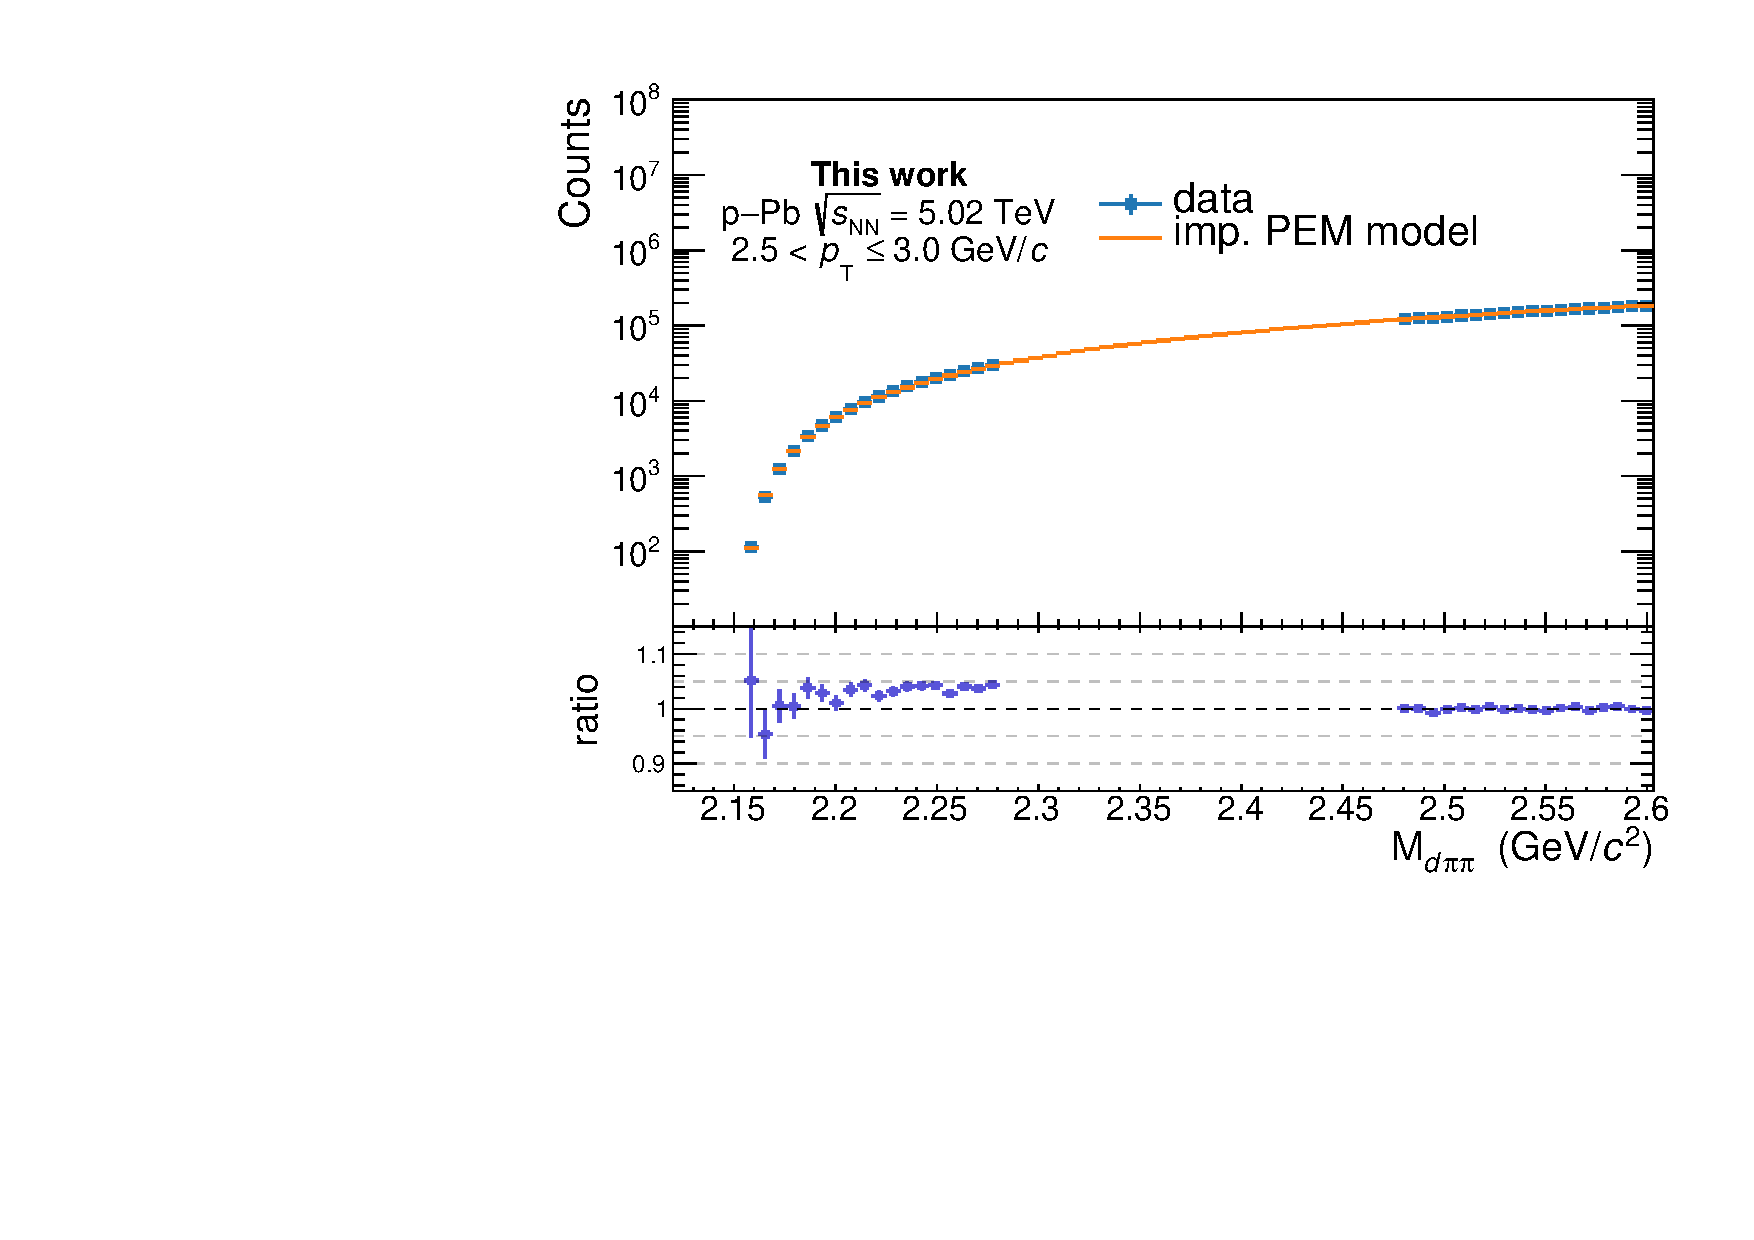
\includegraphics[width=\linewidth]{gfx/appendix/impem/can_blindPEMimp5}
  \caption{}
\end{subfigure}
\caption{Improved PEM model compared with \minv, outside the region of interest. In the lower pad the data/model ratio is reported. Panel (a) shows the data-model comparison in the $0.0 < \pt \leq 0.5\ \gevc$ interval, while Panels (b), (c), (d), (e) and (f), in the $0.5 < \pt \leq 1.0\ \gevc$, $1.0 < \pt \leq 1.5\ \gevc$, $1.5 < \pt \leq 2.0\ \gevc$, $2.0 < \pt \leq 2.5\ \gevc$ and $2.5 < \pt \leq 3.0\ \gevc$ intervals respectively.}
\end{figure}

\begin{figure}[!ht]
\begin{subfigure}{.5\textwidth}
  \centering
  \captionsetup{justification=centering}
  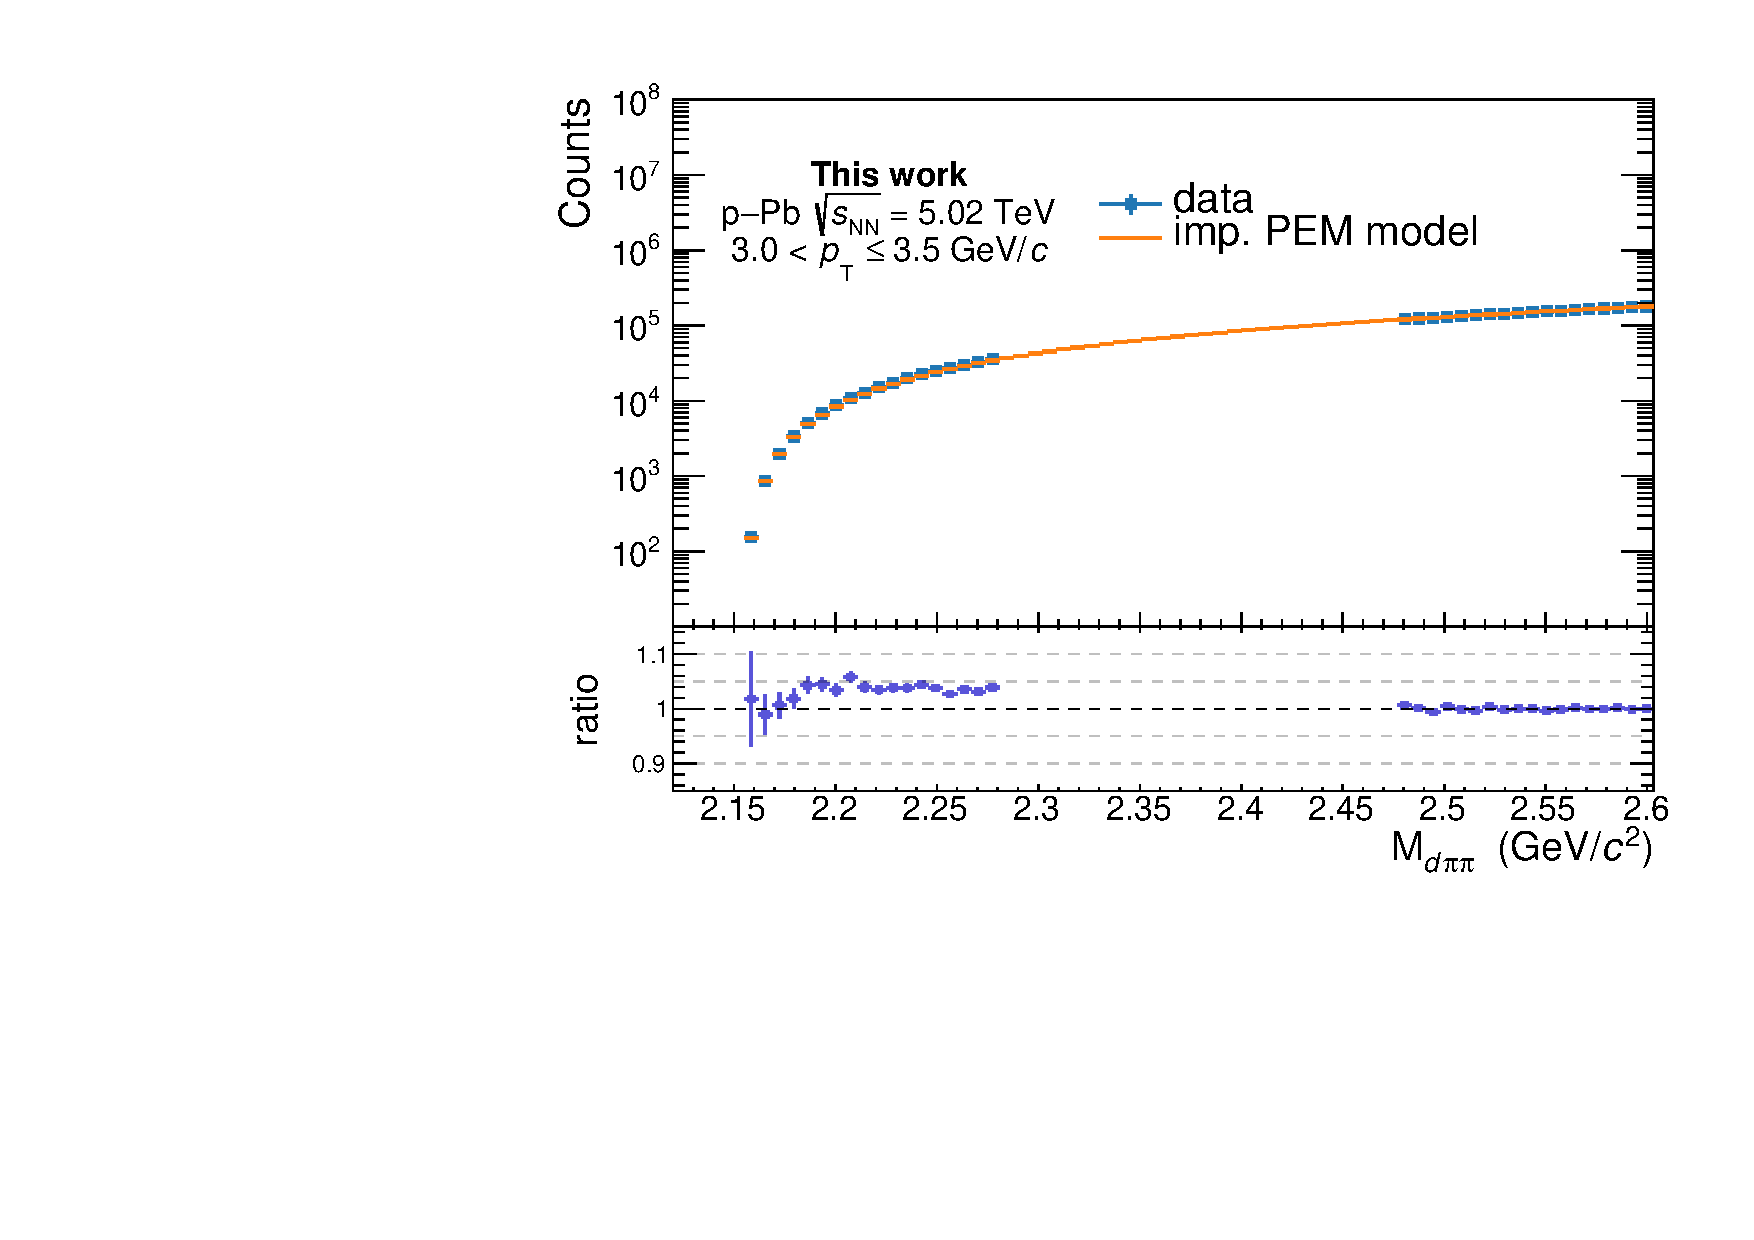
\includegraphics[width=\linewidth]{gfx/appendix/impem/can_blindPEMimp6}
  \caption{}
\end{subfigure}%
\begin{subfigure}{.5\textwidth}
  \centering
  \captionsetup{justification=centering}
  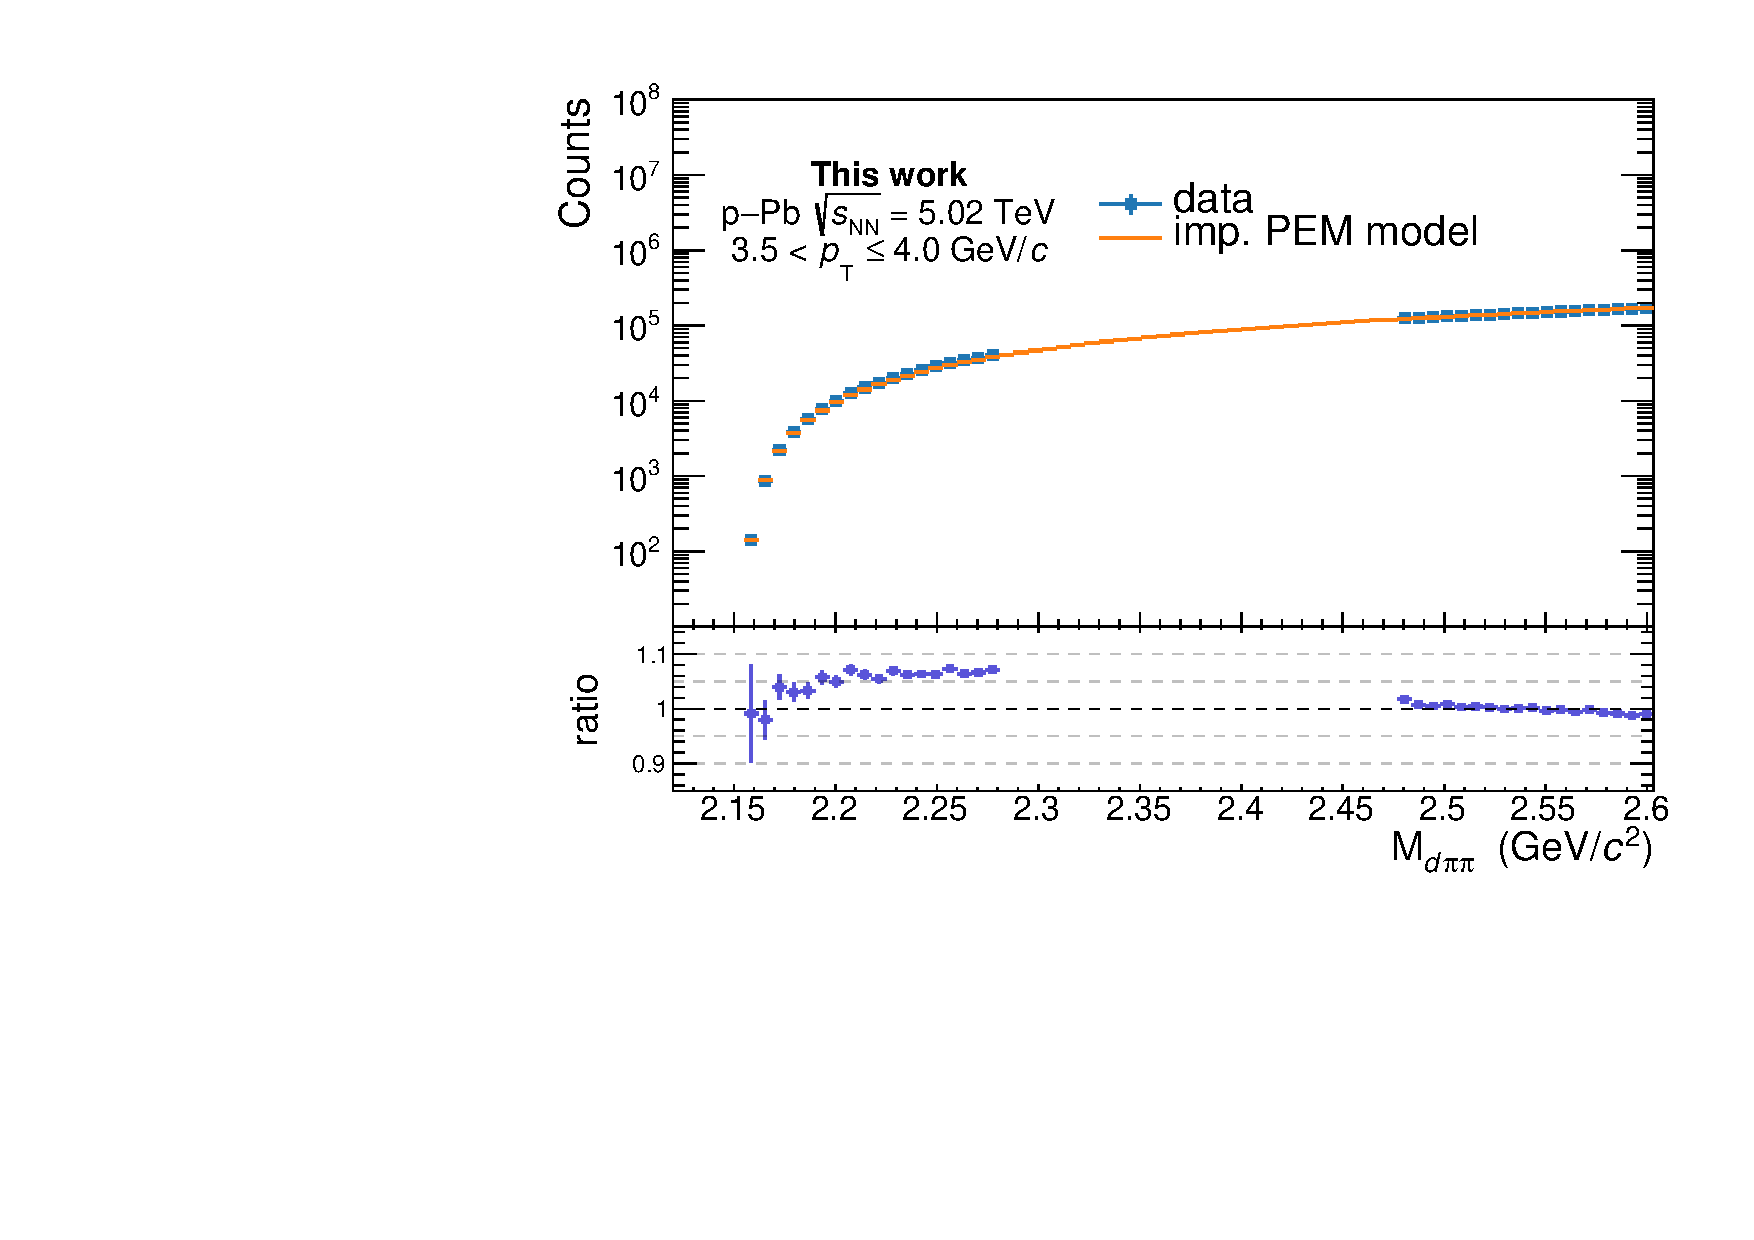
\includegraphics[width=\linewidth]{gfx/appendix/impem/can_blindPEMimp7}
  \caption{}
\end{subfigure}
\caption{PEM model compared with \minv, outside the region of interest. In the lower pad the data/model ratio is reported. Panel (a) shows the data-model comparison in the $3.0 < \pt \leq 3.5 \gevc$ interval, while Panels (b) in the $3.5 < \pt \leq 4.0 \gevc$ interval.}
\end{figure}
\clearpage

\chapter{Appendix} \label{app:bs}

This appendix is devoted to the illustration of the additional plot related to the background subtraction
described in Section~\ref{sec:backsub}.

%
%
\section{Data-model comparison in the RoI} \label{app:bs1}

In the following the full list of figures related to the data-model \ -- i.e. improved PEM model -- \
comparison, in the region of interest, is presented. 
This study has been performed in the $0.0 - 4.0\ \gevc$ transverse momentum interval,
since for higher \pt the \ds production is expected to be negligible. 

\begin{figure}[!h]
\begin{subfigure}{.5\textwidth}
  \centering
  \captionsetup{justification=centering}
  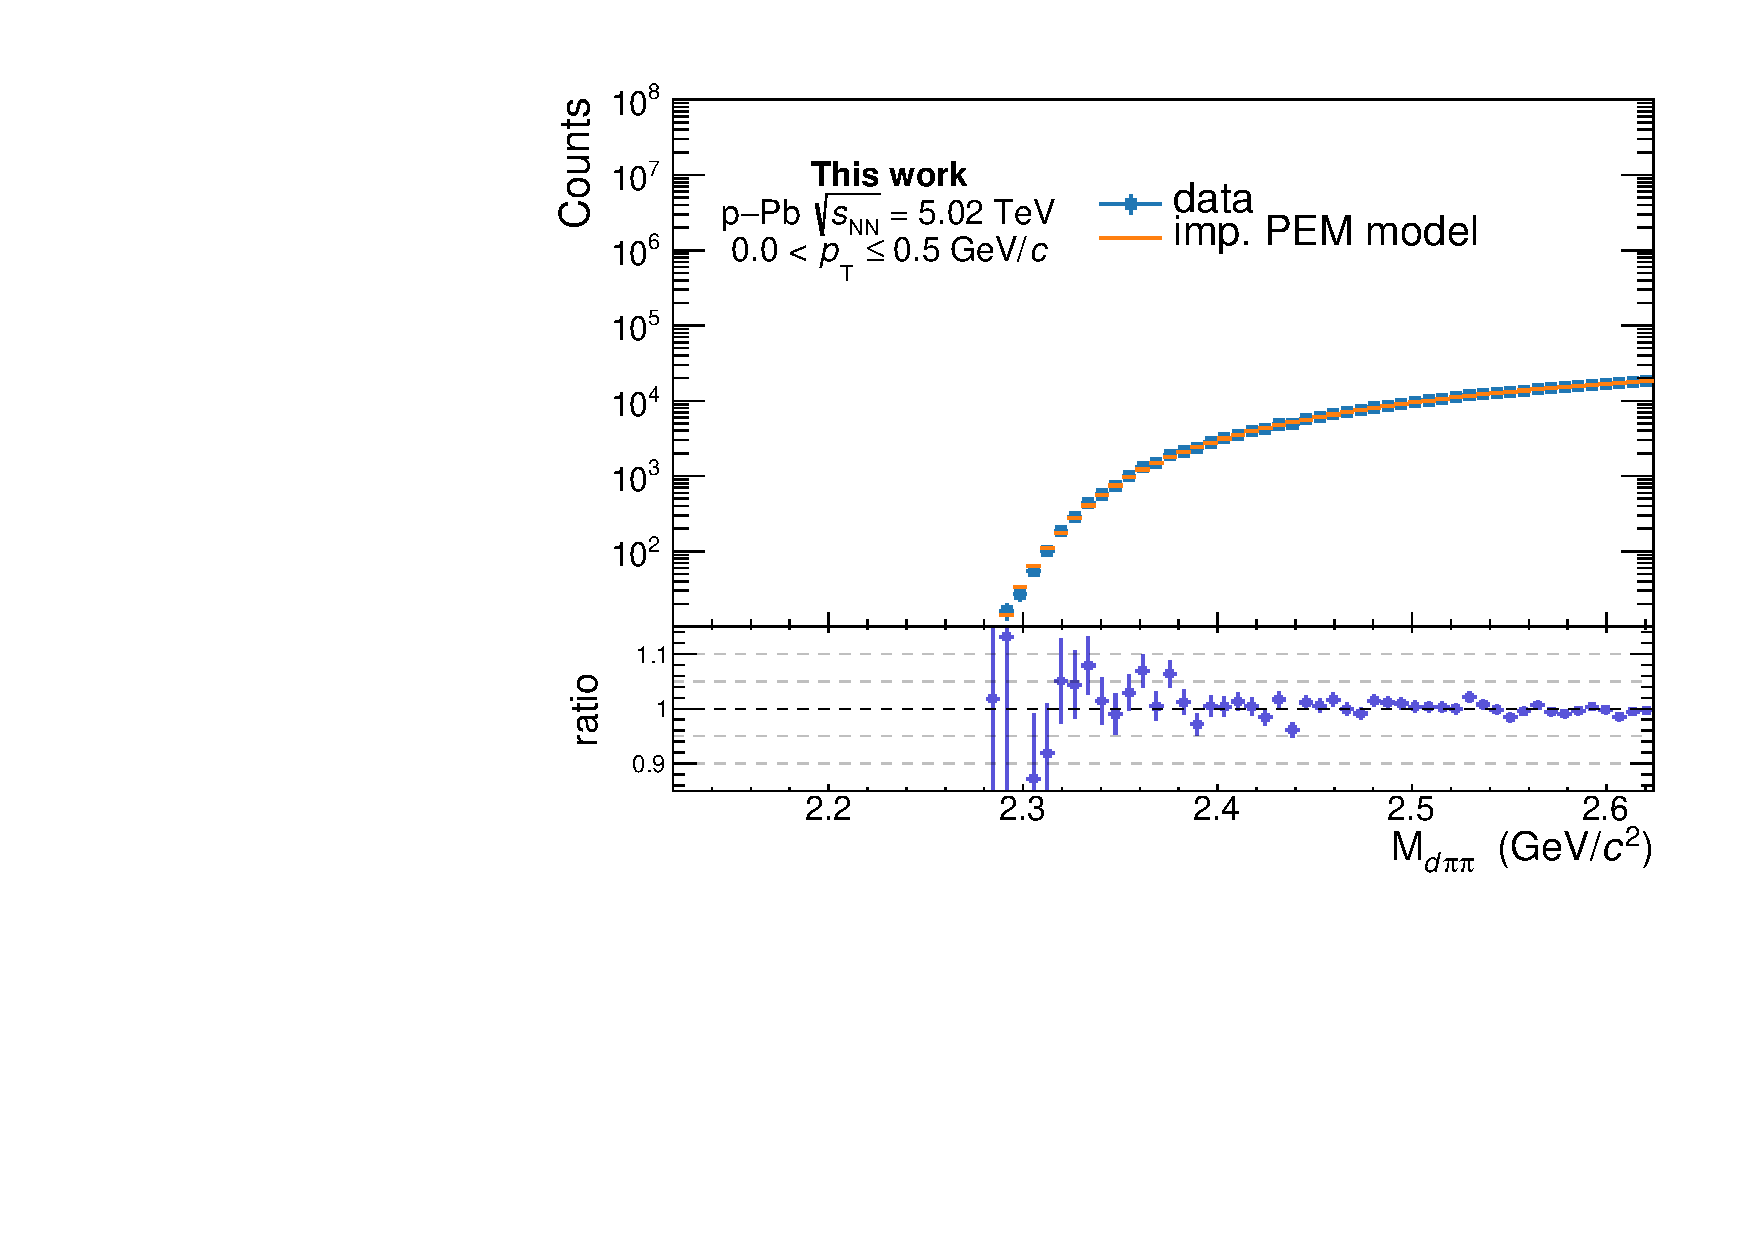
\includegraphics[width=\linewidth]{gfx/appendix/backsub/can_unblind0}
  \caption{}
\end{subfigure}%
\begin{subfigure}{.5\textwidth}
  \centering
  \captionsetup{justification=centering}
  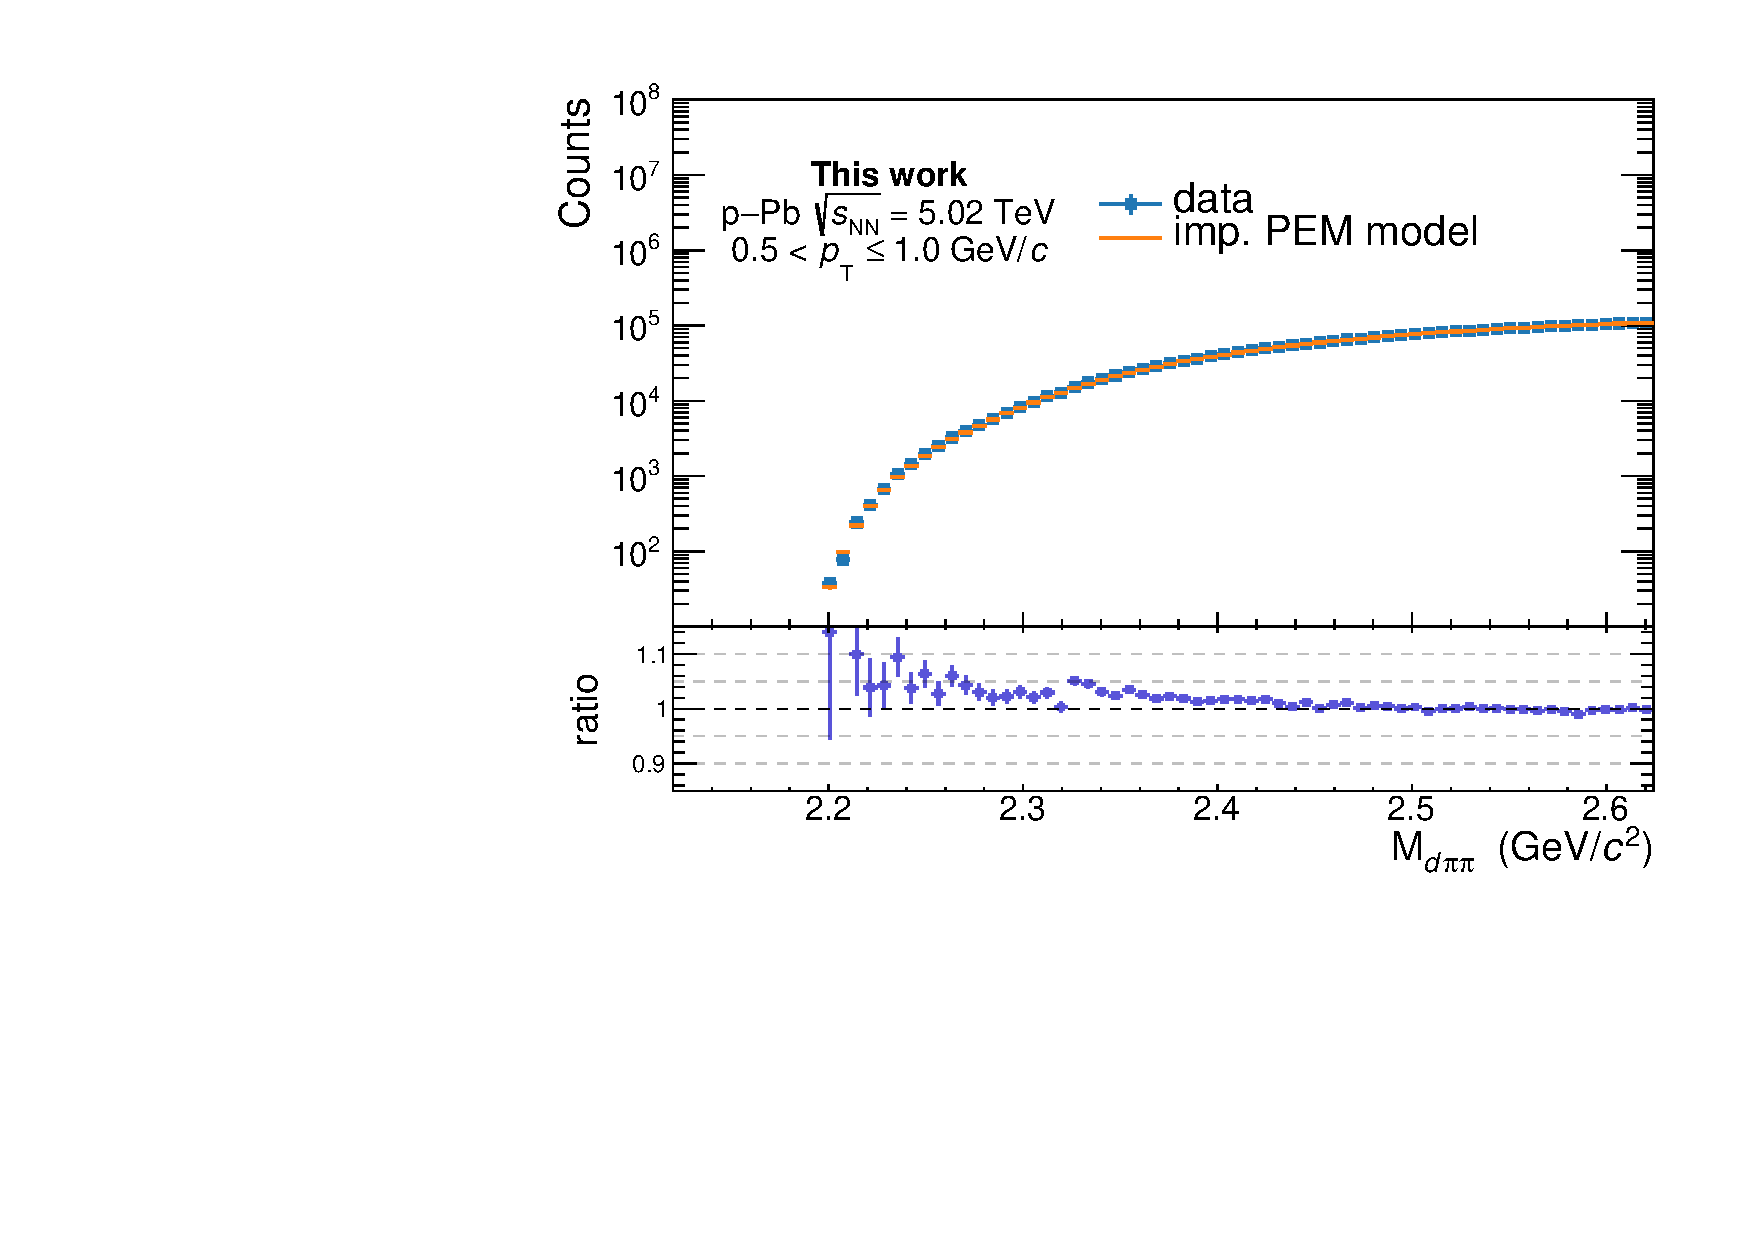
\includegraphics[width=\linewidth]{gfx/appendix/backsub/can_unblind1}
  \caption{}
\end{subfigure}
\begin{subfigure}{.5\textwidth}
  \centering
  \captionsetup{justification=centering}
  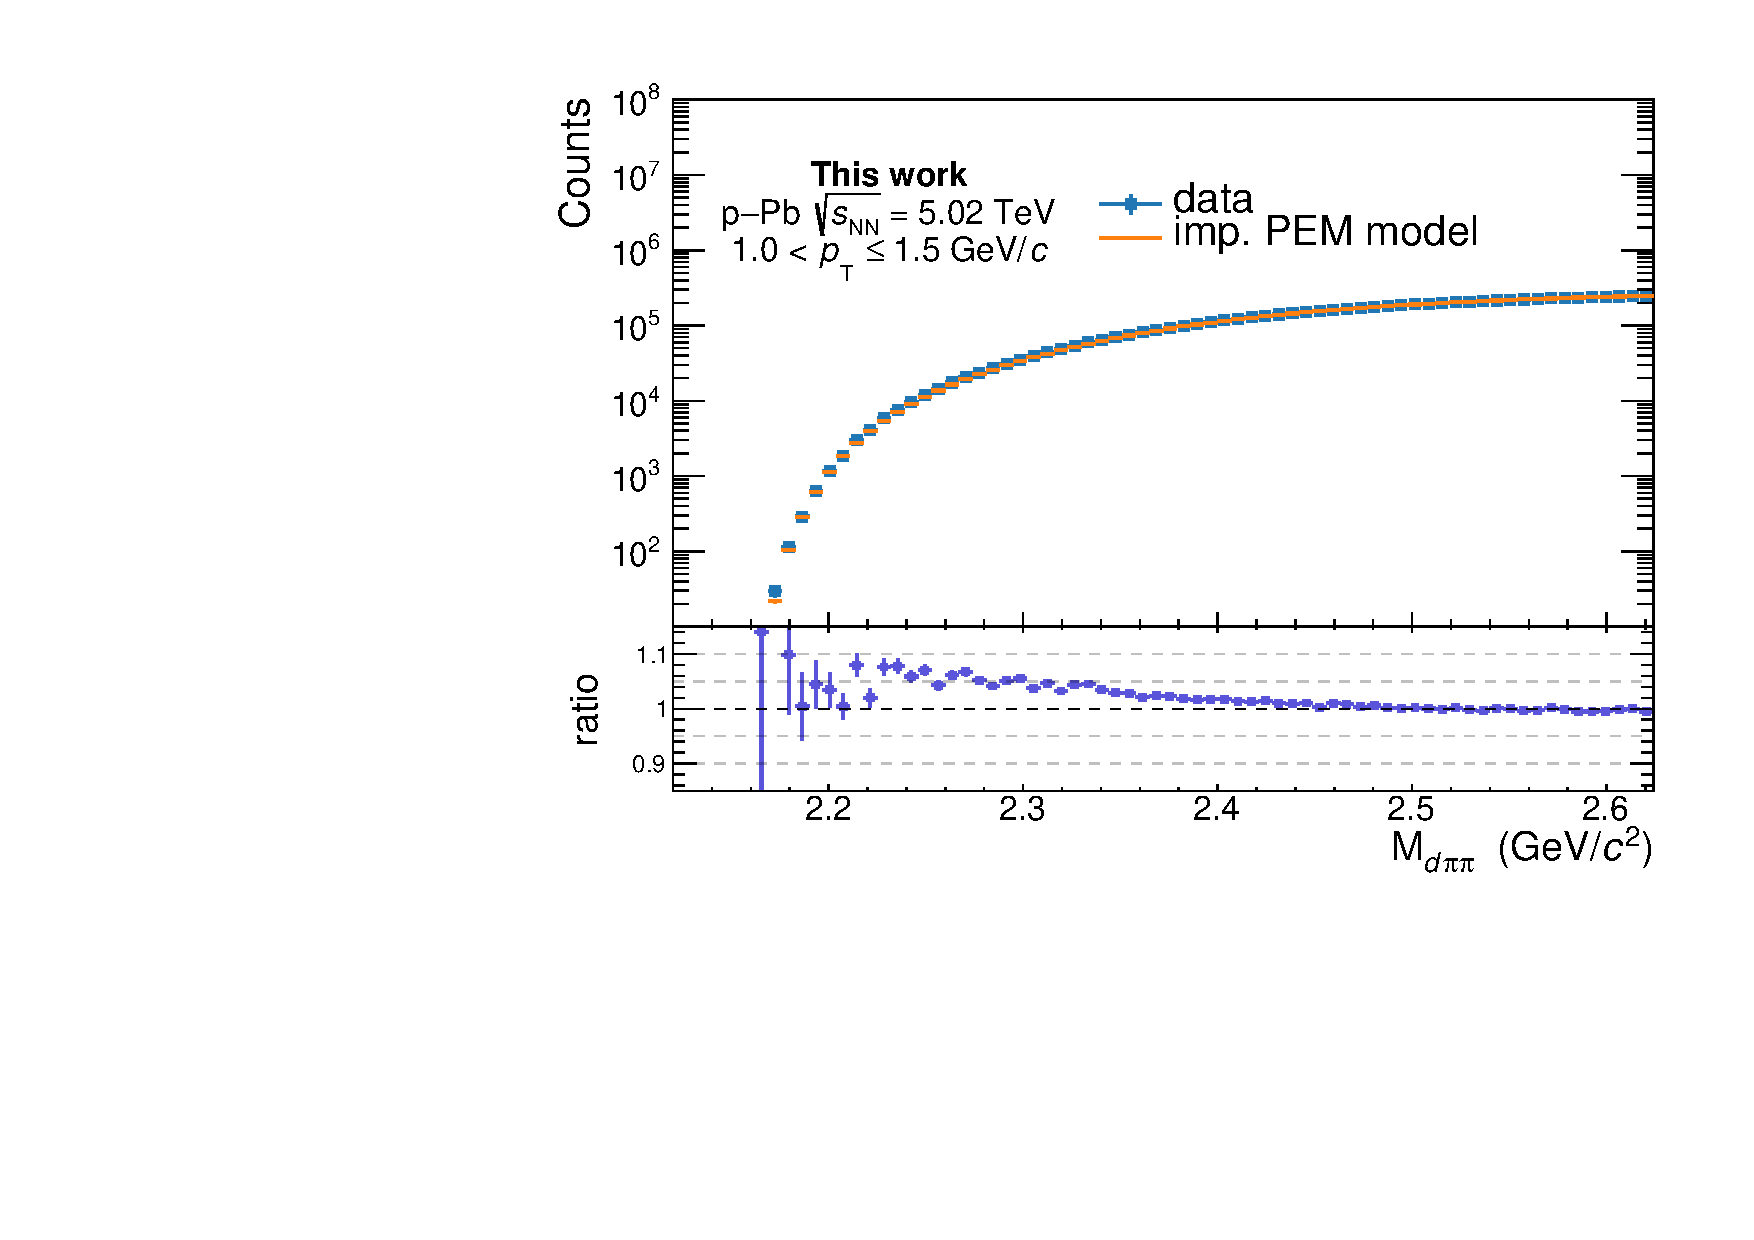
\includegraphics[width=\linewidth]{gfx/appendix/backsub/can_unblind2}
  \caption{}
\end{subfigure}%
\begin{subfigure}{.5\textwidth}
  \centering
  \captionsetup{justification=centering}
  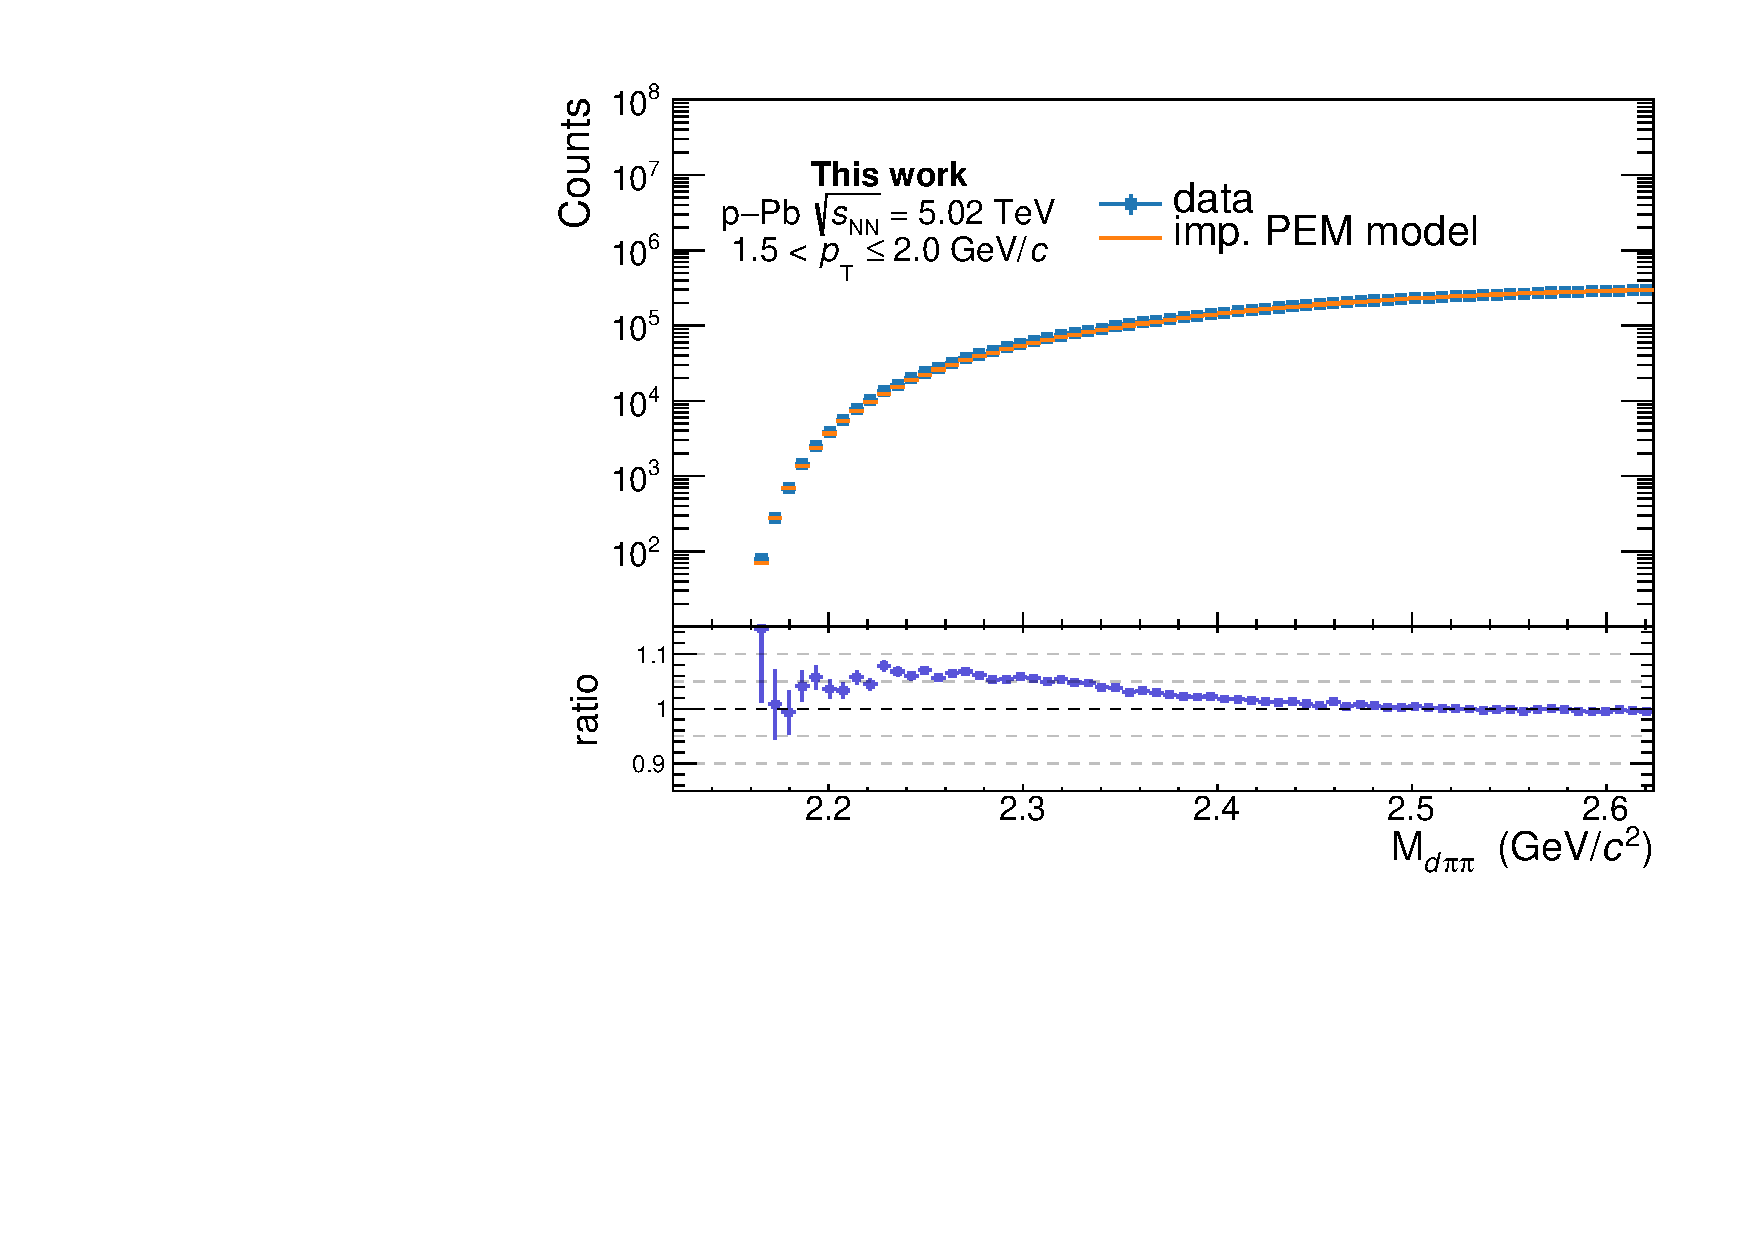
\includegraphics[width=\linewidth]{gfx/appendix/backsub/can_unblind3}
  \caption{}
\end{subfigure}
\caption{PEM model compared with \minv in the region of interest. In the lower pad the data/model ratio is reported. Panel (a) shows the data-model comparison in the $0.0 < \pt \leq 0.5 \ \gevc$ interval, while Panels (b), (c) and (d) in the $0.5 < \pt \leq 1.0 \ \gevc$, $1.0 < \pt \leq 1.5 \ \gevc$ and $1.5 < \pt \leq 2.0 \ \gevc$ intervals respectively.}
\end{figure}

\begin{figure}[htb]
\begin{subfigure}{.5\textwidth}
  \centering
  \captionsetup{justification=centering}
  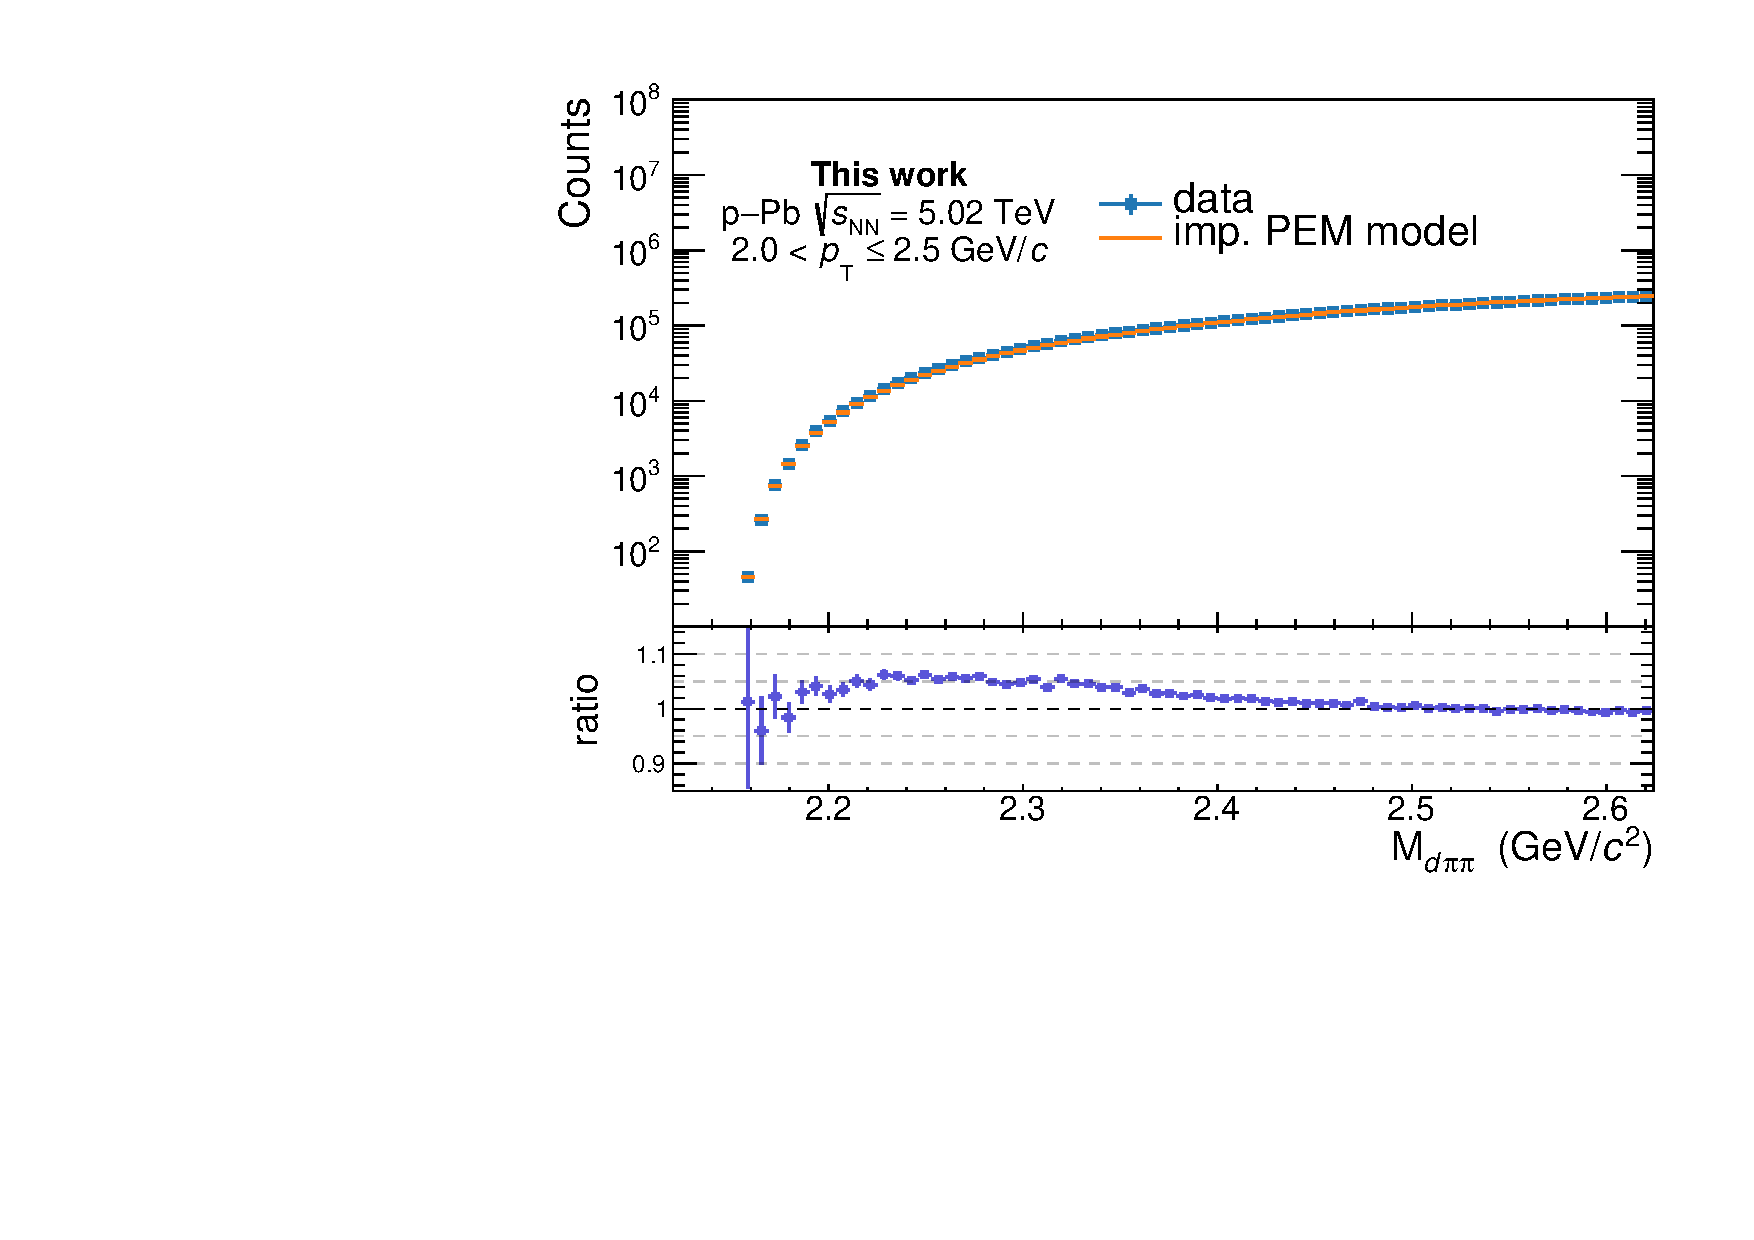
\includegraphics[width=\linewidth]{gfx/appendix/backsub/can_unblind4}
  \caption{}
\end{subfigure}%
\begin{subfigure}{.5\textwidth}
  \centering
  \captionsetup{justification=centering}
  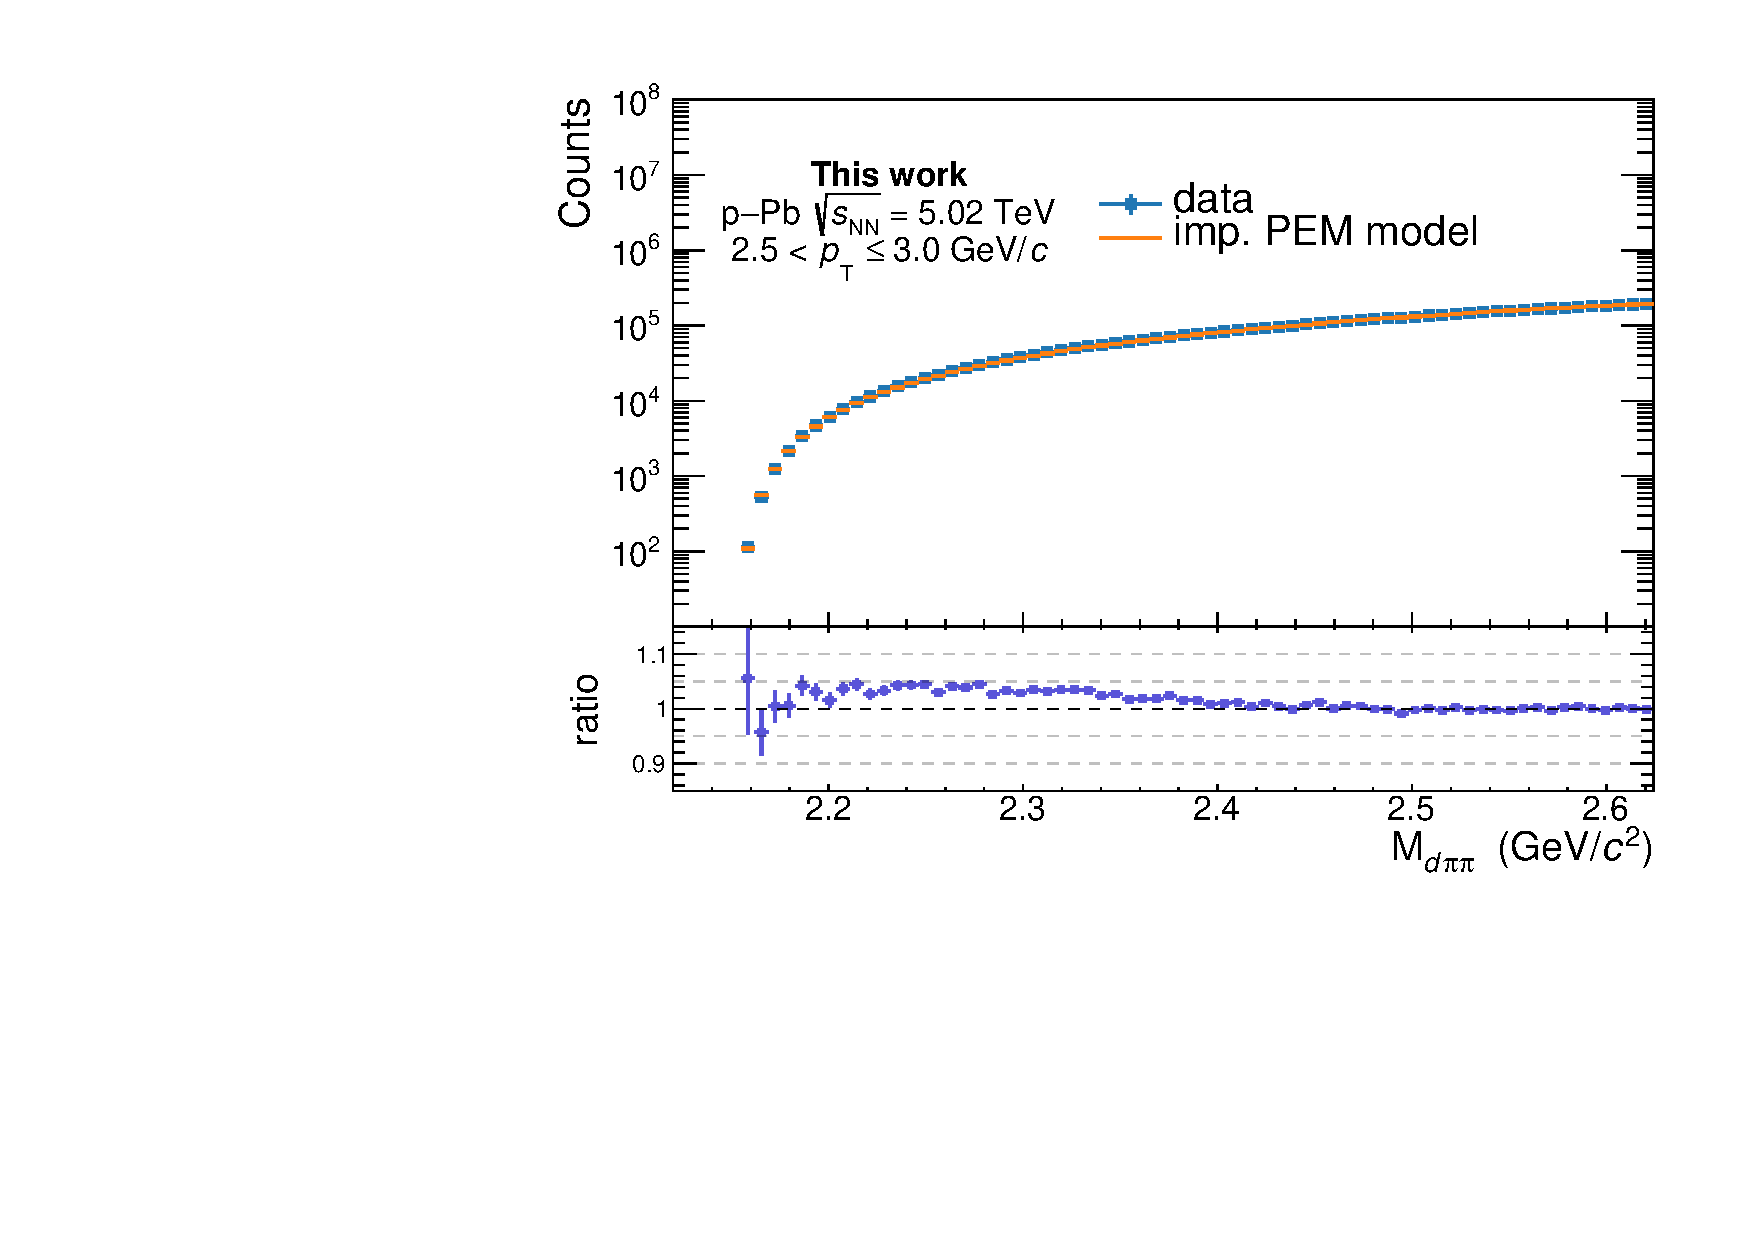
\includegraphics[width=\linewidth]{gfx/appendix/backsub/can_unblind5}
  \caption{}
\end{subfigure}
\begin{subfigure}{.5\textwidth}
  \centering
  \captionsetup{justification=centering}
  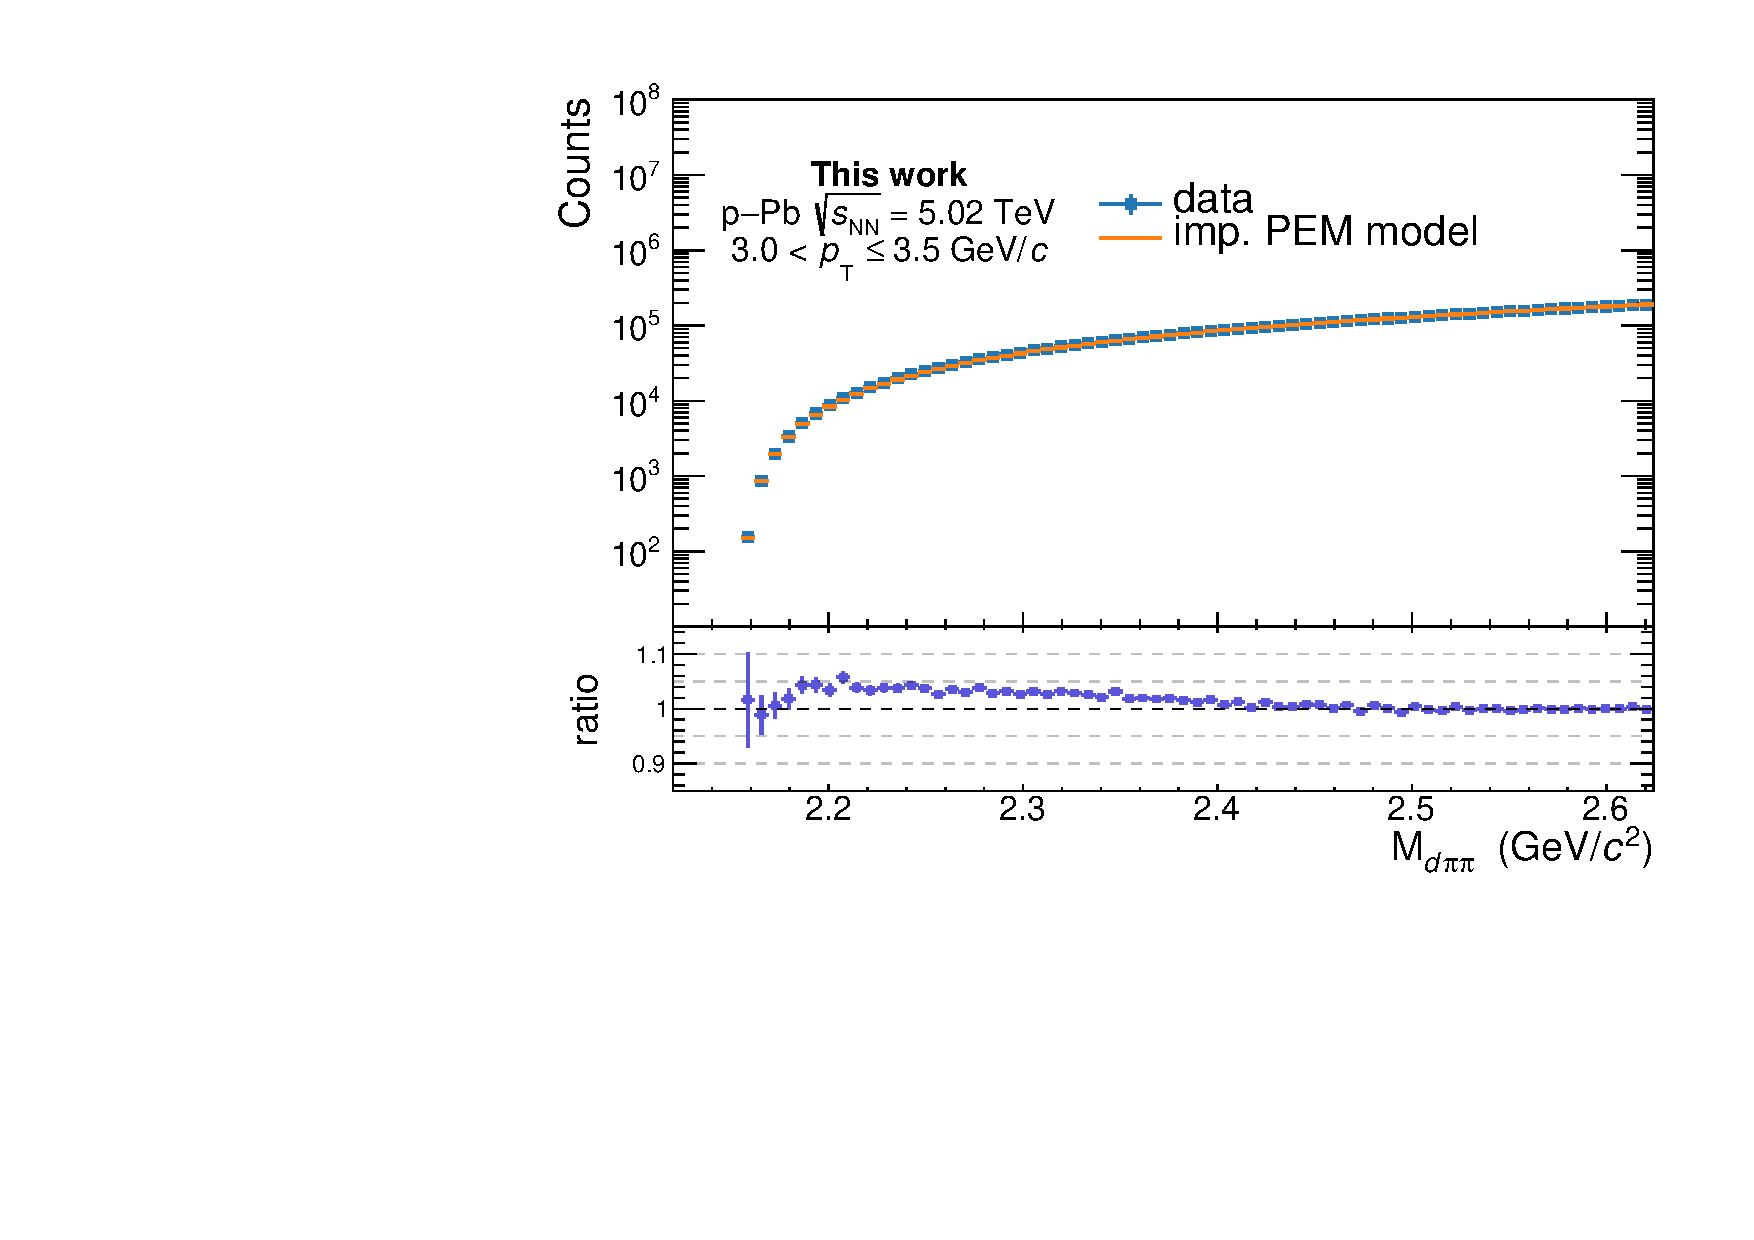
\includegraphics[width=\linewidth]{gfx/appendix/backsub/can_unblind6}
  \caption{}
\end{subfigure}%
\begin{subfigure}{.5\textwidth}
  \centering
  \captionsetup{justification=centering}
  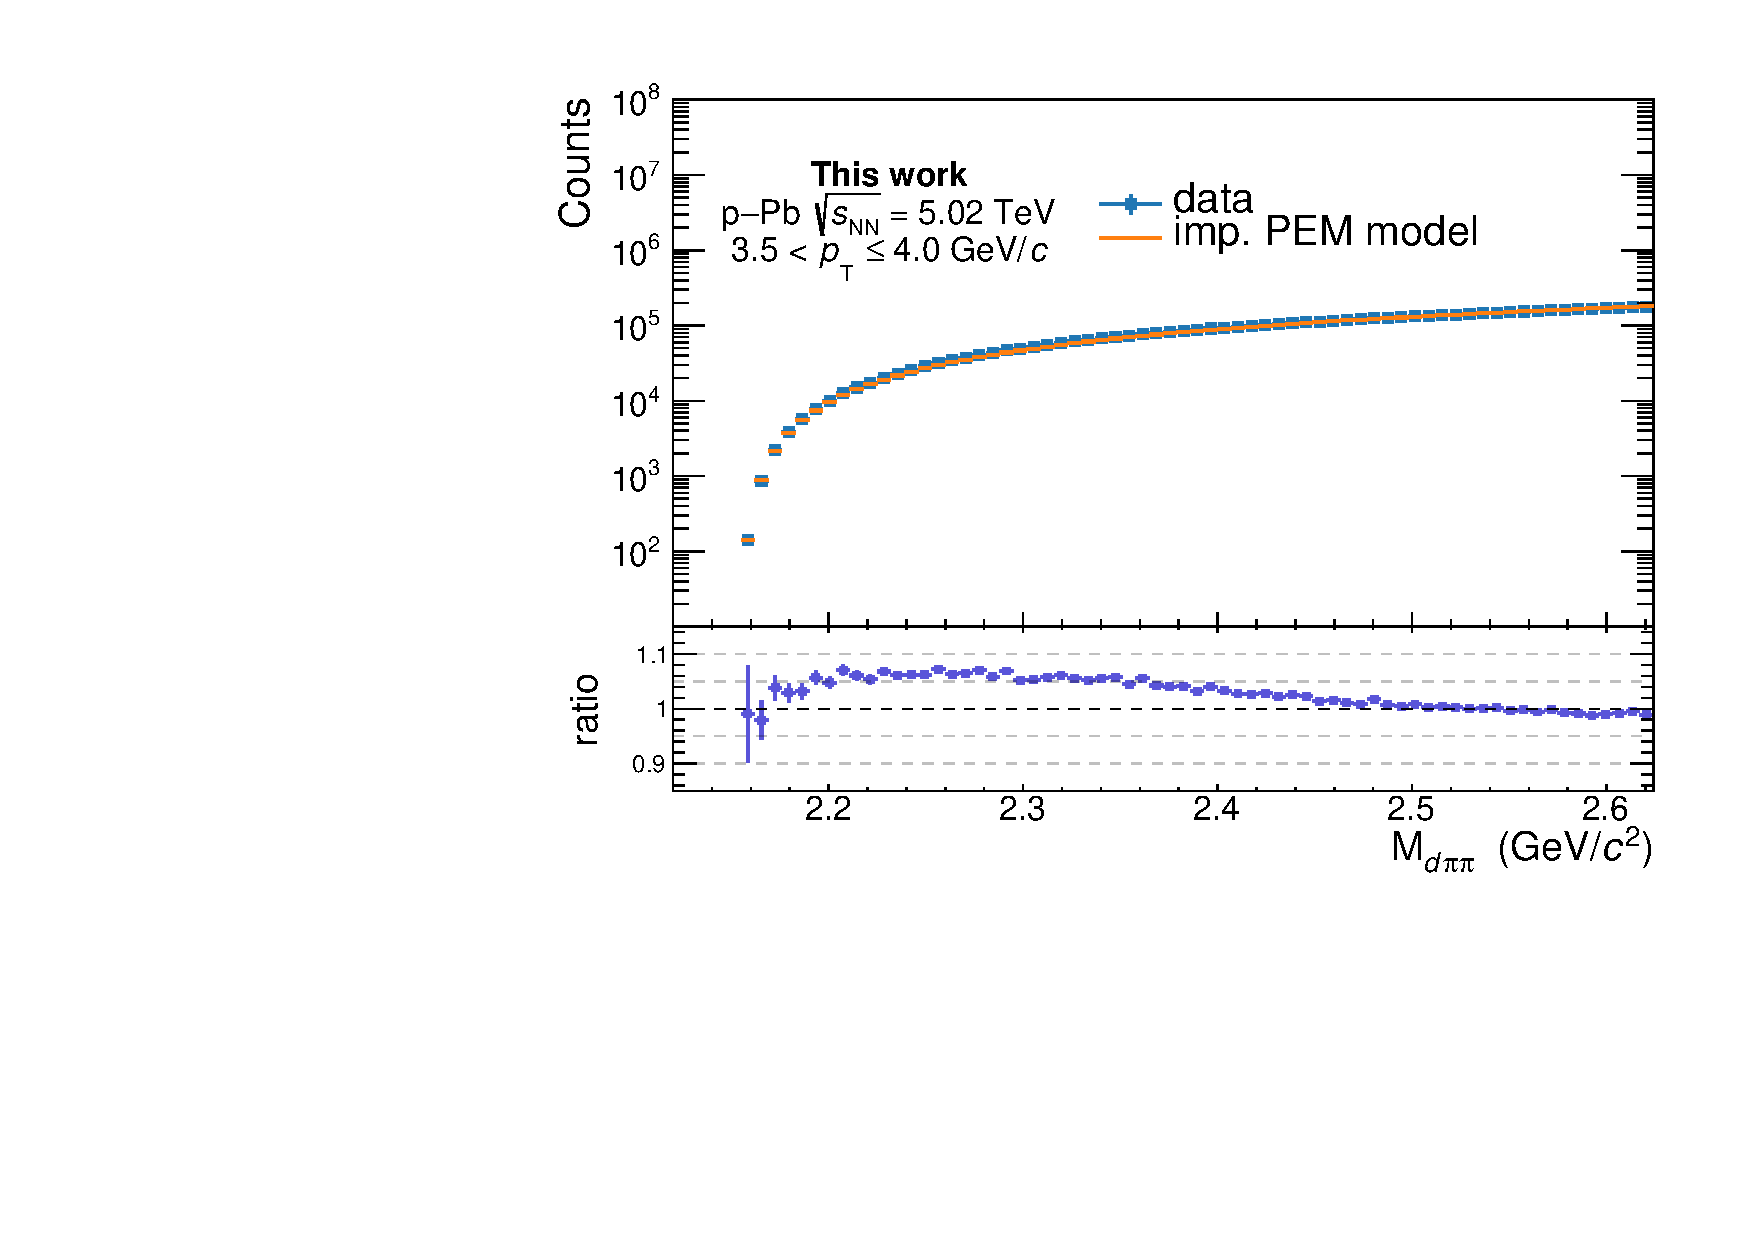
\includegraphics[width=\linewidth]{gfx/appendix/backsub/can_unblind7}
  \caption{}
\end{subfigure}
\caption{PEM model compared with \minv, in the region of interest. In the lower pad the data/model ratio is reported. Panel (a) shows the data-model comparison in the $2.0 < \pt \leq 2.5\ \gevc$ interval, while Panels (b), (c) and (d) in the $2.5 < \pt \leq 3.0\ \gevc$, $3.0 < \pt \leq 3.5\ \gevc$ and $3.5 < \pt \leq 4.0\ \gevc$ intervals respectively.}
\end{figure}
\clearpage

%
%
\section{Background subtraction} \label{app:bs2}

In the following the full list of figures related to the background subtraction is presented.
The background subtraction was performed, following the procedure described in Section~\ref{sec:backsub},
in the $0.5 - 4.0\ \gevc$ transverse momentum interval, since for higher \pt the \ds production is
expected to be negligible.
\begin{figure} [htb]
    \centering
    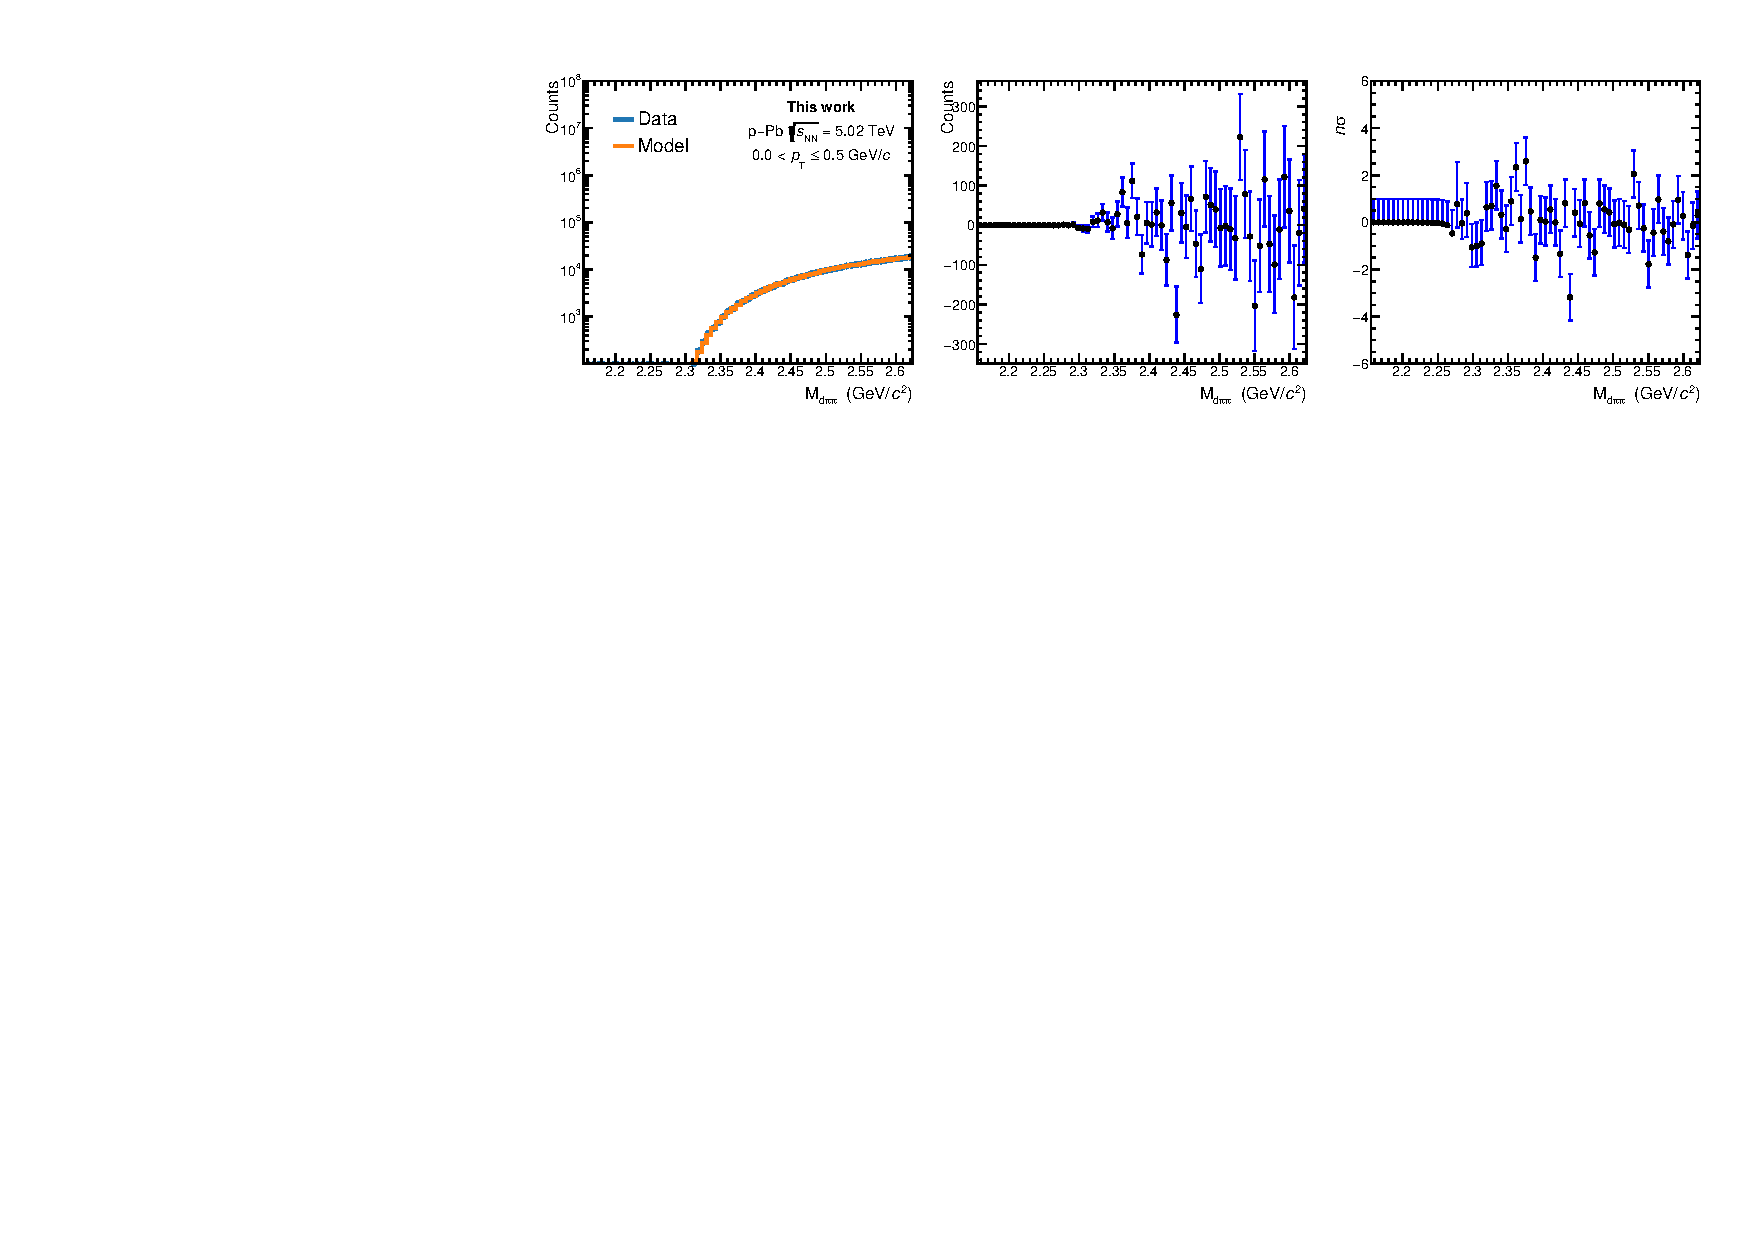
\includegraphics[width=\textwidth]{gfx/appendix/backsub/canvas0}
    \caption{Left panel shows the background model compared with \minv, in the $0.0 < \pt \leq 0.5$ \gevc interval. In the central panel the residual discrepancies are fitted with a constant function, while in the right panel the pull distribution is reported.}
    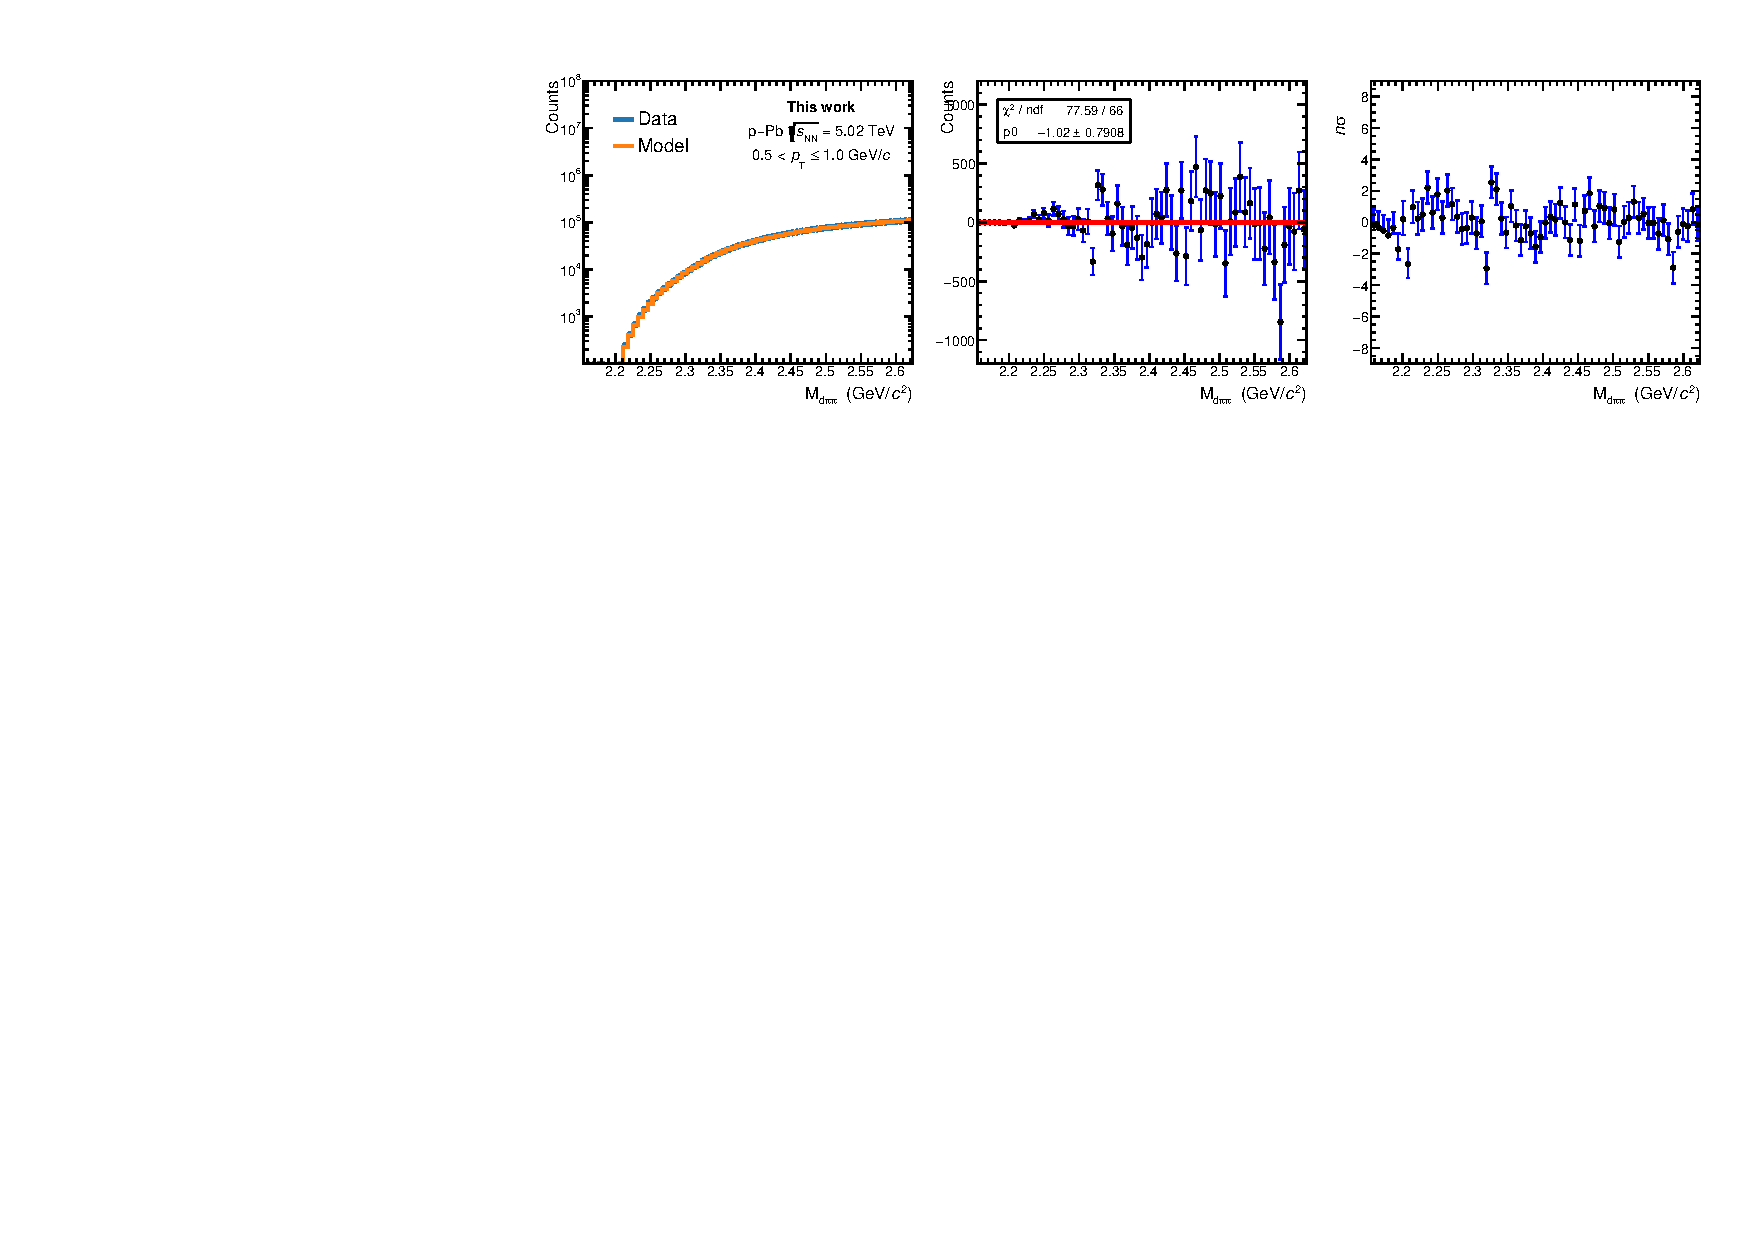
\includegraphics[width=\textwidth]{gfx/appendix/backsub/canvas1}
    \caption{Left panel shows the background model compared with \minv, in the $0.5 < \pt \leq 1.0$ \gevc interval. In the central panel the residual discrepancies are fitted with a constant function, while in the right panel the pull distribution is reported.}
    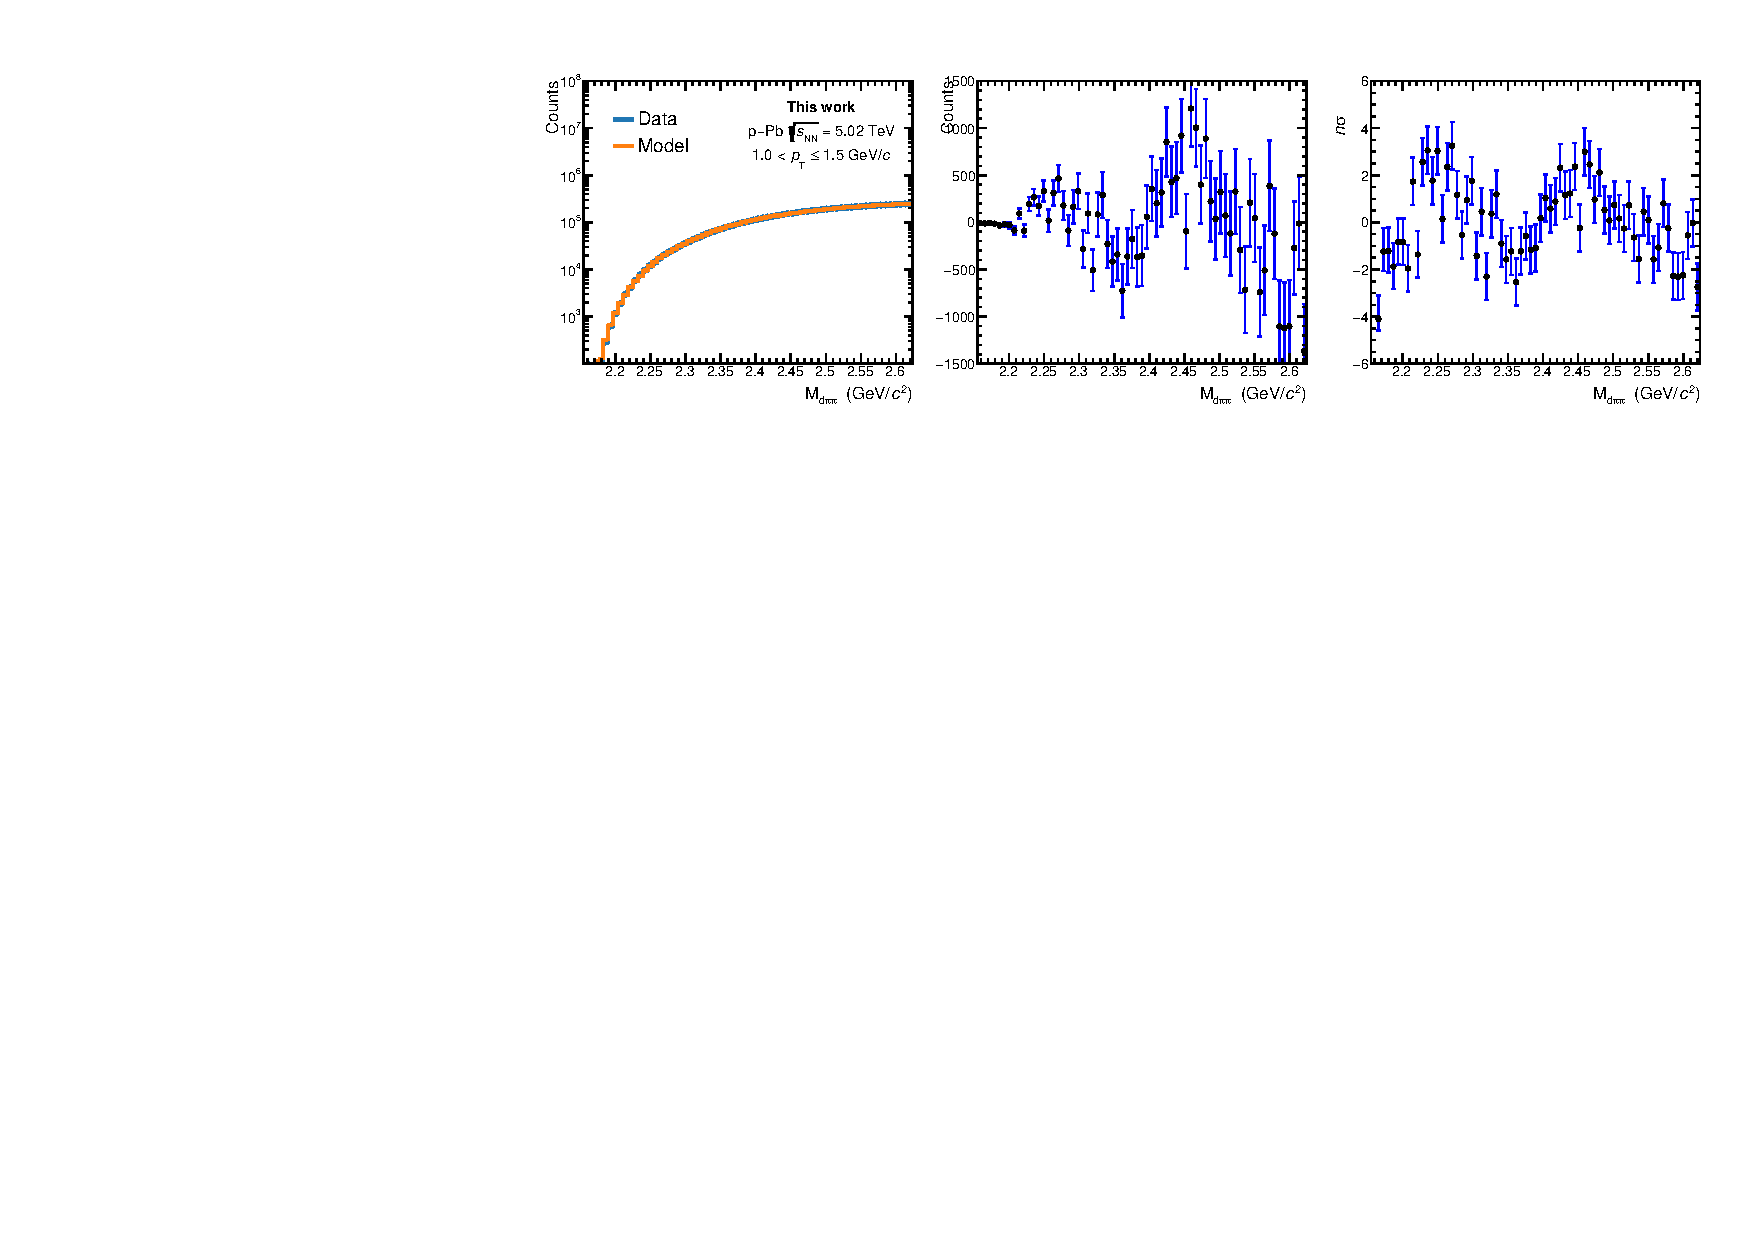
\includegraphics[width=\textwidth]{gfx/appendix/backsub/canvas2}
    \caption{Left panel shows the background model compared with \minv, in the $1.0 < \pt \leq 1.5$ \gevc interval. In the central panel the residual discrepancies are fitted with a constant function, while in the right panel the pull distribution is reported.}
\end{figure}

\begin{figure} [htb]
    \centering
    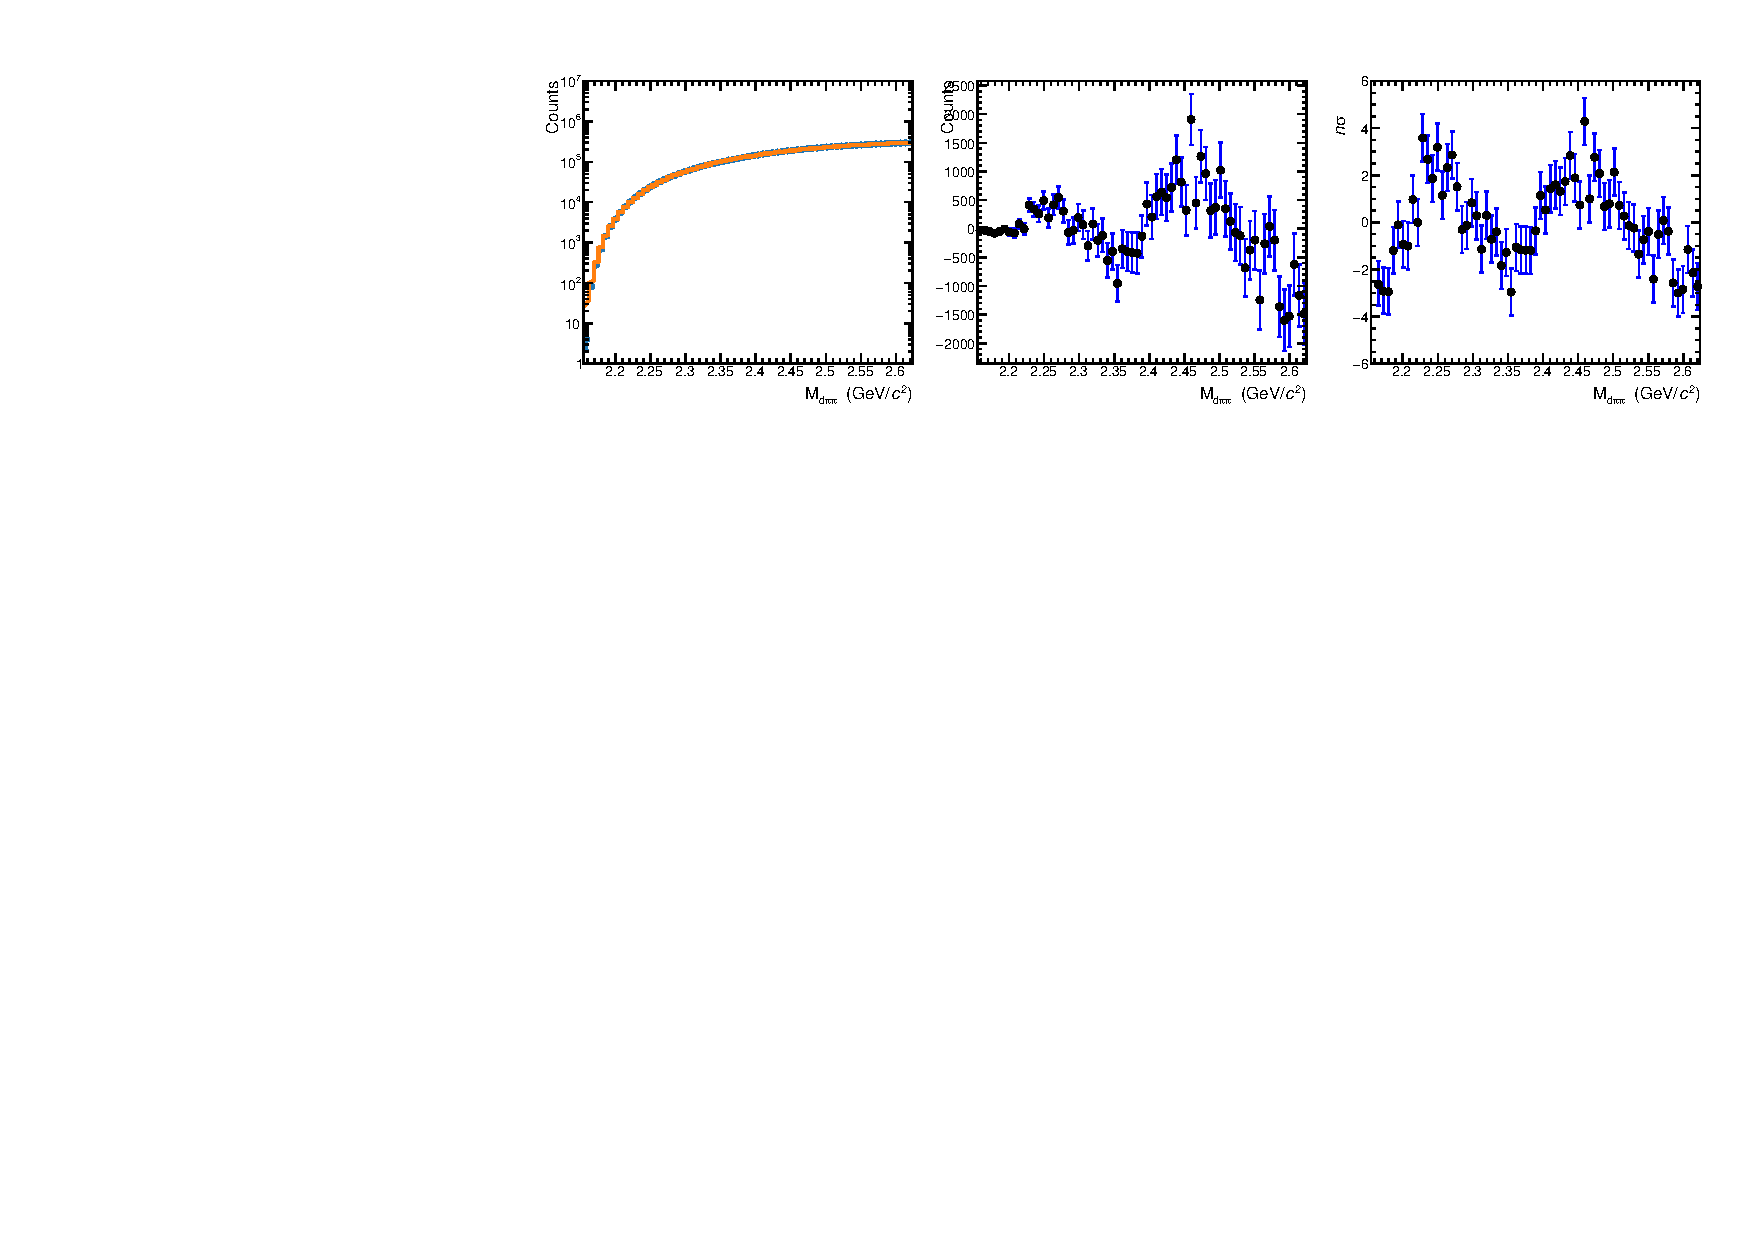
\includegraphics[width=\textwidth]{gfx/appendix/backsub/canvas3}
    \caption{Left panel shows the background model compared with \minv, in the $1.5 < \pt \leq 2.0$ \gevc interval. In the central panel the residual discrepancies are fitted with a constant function, while in the right panel the pull distribution is reported.}
    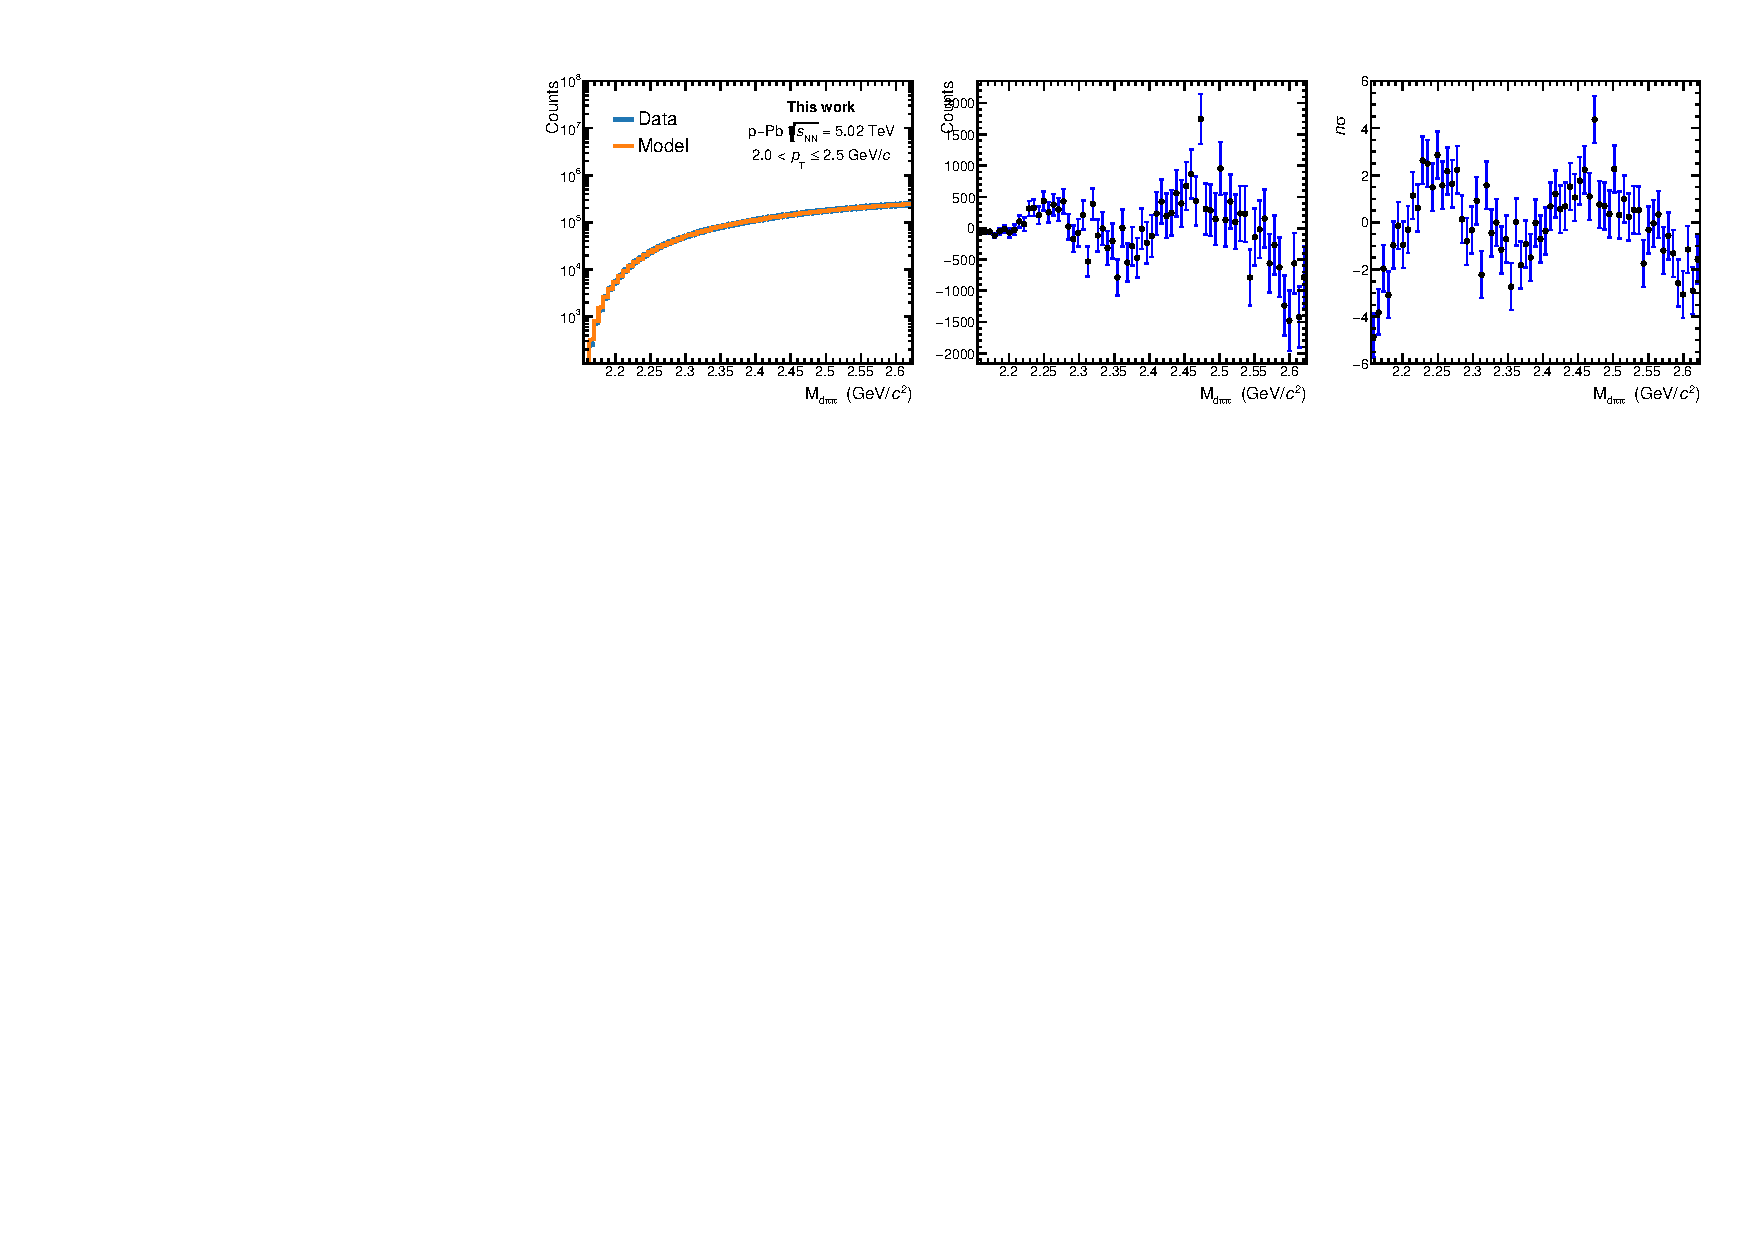
\includegraphics[width=\textwidth]{gfx/appendix/backsub/canvas4}
    \caption{Left panel shows the background model compared with \minv, in the $2.0 < \pt \leq 2.5$ \gevc interval. In the central panel the residual discrepancies are fitted with a constant function, while in the right panel the pull distribution is reported.}
    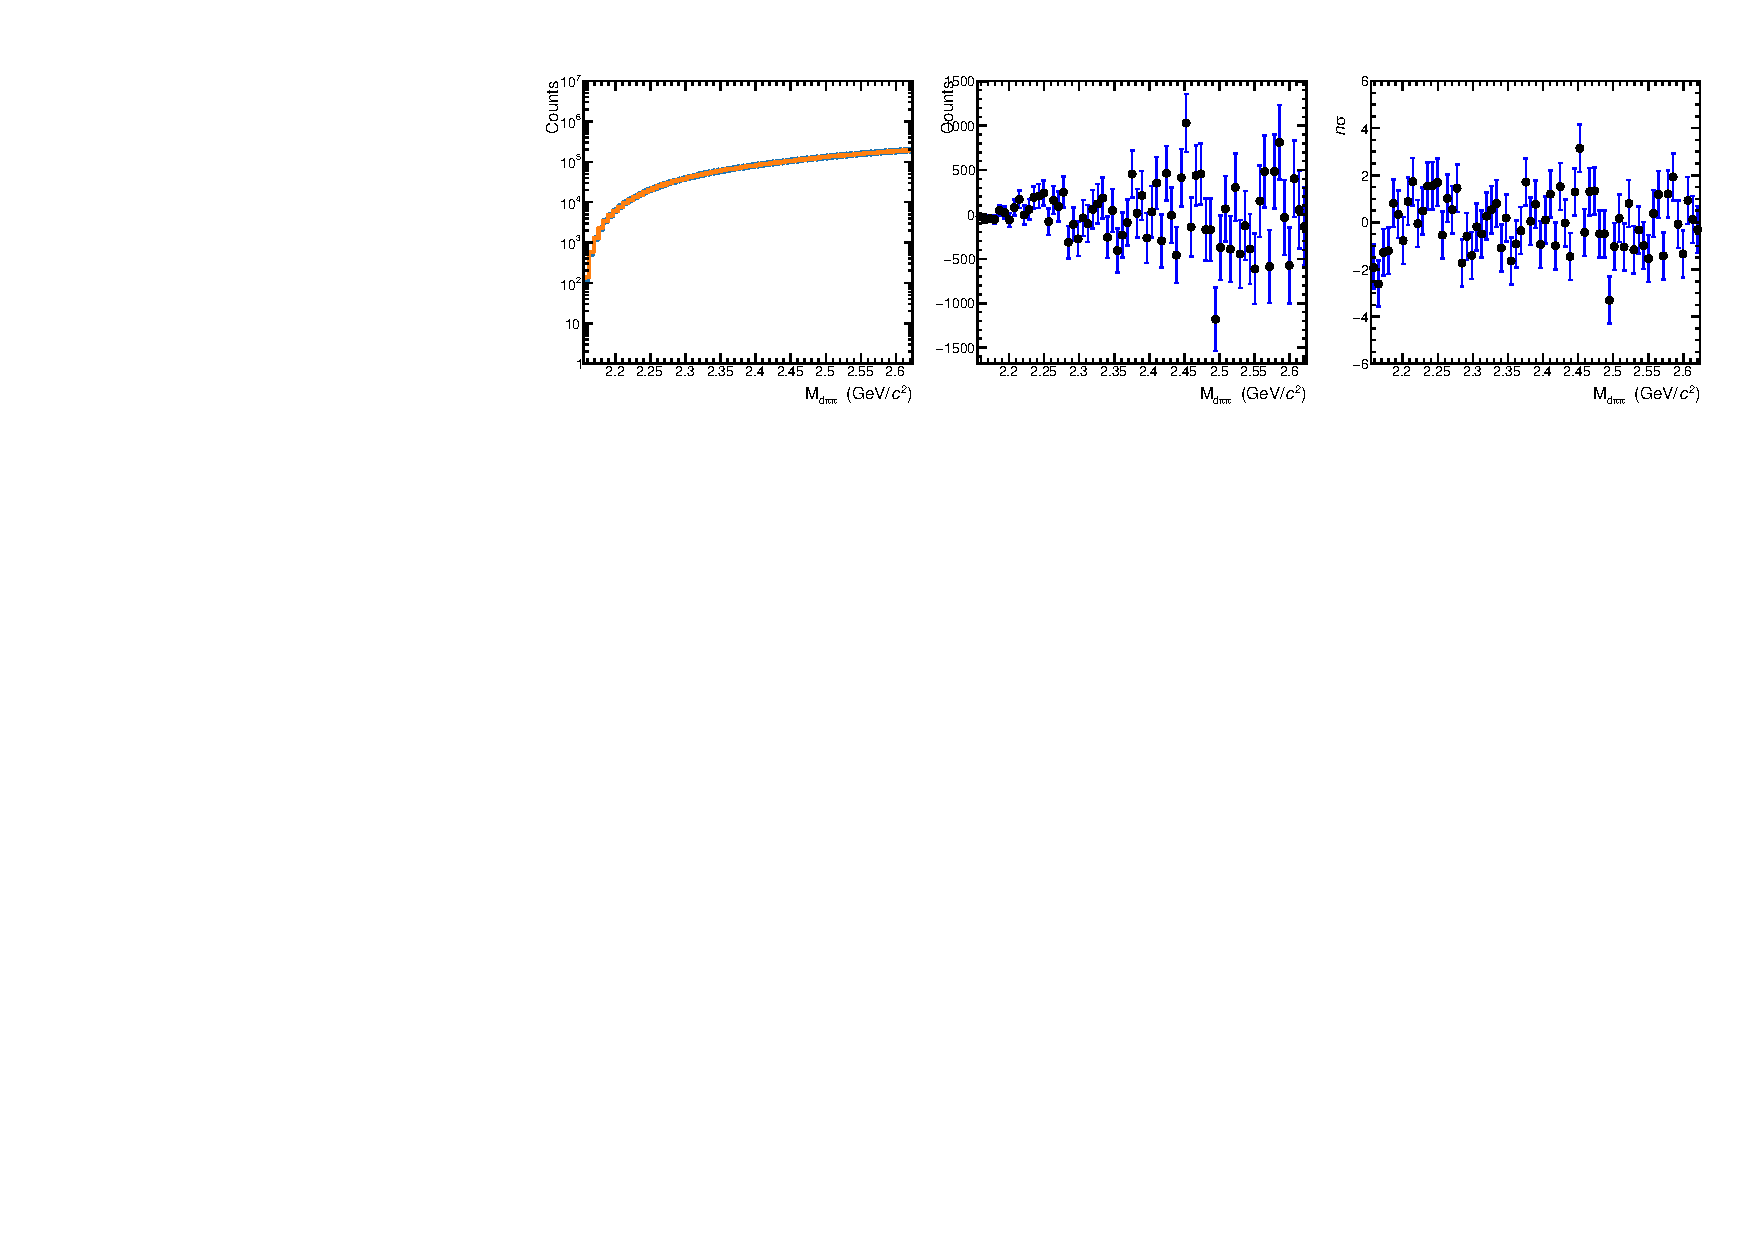
\includegraphics[width=\textwidth]{gfx/appendix/backsub/canvas5}
    \caption{Left panel shows the background model compared with \minv, in the $2.5 < \pt \leq 3.0$ \gevc interval. In the central panel the residual discrepancies are fitted with a constant function, while in the right panel the pull distribution is reported.}
        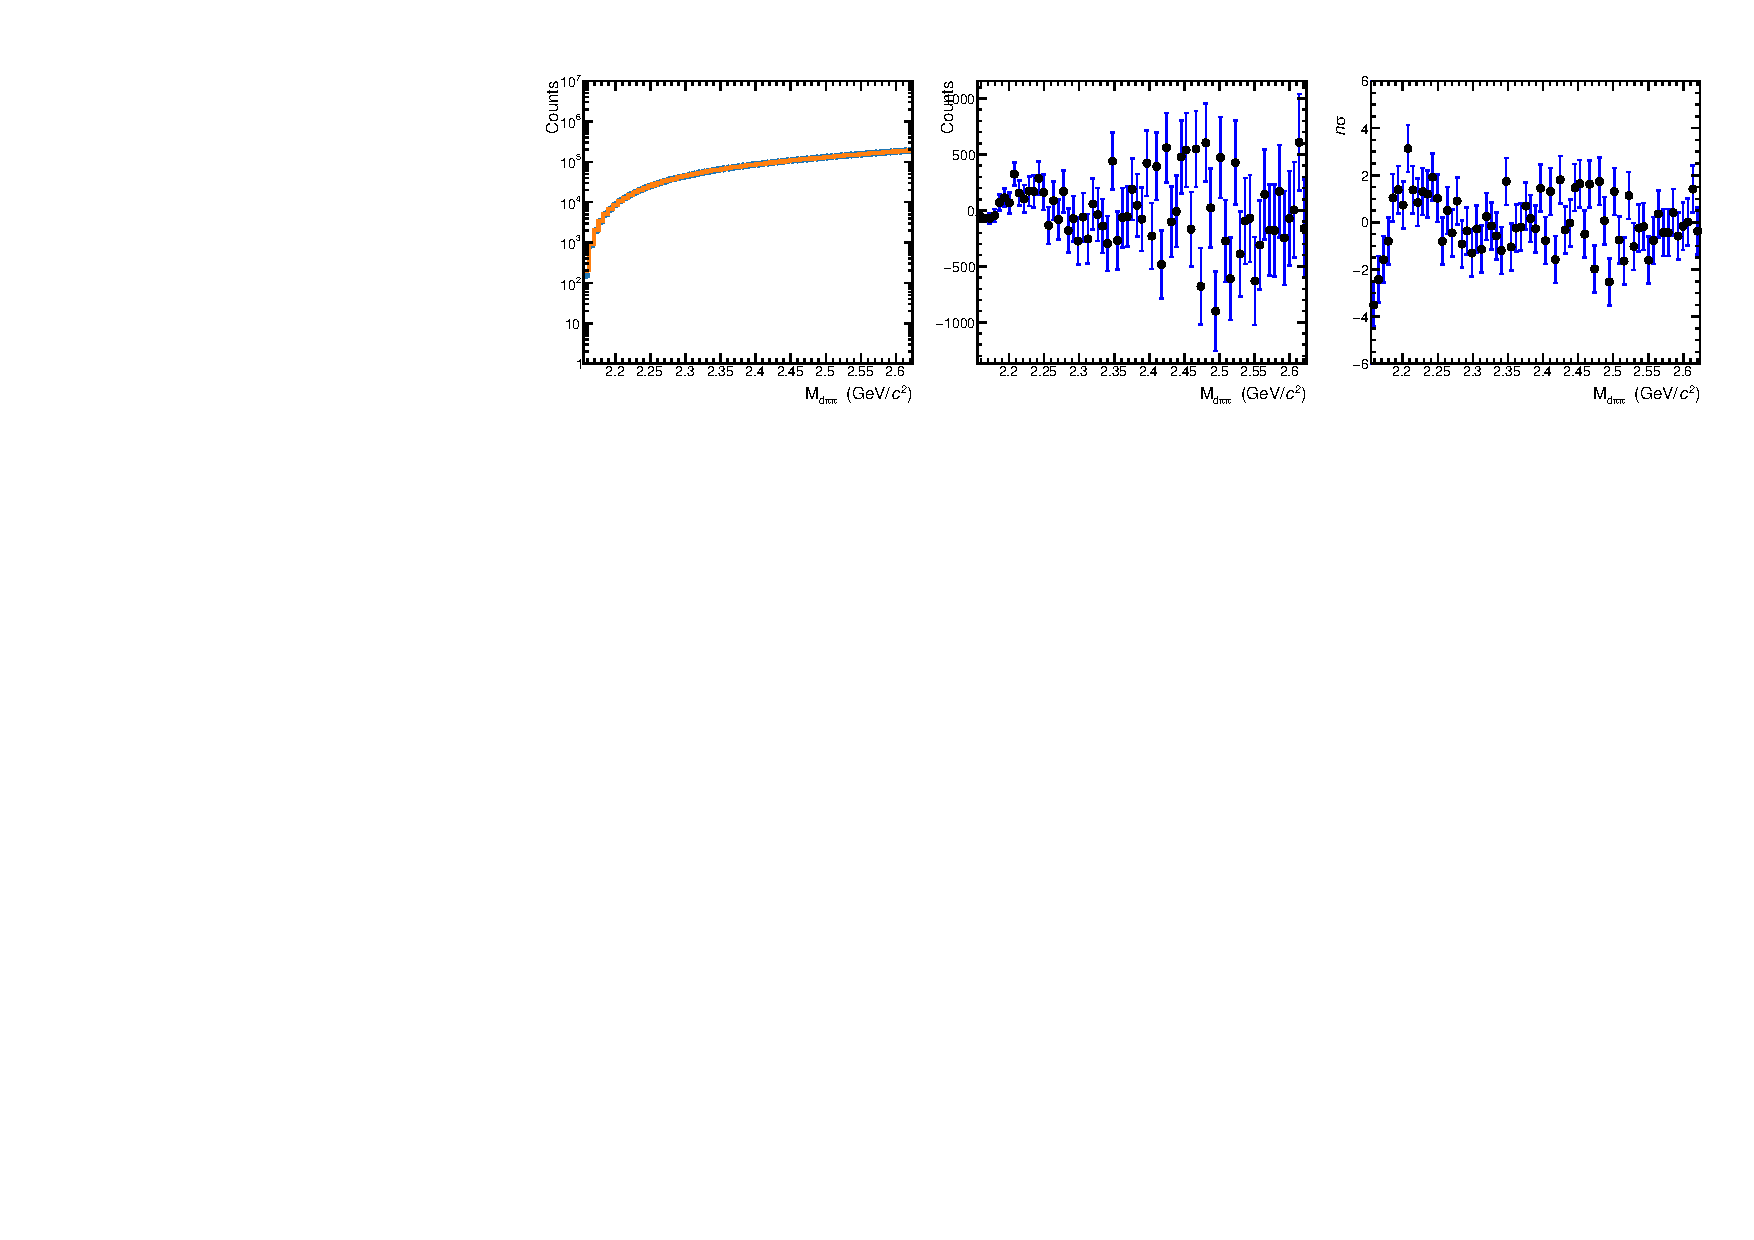
\includegraphics[width=\textwidth]{gfx/appendix/backsub/canvas6}
    \caption{Left panel shows the background model compared with \minv, in the $3.0 < \pt \leq 3.5$ \gevc interval. In the central panel the residual discrepancies are fitted with a constant function, while in the right panel the pull distribution is reported.}
\end{figure}

\begin{figure} [htb]
    \centering
    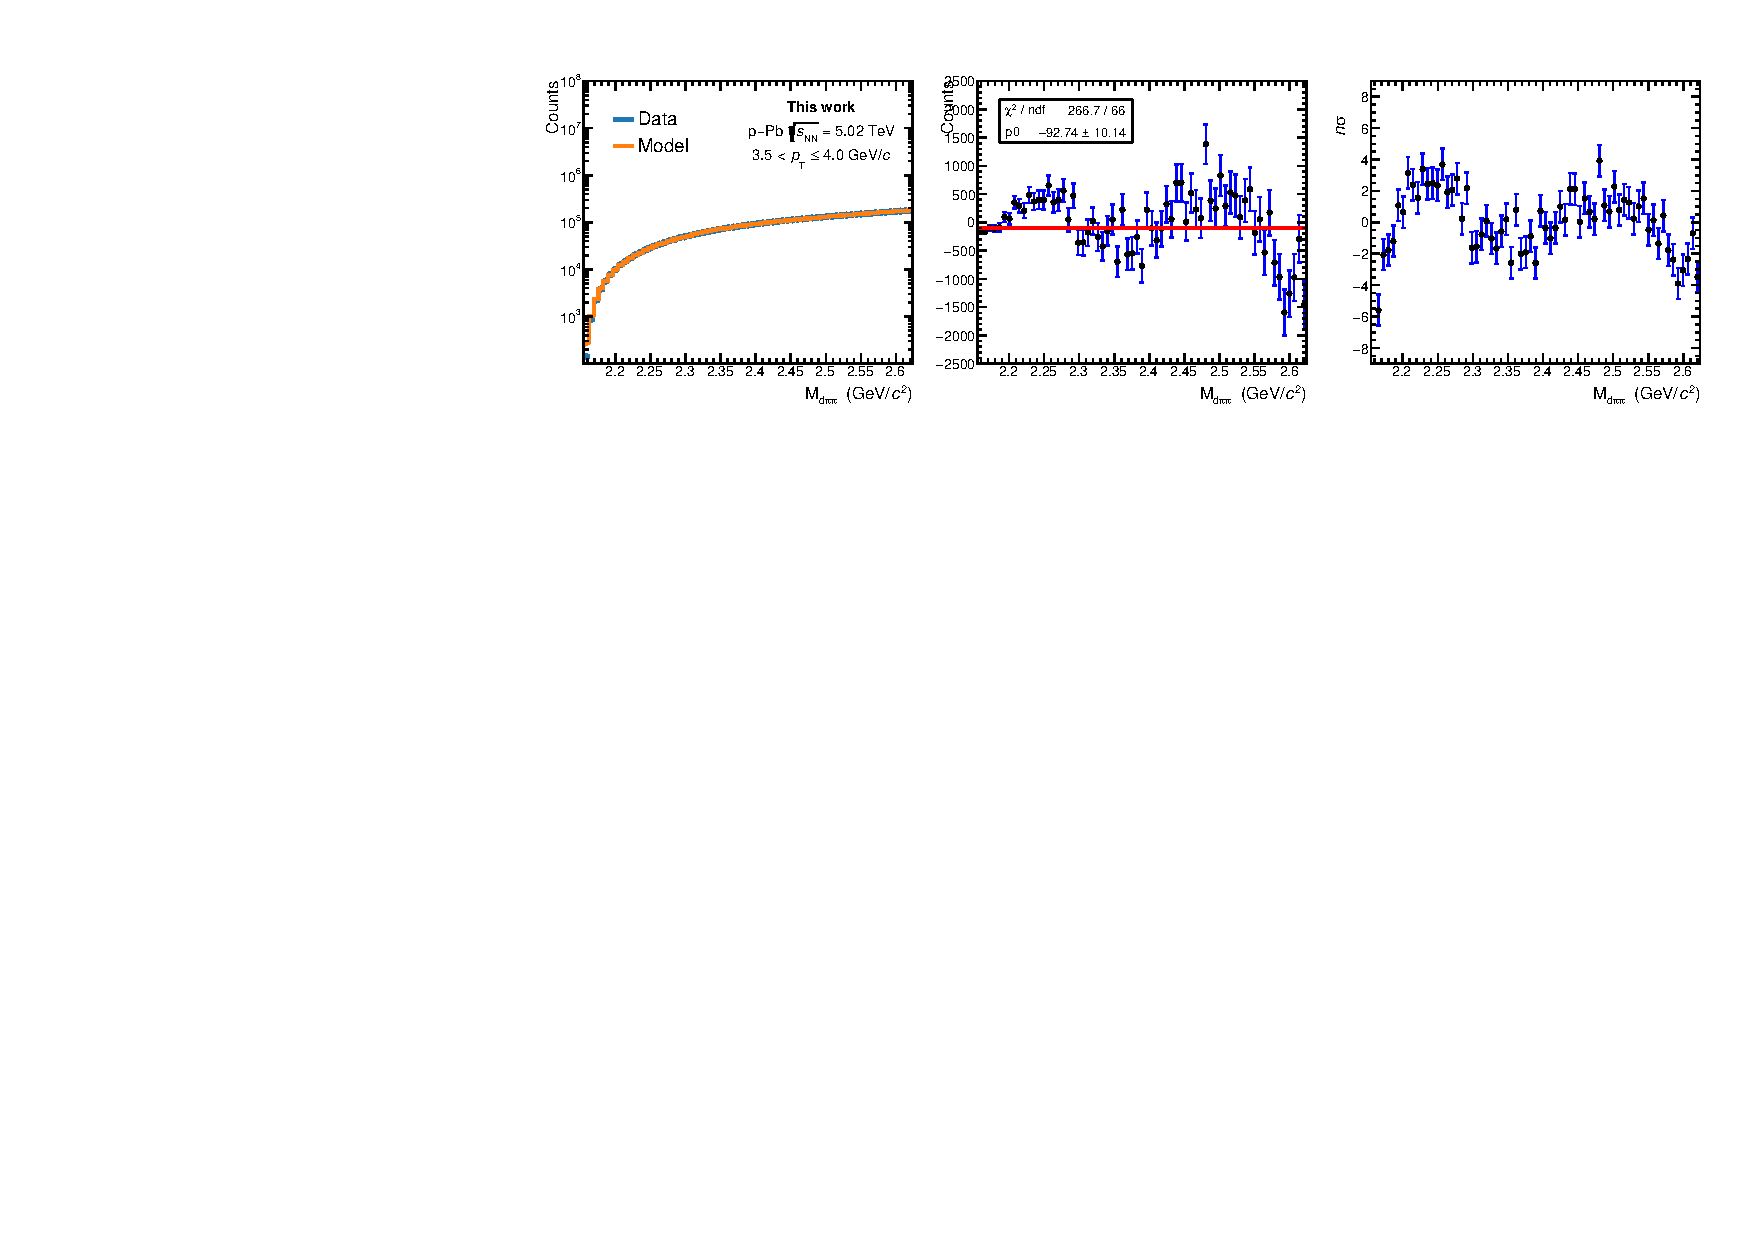
\includegraphics[width=\textwidth]{gfx/appendix/backsub/canvas7}
    \caption{Left panel shows the background model compared with \minv, in the $3.5 < \pt \leq 4.0$ \gevc interval. In the central panel the residual discrepancies are fitted with a constant function, while in the right panel the pull distribution is reported.}
\end{figure}



\end{appendices}